%%%%%%%%%%%%%%%%%%%%%%%%%%%%%%%%%%%%%%%%%
% Journal Article
% LaTeX Template
% Version 1.3 (9/9/13)
%
% This template has been downloaded from:
% http://www.LaTeXTemplates.com
%
% Original author:
% Frits Wenneker (http://www.howtotex.com)
%
% License:
% CC BY-NC-SA 3.0 (http://creativecommons.org/licenses/by-nc-sa/3.0/)
%
%%%%%%%%%%%%%%%%%%%%%%%%%%%%%%%%%%%%%%%%%

%----------------------------------------------------------------------------------------
%	PACKAGES AND OTHER DOCUMENT CONFIGURATIONS
%----------------------------------------------------------------------------------------

\documentclass[twoside]{article}

% consonants
\usepackage[utf8]{inputenc}
\usepackage[T1]{fontenc}

\usepackage{lipsum} % Package to generate dummy text throughout this template

\usepackage[sc]{mathpazo} % Use the Palatino font
\usepackage[T1]{fontenc} % Use 8-bit encoding that has 256 glyphs
\linespread{1.05} % Line spacing - Palatino needs more space between lines
\usepackage{microtype} % Slightly tweak font spacing for aesthetics

\usepackage[hmarginratio=1:1,top=32mm,columnsep=20pt]{geometry} % Document margins
\usepackage{multicol} % Used for the two-column layout of the document
\usepackage[hang, small,labelfont=bf,up,textfont=it,up]{caption} % Custom captions under/above floats in tables or figures
\usepackage{booktabs} % Horizontal rules in tables
\usepackage{float} % Required for tables and figures in the multi-column environment - they need to be placed in specific locations with the [H] (e.g. \begin{table}[H])
\usepackage{hyperref} % For hyperlinks in the PDF
\usepackage{wrapfig}
\usepackage{caption}

\usepackage{lettrine} % The lettrine is the first enlarged letter at the beginning of the text
\usepackage{paralist} % Used for the compactitem environment which makes bullet points with less space between them

\usepackage{verbatimbox} % Used for adding additional vertical space to mathematical tabular sections

\usepackage{adjustbox}
\usepackage{graphicx}

\usepackage{nth}

\usepackage[natbib = true, style=authoryear, url = false, doi=false,isbn=false,  maxbibnames=9,maxcitenames=1,uniquelist=false, backend=biber]{biblatex}
\addbibresource{Remote.bib}
%\addbibresource{Rpackage.bib}

% \usepackage[natbib = true, style=authoryear, url = true]{biblatex} % distribution version that includes url to the paper
% For removing the "in:" after the author
\renewbibmacro{in:}{}
\renewbibmacro{in:}{%
  \ifentrytype{article}{}{\printtext{\bibstring{in}\intitlepunct}}}

\usepackage{abstract} % Allows abstract customization
\renewcommand{\abstractnamefont}{\normalfont\bfseries} % Set the "Abstract" text to bold
\renewcommand{\abstracttextfont}{\normalfont\small\itshape} % Set the abstract itself to small italic text

%%%%%%%%
\newcommand*{\captionsource}[2]{%
  \caption[{#1}]{%
    #1%
    \\\hspace{\linewidth}%
    \textbf{Source:} #2%
  }%
}
 
%%%


% own packages
\usepackage{tikz}
\usepackage{standalone}
 \usepackage{listings}
 \usepackage{nth}  % proper superscripts with \nth{1}, \nth2 , etc
 % Table formatting
    \usepackage{tabularx}
    \usepackage{ltablex}

   \usepackage[
singlelinecheck=false % <-- important
]{caption} 

 % \usepackage{amsfonts}
    \usepackage{amsmath}
    \usepackage{amssymb}

\usepackage{enumitem, color, amssymb}

% footnote without number macro
\makeatletter
\def\blfootnote{\xdef\@thefnmark{}\@footnotetext}
\makeatother


\usepackage{titlesec} % Allows customization of titles
\renewcommand\thesection{\Roman{section}} % Roman numerals for the sections
\renewcommand\thesubsection{\Roman{subsection}} % Roman numerals for subsections
\titleformat{\section}[block]{\large\scshape\centering}{\thesection.}{1em}{} % Change the look of the section titles
\titleformat{\subsection}[block]{\large}{\thesubsection.}{1em}{} % Change the look of the section titles

\usepackage{fancyhdr} % Headers and footers
\pagestyle{fancy} % All pages have headers and footers
\fancyhead{} % Blank out the default header
\fancyfoot{} % Blank out the default footer
\fancyhead[C]{TES9130 - Econometrics $\bullet$ Term paper $\bullet$ } % Custom header text
\fancyfoot[RO,LE]{\thepage} % Custom footer text

%----------------------------------------------------------------------------------------
%	TITLE SECTION
%----------------------------------------------------------------------------------------

\title{\vspace{-15mm}\fontsize{18pt}{12pt}\selectfont\textbf{MARKUPS AND THEIR IMPLICIATONS FOR MACROECONOMIC DYNAMICS}} % Article title

\author{
\large
\textsc{Nicolas Reigl} \\ %\thanks{A thank you or further information}\\[2mm] % Your name
\normalsize Tallinn School of Economics and Business Administration 
\normalsize \\ Tallinn University of Technology
\normalsize \\ Akadeemia tee 3, Tallinn, Estonia \\ % Your institution
\normalsize \href{mailto:nicolas.reigl@gmail.com}{nicolas.reigl@gmail.com} % Your email address
\vspace{-5mm}
}
\date{}

%----------------------------------------------------------------------------------------

\begin{document}

\maketitle % Insert title

\thispagestyle{fancy} % All pages have headers and footers

%----------------------------------------------------------------------------------------
%	ABSTRACT
%----------------------------------------------------------------------------------------

\begin{abstract}

\noindent This paper investigates the behaviour of the Estonian markup over the business cycle. The analysis shows that the gross operating surplus and the profit margin indicator approximately move in pro-cyclical patterns with output. Furthermore, the profit margin indicator as proxy of the markup exhibits non-stationary movements over the sample period 1995Q1 to 2014Q2. The analysis of the results from a structural vector autoregressive model indicate that a positive unemployment gap shock is prominent in accounting for the upward trend in the markup on short horizons. Finally, positive profit margin indicator shocks prompt significant positive responses of the Estonian core inflation rate.     % Dummy abstract text

\end{abstract}

%----------------------------------------------------------------------------------------
%	ARTICLE CONTENTS
%----------------------------------------------------------------------------------------

\begin{multicols}{2} % Two-column layout throughout the main article text

\section{Introduction}

\lettrine[nindent=0em,lines=3]{T}he behaviour of markups\footnotemark over the business cycle and their impact on prices has been in the focus of researchers for a long time. Production costs, competivness and markups reflect cyclical conditions of a country's economy. Entrepreneurs react to changes in the economic activites, prices charged by competitors, unit labour costs and other factors. They are determinants how shocks to the costs are translated into how firm's set prices. Therefore, understanding the dynamics of markups is crucial to the understanding of dynamics of inflation \citep{Macallan2008How}.

Markups can be also interpreted as the difference between the actual and the efficient level of output. One way of measuring the markup is over the production function where the markup is the inverse of the labour share of income. Therefore, a widening markup points to shifts in the distribution of income from labour towards capital \citep{Khan2013Markups}.

However, as \citeauthor{Blanchard2008State} noted: \textit{How markups move, in response to what, and why, is however nearly terra incognita for macro.\dots [W]e are a long way from having either a clear picture or convincing theories, and this is clearly an area where research is urgently needed.} (p. 18). 



% footnote section
\blfootnote{\textbf{Disclaimer: }The views expressed are those of the author and do not necessarily represent the official views of Eesti Pank or the Eurosystem. }
\blfootnote{I would like to thank Dmitry Kulikov, Lenno Uusküla and Jaanika Meriküll and the participants of a research meeting at Eesti Pank  for helpful comments. Any errors are my own. }
\footnotetext{In imperfect competitive markets firm's set prices as a mark-up over their marginal costs}



The economic theory on the cyclical behaviour of markups is rather ambiguous.  No single theory provides a solid prediction on how markups move over the business cycle \citep{Klein2011South}. That is for two main reasons: First, the behaviour of the markup varies with movements in demand relative to supply capacity. I will refer to this as ``excess demand''. Therefore, the behaviour of the markup will depend how quickly wages and other costs adjust relative to the speed of price adjustments for any given excess demand. Consider following intuitive example: If prices adjust quickly but wages are sticky, the markup will increase when a positive demand shocks hits the economy. The firm will supply extra output by employing more labour. As wages are sticky, the labour costs transmit only slowly into higher marginal costs whereas prices adapt quickly; prices rise faster than costs, increasing the markup.

The second reasons is that businesses strive for a ``desired'' markup when they set prices. The ``desired'' markup will depend on what firms think will happen to excess demand. Given a current markup, changes in excess demand will affect future profits over time. Various theories of how firms form their expectations and set their current markup exist \citep{Macallan2008How}. 

\citet{Phelps1970Optimal} assumed that firms lower their current prices to expand their costumer base when they anticipate higher sales in the future; then markups would be pro-cyclical. 

Later theoretical models offered explanations why markups should be counter-cyclical. 

During economic expansions firms are less able to collude as their incentive to reduce prices and increase their market share is higher \citep{Rotemberg1986SupergameTheoretic}. 

Also firms try to deter the entry of other firms to the market during economic booms by lowering the markups \citep{Stiglitz1984Price}

Various authors also argumented that markups should be counter-cyclical due to declined elasticity of the aggregate demand and therefore increasing pricing power during economic downturns \citep{Bils1987Cyclical,Okun1981Prices,Klemperer1987Markets}. 


Corporate finance theory suggests that markups are counter-cyclical because during recession, when firms have a low cash flows and a greater difficulty in raising external funds, tend to raise the markups to meet their financing needs \citep{Klemperer1995Competition,Chevalier1996CapitalMarket}. 

There is large empirical evidence concerning the cyclical behaviour of the markup. However,  the evidence is not robust. Results seem to depend on the estimation techniques (the design of the production function in full structural models and the assumptions used to identify the marginal cost of production). 

For the UK \citet{Haskel1995Price} and \citet{Macallan2008How}  have found that markups move in pro-cyclical patterns whereas for the US  markups moved in counter-cyclical patterns \citep{Bils1987Cyclical,Martins1999Levels,Rotemberg1991Markups}. 

Beyond understanding the cylicality of markups researchers have tried to understand also the link between changes in the markups and inflation. Here again, the literature is not conclusive \citep{Klein2011South}. 

\citet{Neiss2001Markup} found a positive correlation between the markups and inflation across OECD countries. He argues that higher markups raise the monetary authorities' incentive to increase output, leading to higher equilibrium rates of inflation. 

A positive link between markups and inflation was also found in \citet{Chirinko2000Market} and \cite{Bowdler2004Testing}. 

In some New Keynesian models a positive link between markups and inflation was found \citep{Ball2005Monetary,Steinsson2003Optimal}. In those models the change in the desired markup tends to transmit to prices via a cost-push shock. 

When looking on the impact of an inflation shock to markups negative correlation was found \citep{Benabou1992Inflation,Banerjee2005Inflation}. \citet{Benabou1992Inflation} stated that higher inflation leads to more price dispersion, which increases competition in costumers markets that leads to decreasing markups. 


This paper looks at the cyclical behaviour of the markups in Estonia at the aggregate of the private sector and assesses the markups impact on inflation dynamics.  

This paper is organized as follows. Section \ref{Measuring}
reviews briefly the existing metrics of the markup and analysis the cyclicality of the markup. Section \ref{data}  gives an overview of the data used in the econometric model. Section \ref{Econometric framework}  discusses the econometric framework.  Section \ref{Results} presents the empirical results. The final section concludes. 

%------------------------------------------------

\section{Measuring the markup and its cyclical pattern}
\label{Measuring}

The markup is the difference between the price that a business charges and its marginal cost. But measuring the markup is tricky. The markup can not be observed directly. Instead it must be estimated. The markup can thought to be proportional to the inverse of labour income share 

\begin{equation}
 \mu = \frac{P}{MC} = \frac{P \times MPL}{W} = \frac{P \times \frac{Y}{L} \eta _{Y,L}}{W} = \frac{\eta _{Y,L}}{S} 
\end{equation}
where $\mu$ is the markup, $P$ is the price, $MC$ is the marginal cost and $S$ denotes the labour share.  $\eta _{Y,L}$ represents elasticity of output with respect to labour input \citep{Klein2011South}. 



Any estimate will depend on how firms combine inputs (such as capital and labour) to produce output. A simple form, where overhead labour inputs are considered in the model was proposed by \cite{Rotemberg1991Markups}. Assuming the production function takes the Cobb-Douglas form of



\begin{equation}
 Y_{t}=A_{t}^\alpha(L_{t}-\bar{L_{t}})^\alpha  K_{t}^{1-\alpha}
\end{equation}
where $Y_{t}$, $K_{t}$, $L_{t}$,  and $A_{t}$ are output, capital input, labour input and labour-augmenting technology, respectively. $\bar{L_{t}}$ denotes the overhead labour. Then the markup is modified to

\begin{equation}
 \frac{P_{t}}{MC_{t}} = \alpha \frac{1_{t}}{S_{t}}(\frac{L_{t}}{L_{t}-\bar{L_{t}}})
\end{equation}
$P_{t}$ denotes the firms' optimal price which can be expressed as a markup over marginal costs $MC_{t}$. The labour share of income, $S_{t}$ equals $\frac{W_{t}L_{t}}{P_{t}Y_{t}}$ where $W_{t}$ denotes the wages. 

Besides estimating the markup indirectly with a production function other measures of markups are available.

\begin{figure}[H]
\centering
\resizebox{10cm}{!}{% Created by tikzDevice version 0.9 on 2015-12-20 19:34:29
% !TEX encoding = UTF-8 Unicode

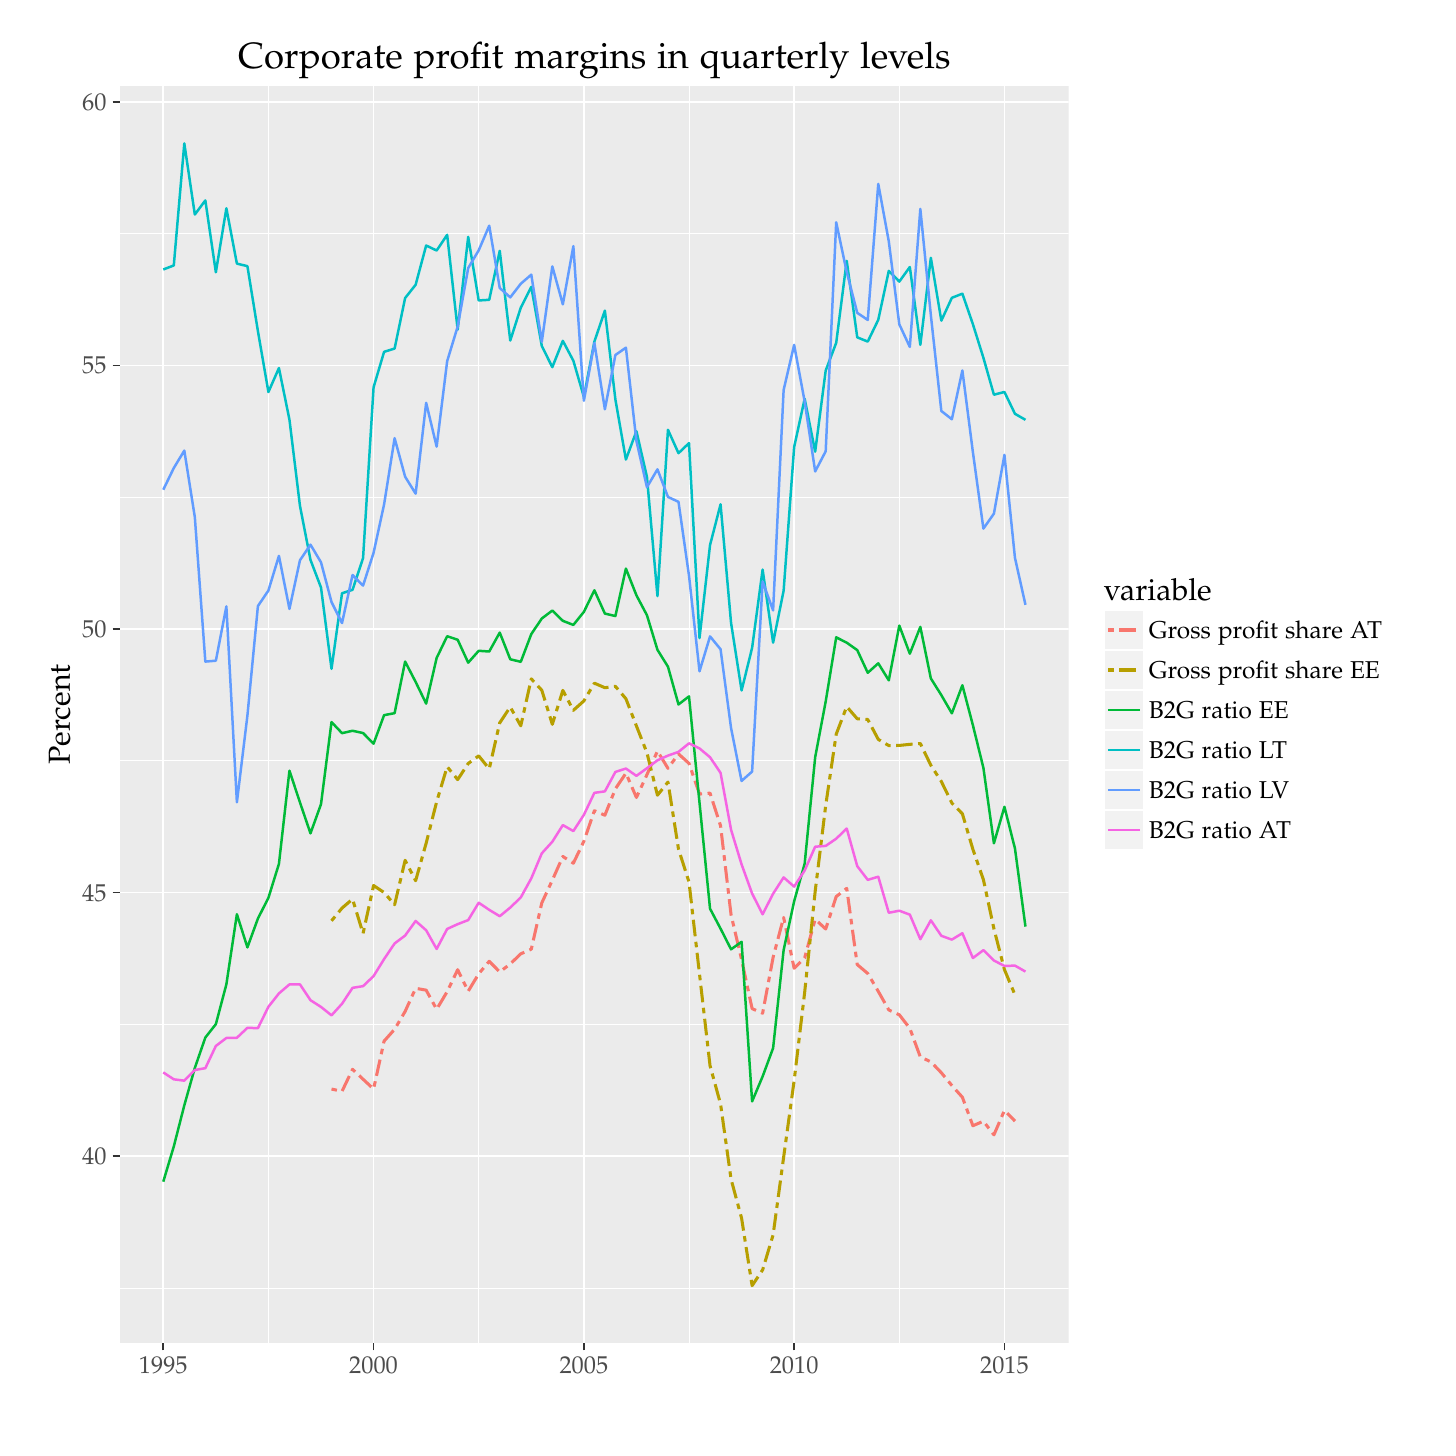
\begin{tikzpicture}[x=1pt,y=1pt]
\definecolor{fillColor}{RGB}{255,255,255}
\path[use as bounding box,fill=fillColor,fill opacity=0.00] (0,0) rectangle (505.89,505.89);
\begin{scope}
\path[clip] (  0.00,  0.00) rectangle (505.89,505.89);
\definecolor{drawColor}{RGB}{255,255,255}
\definecolor{fillColor}{RGB}{255,255,255}

\path[draw=drawColor,line width= 0.6pt,line join=round,line cap=round,fill=fillColor] (  0.00,  0.00) rectangle (505.89,505.89);
\end{scope}
\begin{scope}
\path[clip] ( 33.42, 30.69) rectangle (376.13,484.70);
\definecolor{fillColor}{gray}{0.92}

\path[fill=fillColor] ( 33.42, 30.69) rectangle (376.13,484.70);
\definecolor{drawColor}{RGB}{255,255,255}

\path[draw=drawColor,line width= 0.3pt,line join=round] ( 33.42, 50.46) --
	(376.13, 50.46);

\path[draw=drawColor,line width= 0.3pt,line join=round] ( 33.42,145.71) --
	(376.13,145.71);

\path[draw=drawColor,line width= 0.3pt,line join=round] ( 33.42,240.96) --
	(376.13,240.96);

\path[draw=drawColor,line width= 0.3pt,line join=round] ( 33.42,336.21) --
	(376.13,336.21);

\path[draw=drawColor,line width= 0.3pt,line join=round] ( 33.42,431.46) --
	(376.13,431.46);

\path[draw=drawColor,line width= 0.3pt,line join=round] ( 86.99, 30.69) --
	( 86.99,484.70);

\path[draw=drawColor,line width= 0.3pt,line join=round] (162.98, 30.69) --
	(162.98,484.70);

\path[draw=drawColor,line width= 0.3pt,line join=round] (238.97, 30.69) --
	(238.97,484.70);

\path[draw=drawColor,line width= 0.3pt,line join=round] (314.96, 30.69) --
	(314.96,484.70);

\path[draw=drawColor,line width= 0.6pt,line join=round] ( 33.42, 98.08) --
	(376.13, 98.08);

\path[draw=drawColor,line width= 0.6pt,line join=round] ( 33.42,193.33) --
	(376.13,193.33);

\path[draw=drawColor,line width= 0.6pt,line join=round] ( 33.42,288.58) --
	(376.13,288.58);

\path[draw=drawColor,line width= 0.6pt,line join=round] ( 33.42,383.83) --
	(376.13,383.83);

\path[draw=drawColor,line width= 0.6pt,line join=round] ( 33.42,479.08) --
	(376.13,479.08);

\path[draw=drawColor,line width= 0.6pt,line join=round] ( 49.00, 30.69) --
	( 49.00,484.70);

\path[draw=drawColor,line width= 0.6pt,line join=round] (124.99, 30.69) --
	(124.99,484.70);

\path[draw=drawColor,line width= 0.6pt,line join=round] (200.98, 30.69) --
	(200.98,484.70);

\path[draw=drawColor,line width= 0.6pt,line join=round] (276.96, 30.69) --
	(276.96,484.70);

\path[draw=drawColor,line width= 0.6pt,line join=round] (352.95, 30.69) --
	(352.95,484.70);
\definecolor{drawColor}{RGB}{248,118,109}

\path[draw=drawColor,line width= 1.1pt,dash pattern=on 2pt off 2pt on 6pt off 2pt ,line join=round] (109.79,122.36) --
	(113.59,121.55) --
	(117.39,129.50) --
	(121.19,125.91) --
	(124.99,122.37) --
	(128.79,139.69) --
	(132.59,143.95) --
	(136.39,150.41) --
	(140.19,158.76) --
	(143.99,158.10) --
	(147.78,151.17) --
	(151.58,157.56) --
	(155.38,165.48) --
	(159.18,157.69) --
	(162.98,164.01) --
	(166.78,168.52) --
	(170.58,164.68) --
	(174.38,167.56) --
	(178.18,171.22) --
	(181.98,172.91) --
	(185.78,189.63) --
	(189.58,197.82) --
	(193.38,206.40) --
	(197.18,203.97) --
	(200.98,211.89) --
	(204.78,222.94) --
	(208.57,221.30) --
	(212.37,230.83) --
	(216.17,236.50) --
	(219.97,227.71) --
	(223.77,235.96) --
	(227.57,244.49) --
	(231.37,238.25) --
	(235.17,243.47) --
	(238.97,240.03) --
	(242.77,228.96) --
	(246.57,229.29) --
	(250.37,217.52) --
	(254.17,185.29) --
	(257.97,169.16) --
	(261.77,151.42) --
	(265.57,149.77) --
	(269.36,169.95) --
	(273.16,184.36) --
	(276.96,166.00) --
	(280.76,169.76) --
	(284.56,183.71) --
	(288.36,180.19) --
	(292.16,191.90) --
	(295.96,194.87) --
	(299.76,167.33) --
	(303.56,164.12) --
	(307.36,157.66) --
	(311.16,150.94) --
	(314.96,149.19) --
	(318.76,144.31) --
	(322.56,133.94) --
	(326.36,132.21) --
	(330.15,128.25) --
	(333.95,123.64) --
	(337.75,119.41) --
	(341.55,109.10) --
	(345.35,110.74) --
	(349.15,105.81) --
	(352.95,114.64) --
	(356.75,110.79);
\definecolor{drawColor}{RGB}{183,159,0}

\path[draw=drawColor,line width= 1.1pt,dash pattern=on 2pt off 2pt on 6pt off 2pt ,line join=round] (109.79,183.15) --
	(113.59,187.75) --
	(117.39,191.01) --
	(121.19,178.58) --
	(124.99,195.91) --
	(128.79,193.39) --
	(132.59,188.95) --
	(136.39,205.03) --
	(140.19,197.65) --
	(143.99,211.20) --
	(147.78,226.16) --
	(151.58,238.83) --
	(155.38,234.18) --
	(159.18,239.99) --
	(162.98,242.76) --
	(166.78,238.05) --
	(170.58,254.71) --
	(174.38,260.42) --
	(178.18,253.61) --
	(181.98,270.59) --
	(185.78,266.46) --
	(189.58,254.15) --
	(193.38,266.42) --
	(197.18,259.21) --
	(200.98,262.61) --
	(204.78,269.02) --
	(208.57,267.38) --
	(212.37,267.88) --
	(216.17,263.40) --
	(219.97,253.56) --
	(223.77,243.88) --
	(227.57,228.53) --
	(231.37,233.29) --
	(235.17,209.07) --
	(238.97,197.18) --
	(242.77,163.84) --
	(246.57,130.79) --
	(250.37,116.94) --
	(254.17, 89.78) --
	(257.97, 75.69) --
	(261.77, 51.32) --
	(265.57, 57.00) --
	(269.36, 69.67) --
	(273.16, 97.70) --
	(276.96,125.40) --
	(280.76,157.27) --
	(284.56,193.79) --
	(288.36,224.79) --
	(292.16,250.58) --
	(295.96,260.56) --
	(299.76,256.15) --
	(303.56,255.89) --
	(307.36,248.72) --
	(311.16,246.47) --
	(314.96,246.52) --
	(318.76,246.92) --
	(322.56,247.22) --
	(326.36,239.35) --
	(330.15,233.49) --
	(333.95,225.72) --
	(337.75,221.83) --
	(341.55,208.99) --
	(345.35,198.02) --
	(349.15,180.29) --
	(352.95,165.53) --
	(356.75,156.42);
\definecolor{drawColor}{RGB}{0,186,56}

\path[draw=drawColor,line width= 0.9pt,line join=round] ( 49.00, 88.89) --
	( 52.80,101.62) --
	( 56.60,116.47) --
	( 60.40,129.99) --
	( 64.20,140.97) --
	( 68.00,145.81) --
	( 71.80,160.19) --
	( 75.60,185.53) --
	( 79.40,173.56) --
	( 83.20,183.97) --
	( 86.99,191.46) --
	( 90.79,203.71) --
	( 94.59,237.40) --
	( 98.39,225.93) --
	(102.19,214.75) --
	(105.99,225.29) --
	(109.79,254.97) --
	(113.59,250.96) --
	(117.39,251.82) --
	(121.19,251.00) --
	(124.99,247.17) --
	(128.79,257.47) --
	(132.59,258.18) --
	(136.39,276.83) --
	(140.19,269.47) --
	(143.99,261.64) --
	(147.78,278.14) --
	(151.58,285.99) --
	(155.38,284.71) --
	(159.18,276.43) --
	(162.98,280.72) --
	(166.78,280.46) --
	(170.58,287.30) --
	(174.38,277.66) --
	(178.18,276.74) --
	(181.98,286.75) --
	(185.78,292.40) --
	(189.58,295.26) --
	(193.38,291.55) --
	(197.18,290.07) --
	(200.98,294.79) --
	(204.78,302.59) --
	(208.57,294.17) --
	(212.37,293.28) --
	(216.17,310.42) --
	(219.97,300.77) --
	(223.77,293.59) --
	(227.57,281.07) --
	(231.37,274.98) --
	(235.17,261.33) --
	(238.97,264.25) --
	(242.77,225.77) --
	(246.57,187.53) --
	(250.37,180.32) --
	(254.17,172.85) --
	(257.97,175.56) --
	(261.77,117.90) --
	(265.57,126.91) --
	(269.36,137.17) --
	(273.16,172.56) --
	(276.96,190.22) --
	(280.76,203.77) --
	(284.56,242.26) --
	(288.36,262.38) --
	(292.16,285.58) --
	(295.96,283.66) --
	(299.76,280.97) --
	(303.56,272.78) --
	(307.36,276.20) --
	(311.16,270.06) --
	(314.96,289.83) --
	(318.76,279.68) --
	(322.56,289.35) --
	(326.36,270.74) --
	(330.15,264.70) --
	(333.95,258.13) --
	(337.75,268.27) --
	(341.55,253.85) --
	(345.35,238.42) --
	(349.15,211.16) --
	(352.95,224.35) --
	(356.75,209.31) --
	(360.55,181.06);
\definecolor{drawColor}{RGB}{0,191,196}

\path[draw=drawColor,line width= 0.9pt,line join=round] ( 49.00,418.50) --
	( 52.80,419.97) --
	( 56.60,464.06) --
	( 60.40,438.37) --
	( 64.20,443.46) --
	( 68.00,417.49) --
	( 71.80,440.63) --
	( 75.60,420.62) --
	( 79.40,419.71) --
	( 83.20,396.21) --
	( 86.99,374.23) --
	( 90.79,382.89) --
	( 94.59,364.25) --
	( 98.39,333.10) --
	(102.19,313.58) --
	(105.99,303.59) --
	(109.79,274.22) --
	(113.59,301.51) --
	(117.39,302.75) --
	(121.19,314.21) --
	(124.99,375.94) --
	(128.79,388.76) --
	(132.59,389.93) --
	(136.39,408.19) --
	(140.19,412.99) --
	(143.99,427.17) --
	(147.78,425.36) --
	(151.58,431.02) --
	(155.38,396.74) --
	(159.18,430.29) --
	(162.98,407.31) --
	(166.78,407.55) --
	(170.58,425.25) --
	(174.38,392.82) --
	(178.18,404.69) --
	(181.98,412.22) --
	(185.78,390.85) --
	(189.58,383.21) --
	(193.38,392.72) --
	(197.18,385.54) --
	(200.98,372.46) --
	(204.78,392.46) --
	(208.57,403.65) --
	(212.37,371.53) --
	(216.17,349.83) --
	(219.97,360.07) --
	(223.77,343.58) --
	(227.57,300.50) --
	(231.37,360.57) --
	(235.17,352.13) --
	(238.97,355.76) --
	(242.77,285.33) --
	(246.57,318.93) --
	(250.37,333.66) --
	(254.17,290.76) --
	(257.97,266.38) --
	(261.77,281.77) --
	(265.57,310.08) --
	(269.36,283.67) --
	(273.16,302.42) --
	(276.96,354.32) --
	(280.76,371.78) --
	(284.56,352.67) --
	(288.36,381.97) --
	(292.16,392.00) --
	(295.96,421.63) --
	(299.76,393.99) --
	(303.56,392.45) --
	(307.36,400.32) --
	(311.16,417.99) --
	(314.96,414.14) --
	(318.76,419.39) --
	(322.56,391.28) --
	(326.36,422.74) --
	(330.15,400.02) --
	(333.95,408.26) --
	(337.75,409.77) --
	(341.55,398.75) --
	(345.35,386.59) --
	(349.15,373.26) --
	(352.95,374.25) --
	(356.75,366.36) --
	(360.55,364.18);
\definecolor{drawColor}{RGB}{97,156,255}

\path[draw=drawColor,line width= 0.9pt,line join=round] ( 49.00,338.92) --
	( 52.80,346.76) --
	( 56.60,353.06) --
	( 60.40,329.03) --
	( 64.20,276.82) --
	( 68.00,277.14) --
	( 71.80,296.76) --
	( 75.60,225.97) --
	( 79.40,257.30) --
	( 83.20,296.89) --
	( 86.99,302.50) --
	( 90.79,315.03) --
	( 94.59,295.85) --
	( 98.39,313.43) --
	(102.19,319.06) --
	(105.99,312.71) --
	(109.79,298.34) --
	(113.59,290.75) --
	(117.39,308.10) --
	(121.19,304.28) --
	(124.99,316.13) --
	(128.79,333.62) --
	(132.59,357.54) --
	(136.39,343.63) --
	(140.19,337.50) --
	(143.99,370.33) --
	(147.78,354.50) --
	(151.58,385.37) --
	(155.38,397.89) --
	(159.18,419.02) --
	(162.98,425.43) --
	(166.78,434.33) --
	(170.58,411.82) --
	(174.38,408.43) --
	(178.18,413.35) --
	(181.98,416.64) --
	(185.78,392.38) --
	(189.58,419.62) --
	(193.38,405.91) --
	(197.18,426.93) --
	(200.98,371.07) --
	(204.78,391.95) --
	(208.57,367.99) --
	(212.37,387.60) --
	(216.17,390.25) --
	(219.97,356.54) --
	(223.77,339.84) --
	(227.57,346.29) --
	(231.37,336.31) --
	(235.17,334.55) --
	(238.97,307.85) --
	(242.77,273.32) --
	(246.57,285.92) --
	(250.37,281.28) --
	(254.17,252.78) --
	(257.97,233.69) --
	(261.77,237.08) --
	(265.57,305.74) --
	(269.36,295.31) --
	(273.16,374.95) --
	(276.96,391.26) --
	(280.76,370.81) --
	(284.56,345.54) --
	(288.36,352.81) --
	(292.16,435.56) --
	(295.96,417.60) --
	(299.76,402.84) --
	(303.56,400.27) --
	(307.36,449.42) --
	(311.16,428.67) --
	(314.96,398.69) --
	(318.76,390.52) --
	(322.56,440.39) --
	(326.36,401.98) --
	(330.15,367.37) --
	(333.95,364.39) --
	(337.75,382.02) --
	(341.55,352.52) --
	(345.35,324.87) --
	(349.15,330.29) --
	(352.95,351.51) --
	(356.75,314.32) --
	(360.55,297.33);
\definecolor{drawColor}{RGB}{245,100,227}

\path[draw=drawColor,line width= 0.9pt,line join=round] ( 49.00,128.38) --
	( 52.80,125.87) --
	( 56.60,125.39) --
	( 60.40,129.24) --
	( 64.20,129.90) --
	( 68.00,137.93) --
	( 71.80,140.82) --
	( 75.60,140.89) --
	( 79.40,144.48) --
	( 83.20,144.36) --
	( 86.99,152.08) --
	( 90.79,156.91) --
	( 94.59,160.17) --
	( 98.39,160.17) --
	(102.19,154.47) --
	(105.99,152.03) --
	(109.79,148.99) --
	(113.59,153.18) --
	(117.39,158.93) --
	(121.19,159.54) --
	(124.99,163.17) --
	(128.79,169.32) --
	(132.59,174.96) --
	(136.39,177.83) --
	(140.19,183.09) --
	(143.99,179.73) --
	(147.78,172.98) --
	(151.58,180.21) --
	(155.38,181.94) --
	(159.18,183.41) --
	(162.98,189.68) --
	(166.78,187.12) --
	(170.58,184.81) --
	(174.38,187.94) --
	(178.18,191.59) --
	(181.98,198.49) --
	(185.78,207.54) --
	(189.58,211.73) --
	(193.38,217.74) --
	(197.18,215.58) --
	(200.98,221.44) --
	(204.78,229.40) --
	(208.57,229.92) --
	(212.37,236.95) --
	(216.17,238.17) --
	(219.97,235.54) --
	(223.77,238.28) --
	(227.57,241.15) --
	(231.37,242.85) --
	(235.17,244.19) --
	(238.97,247.29) --
	(242.77,245.44) --
	(246.57,242.26) --
	(250.37,236.61) --
	(254.17,216.04) --
	(257.97,203.54) --
	(261.77,193.02) --
	(265.57,185.52) --
	(269.36,192.94) --
	(273.16,198.84) --
	(276.96,195.51) --
	(280.76,201.34) --
	(284.56,209.93) --
	(288.36,210.22) --
	(292.16,212.82) --
	(295.96,216.50) --
	(299.76,202.91) --
	(303.56,197.95) --
	(307.36,199.09) --
	(311.16,186.06) --
	(314.96,186.80) --
	(318.76,185.38) --
	(322.56,176.49) --
	(326.36,183.34) --
	(330.15,177.73) --
	(333.95,176.36) --
	(337.75,178.67) --
	(341.55,169.70) --
	(345.35,172.55) --
	(349.15,168.81) --
	(352.95,166.84) --
	(356.75,166.96) --
	(360.55,164.80);
\end{scope}
\begin{scope}
\path[clip] (  0.00,  0.00) rectangle (505.89,505.89);
\definecolor{drawColor}{gray}{0.30}

\node[text=drawColor,anchor=base east,inner sep=0pt, outer sep=0pt, scale=  0.88] at ( 28.47, 95.05) {40};

\node[text=drawColor,anchor=base east,inner sep=0pt, outer sep=0pt, scale=  0.88] at ( 28.47,190.30) {45};

\node[text=drawColor,anchor=base east,inner sep=0pt, outer sep=0pt, scale=  0.88] at ( 28.47,285.55) {50};

\node[text=drawColor,anchor=base east,inner sep=0pt, outer sep=0pt, scale=  0.88] at ( 28.47,380.80) {55};

\node[text=drawColor,anchor=base east,inner sep=0pt, outer sep=0pt, scale=  0.88] at ( 28.47,476.05) {60};
\end{scope}
\begin{scope}
\path[clip] (  0.00,  0.00) rectangle (505.89,505.89);
\definecolor{drawColor}{gray}{0.20}

\path[draw=drawColor,line width= 0.6pt,line join=round] ( 30.67, 98.08) --
	( 33.42, 98.08);

\path[draw=drawColor,line width= 0.6pt,line join=round] ( 30.67,193.33) --
	( 33.42,193.33);

\path[draw=drawColor,line width= 0.6pt,line join=round] ( 30.67,288.58) --
	( 33.42,288.58);

\path[draw=drawColor,line width= 0.6pt,line join=round] ( 30.67,383.83) --
	( 33.42,383.83);

\path[draw=drawColor,line width= 0.6pt,line join=round] ( 30.67,479.08) --
	( 33.42,479.08);
\end{scope}
\begin{scope}
\path[clip] (  0.00,  0.00) rectangle (505.89,505.89);
\definecolor{drawColor}{gray}{0.20}

\path[draw=drawColor,line width= 0.6pt,line join=round] ( 49.00, 27.94) --
	( 49.00, 30.69);

\path[draw=drawColor,line width= 0.6pt,line join=round] (124.99, 27.94) --
	(124.99, 30.69);

\path[draw=drawColor,line width= 0.6pt,line join=round] (200.98, 27.94) --
	(200.98, 30.69);

\path[draw=drawColor,line width= 0.6pt,line join=round] (276.96, 27.94) --
	(276.96, 30.69);

\path[draw=drawColor,line width= 0.6pt,line join=round] (352.95, 27.94) --
	(352.95, 30.69);
\end{scope}
\begin{scope}
\path[clip] (  0.00,  0.00) rectangle (505.89,505.89);
\definecolor{drawColor}{gray}{0.30}

\node[text=drawColor,anchor=base,inner sep=0pt, outer sep=0pt, scale=  0.88] at ( 49.00, 19.68) {1995};

\node[text=drawColor,anchor=base,inner sep=0pt, outer sep=0pt, scale=  0.88] at (124.99, 19.68) {2000};

\node[text=drawColor,anchor=base,inner sep=0pt, outer sep=0pt, scale=  0.88] at (200.98, 19.68) {2005};

\node[text=drawColor,anchor=base,inner sep=0pt, outer sep=0pt, scale=  0.88] at (276.96, 19.68) {2010};

\node[text=drawColor,anchor=base,inner sep=0pt, outer sep=0pt, scale=  0.88] at (352.95, 19.68) {2015};
\end{scope}
\begin{scope}
\path[clip] (  0.00,  0.00) rectangle (505.89,505.89);
\definecolor{drawColor}{RGB}{0,0,0}

\node[text=drawColor,anchor=base,inner sep=0pt, outer sep=0pt, scale=  1.10] at (204.78,  7.70) {};
\end{scope}
\begin{scope}
\path[clip] (  0.00,  0.00) rectangle (505.89,505.89);
\definecolor{drawColor}{RGB}{0,0,0}

\node[text=drawColor,rotate= 90.00,anchor=base,inner sep=0pt, outer sep=0pt, scale=  1.10] at ( 15.28,257.69) {Percent};
\end{scope}
\begin{scope}
\path[clip] (  0.00,  0.00) rectangle (505.89,505.89);
\definecolor{fillColor}{RGB}{255,255,255}

\path[fill=fillColor] (384.66,204.47) rectangle (491.85,310.92);
\end{scope}
\begin{scope}
\path[clip] (  0.00,  0.00) rectangle (505.89,505.89);
\definecolor{drawColor}{RGB}{0,0,0}

\node[text=drawColor,anchor=base west,inner sep=0pt, outer sep=0pt, scale=  1.10] at (388.93,299.07) {variable};
\end{scope}
\begin{scope}
\path[clip] (  0.00,  0.00) rectangle (505.89,505.89);
\definecolor{drawColor}{RGB}{255,255,255}
\definecolor{fillColor}{gray}{0.95}

\path[draw=drawColor,line width= 0.6pt,line join=round,line cap=round,fill=fillColor] (388.93,281.01) rectangle (403.38,295.46);
\end{scope}
\begin{scope}
\path[clip] (  0.00,  0.00) rectangle (505.89,505.89);
\definecolor{drawColor}{RGB}{248,118,109}

\path[draw=drawColor,line width= 1.1pt,dash pattern=on 2pt off 2pt on 6pt off 2pt ,line join=round] (390.38,288.23) -- (401.94,288.23);
\end{scope}
\begin{scope}
\path[clip] (  0.00,  0.00) rectangle (505.89,505.89);
\definecolor{drawColor}{RGB}{255,255,255}
\definecolor{fillColor}{gray}{0.95}

\path[draw=drawColor,line width= 0.6pt,line join=round,line cap=round,fill=fillColor] (388.93,266.55) rectangle (403.38,281.01);
\end{scope}
\begin{scope}
\path[clip] (  0.00,  0.00) rectangle (505.89,505.89);
\definecolor{drawColor}{RGB}{183,159,0}

\path[draw=drawColor,line width= 1.1pt,dash pattern=on 2pt off 2pt on 6pt off 2pt ,line join=round] (390.38,273.78) -- (401.94,273.78);
\end{scope}
\begin{scope}
\path[clip] (  0.00,  0.00) rectangle (505.89,505.89);
\definecolor{drawColor}{RGB}{255,255,255}
\definecolor{fillColor}{gray}{0.95}

\path[draw=drawColor,line width= 0.6pt,line join=round,line cap=round,fill=fillColor] (388.93,252.10) rectangle (403.38,266.55);
\end{scope}
\begin{scope}
\path[clip] (  0.00,  0.00) rectangle (505.89,505.89);
\definecolor{drawColor}{RGB}{0,186,56}

\path[draw=drawColor,line width= 0.9pt,line join=round] (390.38,259.33) -- (401.94,259.33);
\end{scope}
\begin{scope}
\path[clip] (  0.00,  0.00) rectangle (505.89,505.89);
\definecolor{drawColor}{RGB}{255,255,255}
\definecolor{fillColor}{gray}{0.95}

\path[draw=drawColor,line width= 0.6pt,line join=round,line cap=round,fill=fillColor] (388.93,237.64) rectangle (403.38,252.10);
\end{scope}
\begin{scope}
\path[clip] (  0.00,  0.00) rectangle (505.89,505.89);
\definecolor{drawColor}{RGB}{0,191,196}

\path[draw=drawColor,line width= 0.9pt,line join=round] (390.38,244.87) -- (401.94,244.87);
\end{scope}
\begin{scope}
\path[clip] (  0.00,  0.00) rectangle (505.89,505.89);
\definecolor{drawColor}{RGB}{255,255,255}
\definecolor{fillColor}{gray}{0.95}

\path[draw=drawColor,line width= 0.6pt,line join=round,line cap=round,fill=fillColor] (388.93,223.19) rectangle (403.38,237.64);
\end{scope}
\begin{scope}
\path[clip] (  0.00,  0.00) rectangle (505.89,505.89);
\definecolor{drawColor}{RGB}{97,156,255}

\path[draw=drawColor,line width= 0.9pt,line join=round] (390.38,230.42) -- (401.94,230.42);
\end{scope}
\begin{scope}
\path[clip] (  0.00,  0.00) rectangle (505.89,505.89);
\definecolor{drawColor}{RGB}{255,255,255}
\definecolor{fillColor}{gray}{0.95}

\path[draw=drawColor,line width= 0.6pt,line join=round,line cap=round,fill=fillColor] (388.93,208.74) rectangle (403.38,223.19);
\end{scope}
\begin{scope}
\path[clip] (  0.00,  0.00) rectangle (505.89,505.89);
\definecolor{drawColor}{RGB}{245,100,227}

\path[draw=drawColor,line width= 0.9pt,line join=round] (390.38,215.96) -- (401.94,215.96);
\end{scope}
\begin{scope}
\path[clip] (  0.00,  0.00) rectangle (505.89,505.89);
\definecolor{drawColor}{RGB}{0,0,0}

\node[text=drawColor,anchor=base west,inner sep=0pt, outer sep=0pt, scale=  0.88] at (405.19,285.20) {Gross profit share AT};
\end{scope}
\begin{scope}
\path[clip] (  0.00,  0.00) rectangle (505.89,505.89);
\definecolor{drawColor}{RGB}{0,0,0}

\node[text=drawColor,anchor=base west,inner sep=0pt, outer sep=0pt, scale=  0.88] at (405.19,270.75) {Gross profit share EE};
\end{scope}
\begin{scope}
\path[clip] (  0.00,  0.00) rectangle (505.89,505.89);
\definecolor{drawColor}{RGB}{0,0,0}

\node[text=drawColor,anchor=base west,inner sep=0pt, outer sep=0pt, scale=  0.88] at (405.19,256.29) {B2G ratio EE};
\end{scope}
\begin{scope}
\path[clip] (  0.00,  0.00) rectangle (505.89,505.89);
\definecolor{drawColor}{RGB}{0,0,0}

\node[text=drawColor,anchor=base west,inner sep=0pt, outer sep=0pt, scale=  0.88] at (405.19,241.84) {B2G ratio LT};
\end{scope}
\begin{scope}
\path[clip] (  0.00,  0.00) rectangle (505.89,505.89);
\definecolor{drawColor}{RGB}{0,0,0}

\node[text=drawColor,anchor=base west,inner sep=0pt, outer sep=0pt, scale=  0.88] at (405.19,227.39) {B2G ratio LV};
\end{scope}
\begin{scope}
\path[clip] (  0.00,  0.00) rectangle (505.89,505.89);
\definecolor{drawColor}{RGB}{0,0,0}

\node[text=drawColor,anchor=base west,inner sep=0pt, outer sep=0pt, scale=  0.88] at (405.19,212.93) {B2G ratio AT};
\end{scope}
\begin{scope}
\path[clip] (  0.00,  0.00) rectangle (505.89,505.89);
\definecolor{drawColor}{RGB}{0,0,0}

\node[text=drawColor,anchor=base,inner sep=0pt, outer sep=0pt, scale=  1.32] at (204.78,491.30) {Corporate profit margins in quarterly levels};
\end{scope}
\end{tikzpicture}

}
\vspace*{-10mm}
\caption{Baltic and Austrian Corporate Profit Margins}\label{fig:Corporate Profit Margins}
\vspace*{-4mm} %get rid of the nas
\caption*{Source: EUROSTAT - namq\_10\_gdp}
\end{figure}


First, the \textit{profit margin} is understood to be the ratio of profits (or ``gross operating surplus'') to gross output . It can be calculated from the national accounts: 


\addvbuffer[12pt 8pt]{
\begin{tabular} { l  }
    Production (P1) \\
      - intermediate consumption (P2) \\
      - compensation of employees (D1) \\
      - net taxes on production (D29-D39)\\
      \hline
      Gross operating surplus (B2G)
\end{tabular}
}


The gross operating surplus margin is defined as the ration of gross operating surplus to value added. Value added (B1G) can be calculated when deducting intermediate consumption (P2) from production (P1). 

Another measurement is the \textit{profit margin indicator}. One way to calculate the profit margin indicator\footnotemark is: 
\begin{equation}
\text{Profit margin indicator} = \frac{\text{YFD}}{\text{NULC}}
\end{equation}

The GDP deflator at basic prices (YFD) is $YFD = YED \times (1-TINYEN)$ where $TINYEN$ is the ratio of indirect taxes net of subsidies to nominal GDP \citep{Kramer2010Methodological}. $NULC$ denotes the nominal unit labour costs. 

\footnotetext{Note that literature sources are not consistent when it comes to the terminology and calculation methodology. The working group on forecasting methodological note has a different term and different calculation method for the profit margin indicator. However, another European Central Bank (ECB) article uses the term ``profit mark-up indicator'' for a similar measurement \citep{Ecb2004Measuring} }


The markup and the profit margin metrics are used in the same context but they are not the same. It can be shown that when the profit margin increases when excess demand increases the markup will increase, in general, too \citep{Macallan2008How}. 

As it is more straightforward to calculate the profit margin indicators, I use the profit margin indicator as proxy of the ``true'' markup. 


In the first step I will analyse the gross operating surplus margin. Figure \ref{fig:Corporate Profit Margins} shows the gross operating surplus margin of Estonia (EE), Latvia (LV) and Lithuania (LT). For comparison I also plot the gross operating margin for Austria (AT).

Also plotted in the figure is the gross profit share for Austria and Estonia. The gross profit share (B2G\_B3G) is equal to the gross operating surplus but also includes mixed income\footnotemark. 

Whereas the gross operating surplus margin has to be calculated manually, the gross profit share can be extracted from EUROSTAT directly. However, as fewer datapoints for the gross profit share are available I use the gross operating surplus margin for the further analysis. 


The markup proxies remain undeflated for the first analysis. It can be seen that the gross operating surplus in levels tends to move in pro-cyclically. For Estonia the profit indicators increased up until 2006. Even before the crises they seem to decrease gradually which might be related to the strong increase in real wages pre-crises. Another reason might be that the Estonian business cycle turned in the \nth{2} quarter of 2007, much before the start of the global financial crises in the \nth{3} quarter of 2008. In late 2009 excess demand seems to pick up again and an increase in the markup proxies is visible for all countries. 

Figure \ref{fig:Corporate Profit Margins} also suggests that the difference between the manually calculated gross operating surplus margin and the gross profit share is more pronounced than expected. 


\begin{figure}[H]
\centering
\resizebox{8cm}{!}{% Created by tikzDevice version 0.9 on 2015-12-20 19:43:08
% !TEX encoding = UTF-8 Unicode
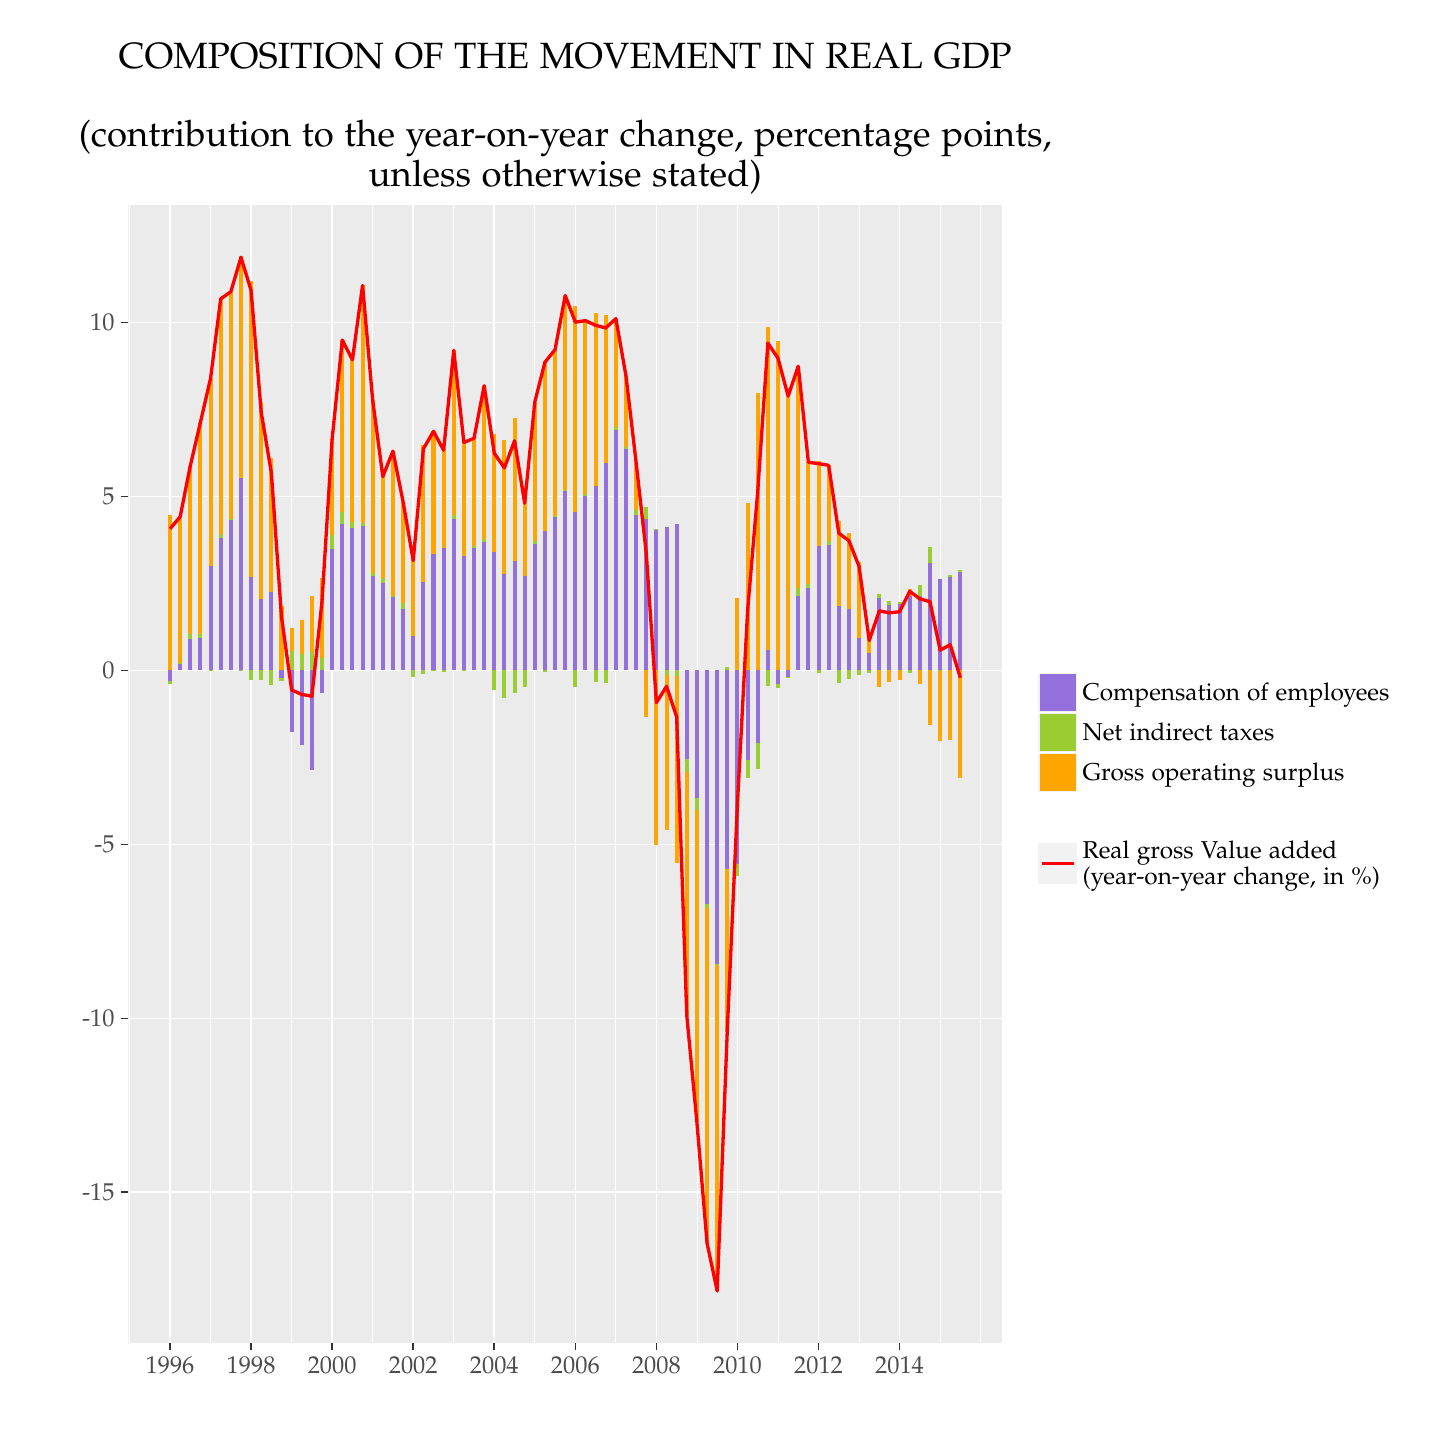
\begin{tikzpicture}[x=1pt,y=1pt]
\definecolor{fillColor}{RGB}{255,255,255}
\path[use as bounding box,fill=fillColor,fill opacity=0.00] (0,0) rectangle (505.89,505.89);
\begin{scope}
\path[clip] (  0.00,  0.00) rectangle (505.89,505.89);
\definecolor{drawColor}{RGB}{255,255,255}
\definecolor{fillColor}{RGB}{255,255,255}

\path[draw=drawColor,line width= 0.6pt,line join=round,line cap=round,fill=fillColor] (  0.00,  0.00) rectangle (505.89,505.89);
\end{scope}
\begin{scope}
\path[clip] ( 36.36, 30.69) rectangle (352.12,441.93);
\definecolor{fillColor}{gray}{0.92}

\path[fill=fillColor] ( 36.36, 30.69) rectangle (352.12,441.93);
\definecolor{drawColor}{RGB}{255,255,255}

\path[draw=drawColor,line width= 0.3pt,line join=round] ( 36.80, 30.69) --
	( 36.80,441.93);

\path[draw=drawColor,line width= 0.3pt,line join=round] ( 66.09, 30.69) --
	( 66.09,441.93);

\path[draw=drawColor,line width= 0.3pt,line join=round] ( 95.38, 30.69) --
	( 95.38,441.93);

\path[draw=drawColor,line width= 0.3pt,line join=round] (124.67, 30.69) --
	(124.67,441.93);

\path[draw=drawColor,line width= 0.3pt,line join=round] (153.96, 30.69) --
	(153.96,441.93);

\path[draw=drawColor,line width= 0.3pt,line join=round] (183.25, 30.69) --
	(183.25,441.93);

\path[draw=drawColor,line width= 0.3pt,line join=round] (212.54, 30.69) --
	(212.54,441.93);

\path[draw=drawColor,line width= 0.3pt,line join=round] (241.83, 30.69) --
	(241.83,441.93);

\path[draw=drawColor,line width= 0.3pt,line join=round] (271.13, 30.69) --
	(271.13,441.93);

\path[draw=drawColor,line width= 0.3pt,line join=round] (300.42, 30.69) --
	(300.42,441.93);

\path[draw=drawColor,line width= 0.3pt,line join=round] (329.71, 30.69) --
	(329.71,441.93);

\path[draw=drawColor,line width= 0.3pt,line join=round] (344.35, 30.69) --
	(344.35,441.93);

\path[draw=drawColor,line width= 0.6pt,line join=round] ( 36.36, 85.05) --
	(352.12, 85.05);

\path[draw=drawColor,line width= 0.6pt,line join=round] ( 36.36,147.91) --
	(352.12,147.91);

\path[draw=drawColor,line width= 0.6pt,line join=round] ( 36.36,210.78) --
	(352.12,210.78);

\path[draw=drawColor,line width= 0.6pt,line join=round] ( 36.36,273.64) --
	(352.12,273.64);

\path[draw=drawColor,line width= 0.6pt,line join=round] ( 36.36,336.51) --
	(352.12,336.51);

\path[draw=drawColor,line width= 0.6pt,line join=round] ( 36.36,399.37) --
	(352.12,399.37);

\path[draw=drawColor,line width= 0.6pt,line join=round] ( 51.44, 30.69) --
	( 51.44,441.93);

\path[draw=drawColor,line width= 0.6pt,line join=round] ( 80.73, 30.69) --
	( 80.73,441.93);

\path[draw=drawColor,line width= 0.6pt,line join=round] (110.02, 30.69) --
	(110.02,441.93);

\path[draw=drawColor,line width= 0.6pt,line join=round] (139.32, 30.69) --
	(139.32,441.93);

\path[draw=drawColor,line width= 0.6pt,line join=round] (168.61, 30.69) --
	(168.61,441.93);

\path[draw=drawColor,line width= 0.6pt,line join=round] (197.90, 30.69) --
	(197.90,441.93);

\path[draw=drawColor,line width= 0.6pt,line join=round] (227.19, 30.69) --
	(227.19,441.93);

\path[draw=drawColor,line width= 0.6pt,line join=round] (256.48, 30.69) --
	(256.48,441.93);

\path[draw=drawColor,line width= 0.6pt,line join=round] (285.77, 30.69) --
	(285.77,441.93);

\path[draw=drawColor,line width= 0.6pt,line join=round] (315.06, 30.69) --
	(315.06,441.93);
\definecolor{fillColor}{RGB}{255,165,0}

\path[fill=fillColor] ( 50.71,273.64) rectangle ( 52.17,329.64);
\definecolor{fillColor}{RGB}{147,112,219}

\path[fill=fillColor] ( 54.37,273.64) rectangle ( 55.84,276.26);
\definecolor{fillColor}{RGB}{154,205,50}

\path[fill=fillColor] ( 54.37,276.26) rectangle ( 55.84,276.40);
\definecolor{fillColor}{RGB}{255,165,0}

\path[fill=fillColor] ( 54.37,276.40) rectangle ( 55.84,329.15);
\definecolor{fillColor}{RGB}{147,112,219}

\path[fill=fillColor] ( 58.03,273.64) rectangle ( 59.50,285.16);
\definecolor{fillColor}{RGB}{154,205,50}

\path[fill=fillColor] ( 58.03,285.16) rectangle ( 59.50,286.71);
\definecolor{fillColor}{RGB}{255,165,0}

\path[fill=fillColor] ( 58.03,286.71) rectangle ( 59.50,347.54);
\definecolor{fillColor}{RGB}{147,112,219}

\path[fill=fillColor] ( 61.69,273.64) rectangle ( 63.16,285.47);
\definecolor{fillColor}{RGB}{154,205,50}

\path[fill=fillColor] ( 61.69,285.47) rectangle ( 63.16,286.68);
\definecolor{fillColor}{RGB}{255,165,0}

\path[fill=fillColor] ( 61.69,286.68) rectangle ( 63.16,363.33);
\definecolor{fillColor}{RGB}{147,112,219}

\path[fill=fillColor] ( 65.35,273.64) rectangle ( 66.82,311.53);
\definecolor{fillColor}{RGB}{255,165,0}

\path[fill=fillColor] ( 65.35,311.53) rectangle ( 66.82,379.45);
\definecolor{fillColor}{RGB}{147,112,219}

\path[fill=fillColor] ( 69.02,273.64) rectangle ( 70.48,321.31);
\definecolor{fillColor}{RGB}{154,205,50}

\path[fill=fillColor] ( 69.02,321.31) rectangle ( 70.48,322.97);
\definecolor{fillColor}{RGB}{255,165,0}

\path[fill=fillColor] ( 69.02,322.97) rectangle ( 70.48,407.91);
\definecolor{fillColor}{RGB}{147,112,219}

\path[fill=fillColor] ( 72.68,273.64) rectangle ( 74.14,328.00);
\definecolor{fillColor}{RGB}{154,205,50}

\path[fill=fillColor] ( 72.68,328.00) rectangle ( 74.14,328.39);
\definecolor{fillColor}{RGB}{255,165,0}

\path[fill=fillColor] ( 72.68,328.39) rectangle ( 74.14,410.46);
\definecolor{fillColor}{RGB}{147,112,219}

\path[fill=fillColor] ( 76.34,273.64) rectangle ( 77.80,343.26);
\definecolor{fillColor}{RGB}{255,165,0}

\path[fill=fillColor] ( 76.34,343.26) rectangle ( 77.80,423.24);
\definecolor{fillColor}{RGB}{147,112,219}

\path[fill=fillColor] ( 80.00,273.64) rectangle ( 81.46,307.23);
\definecolor{fillColor}{RGB}{255,165,0}

\path[fill=fillColor] ( 80.00,307.23) rectangle ( 81.46,414.31);
\definecolor{fillColor}{RGB}{147,112,219}

\path[fill=fillColor] ( 83.66,273.64) rectangle ( 85.13,299.28);
\definecolor{fillColor}{RGB}{255,165,0}

\path[fill=fillColor] ( 83.66,299.28) rectangle ( 85.13,370.54);
\definecolor{fillColor}{RGB}{147,112,219}

\path[fill=fillColor] ( 87.32,273.64) rectangle ( 88.79,301.95);
\definecolor{fillColor}{RGB}{255,165,0}

\path[fill=fillColor] ( 87.32,301.95) rectangle ( 88.79,350.24);

\path[fill=fillColor] ( 90.98,273.64) rectangle ( 92.45,296.89);
\definecolor{fillColor}{RGB}{154,205,50}

\path[fill=fillColor] ( 94.65,273.64) rectangle ( 96.11,280.79);
\definecolor{fillColor}{RGB}{255,165,0}

\path[fill=fillColor] ( 94.65,280.79) rectangle ( 96.11,288.97);
\definecolor{fillColor}{RGB}{154,205,50}

\path[fill=fillColor] ( 98.31,273.64) rectangle ( 99.77,279.50);
\definecolor{fillColor}{RGB}{255,165,0}

\path[fill=fillColor] ( 98.31,279.50) rectangle ( 99.77,291.85);
\definecolor{fillColor}{RGB}{154,205,50}

\path[fill=fillColor] (101.97,273.64) rectangle (103.43,280.44);
\definecolor{fillColor}{RGB}{255,165,0}

\path[fill=fillColor] (101.97,280.44) rectangle (103.43,300.40);
\definecolor{fillColor}{RGB}{154,205,50}

\path[fill=fillColor] (105.63,273.64) rectangle (107.09,278.00);
\definecolor{fillColor}{RGB}{255,165,0}

\path[fill=fillColor] (105.63,278.00) rectangle (107.09,306.95);
\definecolor{fillColor}{RGB}{147,112,219}

\path[fill=fillColor] (109.29,273.64) rectangle (110.76,317.68);
\definecolor{fillColor}{RGB}{154,205,50}

\path[fill=fillColor] (109.29,317.68) rectangle (110.76,322.47);
\definecolor{fillColor}{RGB}{255,165,0}

\path[fill=fillColor] (109.29,322.47) rectangle (110.76,357.37);
\definecolor{fillColor}{RGB}{147,112,219}

\path[fill=fillColor] (112.95,273.64) rectangle (114.42,326.55);
\definecolor{fillColor}{RGB}{154,205,50}

\path[fill=fillColor] (112.95,326.55) rectangle (114.42,330.99);
\definecolor{fillColor}{RGB}{255,165,0}

\path[fill=fillColor] (112.95,330.99) rectangle (114.42,393.01);
\definecolor{fillColor}{RGB}{147,112,219}

\path[fill=fillColor] (116.61,273.64) rectangle (118.08,324.99);
\definecolor{fillColor}{RGB}{154,205,50}

\path[fill=fillColor] (116.61,324.99) rectangle (118.08,327.33);
\definecolor{fillColor}{RGB}{255,165,0}

\path[fill=fillColor] (116.61,327.33) rectangle (118.08,385.84);
\definecolor{fillColor}{RGB}{147,112,219}

\path[fill=fillColor] (120.28,273.64) rectangle (121.74,325.84);
\definecolor{fillColor}{RGB}{154,205,50}

\path[fill=fillColor] (120.28,325.84) rectangle (121.74,326.99);
\definecolor{fillColor}{RGB}{255,165,0}

\path[fill=fillColor] (120.28,326.99) rectangle (121.74,412.72);
\definecolor{fillColor}{RGB}{147,112,219}

\path[fill=fillColor] (123.94,273.64) rectangle (125.40,307.65);
\definecolor{fillColor}{RGB}{154,205,50}

\path[fill=fillColor] (123.94,307.65) rectangle (125.40,308.70);
\definecolor{fillColor}{RGB}{255,165,0}

\path[fill=fillColor] (123.94,308.70) rectangle (125.40,371.24);
\definecolor{fillColor}{RGB}{147,112,219}

\path[fill=fillColor] (127.60,273.64) rectangle (129.06,305.24);
\definecolor{fillColor}{RGB}{154,205,50}

\path[fill=fillColor] (127.60,305.24) rectangle (129.06,306.89);
\definecolor{fillColor}{RGB}{255,165,0}

\path[fill=fillColor] (127.60,306.89) rectangle (129.06,343.66);
\definecolor{fillColor}{RGB}{147,112,219}

\path[fill=fillColor] (131.26,273.64) rectangle (132.72,300.40);
\definecolor{fillColor}{RGB}{154,205,50}

\path[fill=fillColor] (131.26,300.40) rectangle (132.72,300.52);
\definecolor{fillColor}{RGB}{255,165,0}

\path[fill=fillColor] (131.26,300.52) rectangle (132.72,352.87);
\definecolor{fillColor}{RGB}{147,112,219}

\path[fill=fillColor] (134.92,273.64) rectangle (136.39,295.88);
\definecolor{fillColor}{RGB}{154,205,50}

\path[fill=fillColor] (134.92,295.88) rectangle (136.39,298.13);
\definecolor{fillColor}{RGB}{255,165,0}

\path[fill=fillColor] (134.92,298.13) rectangle (136.39,334.55);
\definecolor{fillColor}{RGB}{147,112,219}

\path[fill=fillColor] (138.58,273.64) rectangle (140.05,285.95);
\definecolor{fillColor}{RGB}{255,165,0}

\path[fill=fillColor] (138.58,285.95) rectangle (140.05,315.77);
\definecolor{fillColor}{RGB}{147,112,219}

\path[fill=fillColor] (142.24,273.64) rectangle (143.71,305.69);
\definecolor{fillColor}{RGB}{255,165,0}

\path[fill=fillColor] (142.24,305.69) rectangle (143.71,354.97);
\definecolor{fillColor}{RGB}{147,112,219}

\path[fill=fillColor] (145.91,273.64) rectangle (147.37,315.77);
\definecolor{fillColor}{RGB}{255,165,0}

\path[fill=fillColor] (145.91,315.77) rectangle (147.37,360.31);
\definecolor{fillColor}{RGB}{147,112,219}

\path[fill=fillColor] (149.57,273.64) rectangle (151.03,317.98);
\definecolor{fillColor}{RGB}{255,165,0}

\path[fill=fillColor] (149.57,317.98) rectangle (151.03,353.77);
\definecolor{fillColor}{RGB}{147,112,219}

\path[fill=fillColor] (153.23,273.64) rectangle (154.69,328.22);
\definecolor{fillColor}{RGB}{154,205,50}

\path[fill=fillColor] (153.23,328.22) rectangle (154.69,329.82);
\definecolor{fillColor}{RGB}{255,165,0}

\path[fill=fillColor] (153.23,329.82) rectangle (154.69,389.27);
\definecolor{fillColor}{RGB}{147,112,219}

\path[fill=fillColor] (156.89,273.64) rectangle (158.35,314.87);
\definecolor{fillColor}{RGB}{255,165,0}

\path[fill=fillColor] (156.89,314.87) rectangle (158.35,356.39);
\definecolor{fillColor}{RGB}{147,112,219}

\path[fill=fillColor] (160.55,273.64) rectangle (162.02,318.00);
\definecolor{fillColor}{RGB}{154,205,50}

\path[fill=fillColor] (160.55,318.00) rectangle (162.02,318.72);
\definecolor{fillColor}{RGB}{255,165,0}

\path[fill=fillColor] (160.55,318.72) rectangle (162.02,357.50);
\definecolor{fillColor}{RGB}{147,112,219}

\path[fill=fillColor] (164.21,273.64) rectangle (165.68,319.97);
\definecolor{fillColor}{RGB}{154,205,50}

\path[fill=fillColor] (164.21,319.97) rectangle (165.68,321.01);
\definecolor{fillColor}{RGB}{255,165,0}

\path[fill=fillColor] (164.21,321.01) rectangle (165.68,376.49);
\definecolor{fillColor}{RGB}{147,112,219}

\path[fill=fillColor] (167.87,273.64) rectangle (169.34,316.50);
\definecolor{fillColor}{RGB}{255,165,0}

\path[fill=fillColor] (167.87,316.50) rectangle (169.34,359.23);
\definecolor{fillColor}{RGB}{147,112,219}

\path[fill=fillColor] (171.54,273.64) rectangle (173.00,308.50);
\definecolor{fillColor}{RGB}{255,165,0}

\path[fill=fillColor] (171.54,308.50) rectangle (173.00,356.95);
\definecolor{fillColor}{RGB}{147,112,219}

\path[fill=fillColor] (175.20,273.64) rectangle (176.66,313.30);
\definecolor{fillColor}{RGB}{255,165,0}

\path[fill=fillColor] (175.20,313.30) rectangle (176.66,364.69);
\definecolor{fillColor}{RGB}{147,112,219}

\path[fill=fillColor] (178.86,273.64) rectangle (180.32,307.66);
\definecolor{fillColor}{RGB}{255,165,0}

\path[fill=fillColor] (178.86,307.66) rectangle (180.32,340.10);
\definecolor{fillColor}{RGB}{147,112,219}

\path[fill=fillColor] (182.52,273.64) rectangle (183.98,319.29);
\definecolor{fillColor}{RGB}{154,205,50}

\path[fill=fillColor] (182.52,319.29) rectangle (183.98,320.26);
\definecolor{fillColor}{RGB}{255,165,0}

\path[fill=fillColor] (182.52,320.26) rectangle (183.98,370.67);
\definecolor{fillColor}{RGB}{147,112,219}

\path[fill=fillColor] (186.18,273.64) rectangle (187.65,324.07);
\definecolor{fillColor}{RGB}{255,165,0}

\path[fill=fillColor] (186.18,324.07) rectangle (187.65,385.40);
\definecolor{fillColor}{RGB}{147,112,219}

\path[fill=fillColor] (189.84,273.64) rectangle (191.31,329.15);
\definecolor{fillColor}{RGB}{154,205,50}

\path[fill=fillColor] (189.84,329.15) rectangle (191.31,329.53);
\definecolor{fillColor}{RGB}{255,165,0}

\path[fill=fillColor] (189.84,329.53) rectangle (191.31,389.55);
\definecolor{fillColor}{RGB}{147,112,219}

\path[fill=fillColor] (193.50,273.64) rectangle (194.97,338.58);
\definecolor{fillColor}{RGB}{154,205,50}

\path[fill=fillColor] (193.50,338.58) rectangle (194.97,338.91);
\definecolor{fillColor}{RGB}{255,165,0}

\path[fill=fillColor] (193.50,338.91) rectangle (194.97,409.09);
\definecolor{fillColor}{RGB}{147,112,219}

\path[fill=fillColor] (197.17,273.64) rectangle (198.63,330.78);
\definecolor{fillColor}{RGB}{255,165,0}

\path[fill=fillColor] (197.17,330.78) rectangle (198.63,405.46);
\definecolor{fillColor}{RGB}{147,112,219}

\path[fill=fillColor] (200.83,273.64) rectangle (202.29,336.59);
\definecolor{fillColor}{RGB}{154,205,50}

\path[fill=fillColor] (200.83,336.59) rectangle (202.29,337.22);
\definecolor{fillColor}{RGB}{255,165,0}

\path[fill=fillColor] (200.83,337.22) rectangle (202.29,400.01);
\definecolor{fillColor}{RGB}{147,112,219}

\path[fill=fillColor] (204.49,273.64) rectangle (205.95,340.34);
\definecolor{fillColor}{RGB}{255,165,0}

\path[fill=fillColor] (204.49,340.34) rectangle (205.95,402.62);
\definecolor{fillColor}{RGB}{147,112,219}

\path[fill=fillColor] (208.15,273.64) rectangle (209.61,348.61);
\definecolor{fillColor}{RGB}{255,165,0}

\path[fill=fillColor] (208.15,348.61) rectangle (209.61,401.94);
\definecolor{fillColor}{RGB}{147,112,219}

\path[fill=fillColor] (211.81,273.64) rectangle (213.28,360.39);
\definecolor{fillColor}{RGB}{154,205,50}

\path[fill=fillColor] (211.81,360.39) rectangle (213.28,361.50);
\definecolor{fillColor}{RGB}{255,165,0}

\path[fill=fillColor] (211.81,361.50) rectangle (213.28,400.76);
\definecolor{fillColor}{RGB}{147,112,219}

\path[fill=fillColor] (215.47,273.64) rectangle (216.94,353.57);
\definecolor{fillColor}{RGB}{154,205,50}

\path[fill=fillColor] (215.47,353.57) rectangle (216.94,354.40);
\definecolor{fillColor}{RGB}{255,165,0}

\path[fill=fillColor] (215.47,354.40) rectangle (216.94,380.04);
\definecolor{fillColor}{RGB}{147,112,219}

\path[fill=fillColor] (219.13,273.64) rectangle (220.60,329.90);
\definecolor{fillColor}{RGB}{154,205,50}

\path[fill=fillColor] (219.13,329.90) rectangle (220.60,331.49);
\definecolor{fillColor}{RGB}{255,165,0}

\path[fill=fillColor] (219.13,331.49) rectangle (220.60,348.69);
\definecolor{fillColor}{RGB}{147,112,219}

\path[fill=fillColor] (222.80,273.64) rectangle (224.26,328.21);
\definecolor{fillColor}{RGB}{154,205,50}

\path[fill=fillColor] (222.80,328.21) rectangle (224.26,332.69);
\definecolor{fillColor}{RGB}{147,112,219}

\path[fill=fillColor] (226.46,273.64) rectangle (227.92,324.54);
\definecolor{fillColor}{RGB}{154,205,50}

\path[fill=fillColor] (226.46,324.54) rectangle (227.92,324.91);
\definecolor{fillColor}{RGB}{147,112,219}

\path[fill=fillColor] (230.12,273.64) rectangle (231.58,325.45);

\path[fill=fillColor] (233.78,273.64) rectangle (235.24,326.48);
\definecolor{fillColor}{RGB}{154,205,50}

\path[fill=fillColor] (252.09,273.64) rectangle (253.55,274.80);
\definecolor{fillColor}{RGB}{255,165,0}

\path[fill=fillColor] (255.75,273.64) rectangle (257.21,299.80);

\path[fill=fillColor] (259.41,273.64) rectangle (260.87,334.16);

\path[fill=fillColor] (263.07,273.64) rectangle (264.54,373.73);
\definecolor{fillColor}{RGB}{147,112,219}

\path[fill=fillColor] (266.73,273.64) rectangle (268.20,280.87);
\definecolor{fillColor}{RGB}{255,165,0}

\path[fill=fillColor] (266.73,280.87) rectangle (268.20,397.67);

\path[fill=fillColor] (270.39,273.64) rectangle (271.86,392.78);

\path[fill=fillColor] (274.05,273.64) rectangle (275.52,375.68);
\definecolor{fillColor}{RGB}{147,112,219}

\path[fill=fillColor] (277.72,273.64) rectangle (279.18,300.44);
\definecolor{fillColor}{RGB}{154,205,50}

\path[fill=fillColor] (277.72,300.44) rectangle (279.18,303.49);
\definecolor{fillColor}{RGB}{255,165,0}

\path[fill=fillColor] (277.72,303.49) rectangle (279.18,383.56);
\definecolor{fillColor}{RGB}{147,112,219}

\path[fill=fillColor] (281.38,273.64) rectangle (282.84,303.36);
\definecolor{fillColor}{RGB}{154,205,50}

\path[fill=fillColor] (281.38,303.36) rectangle (282.84,305.00);
\definecolor{fillColor}{RGB}{255,165,0}

\path[fill=fillColor] (281.38,305.00) rectangle (282.84,348.84);
\definecolor{fillColor}{RGB}{147,112,219}

\path[fill=fillColor] (285.04,273.64) rectangle (286.50,318.52);
\definecolor{fillColor}{RGB}{255,165,0}

\path[fill=fillColor] (285.04,318.52) rectangle (286.50,349.20);
\definecolor{fillColor}{RGB}{147,112,219}

\path[fill=fillColor] (288.70,273.64) rectangle (290.17,319.11);
\definecolor{fillColor}{RGB}{154,205,50}

\path[fill=fillColor] (288.70,319.11) rectangle (290.17,320.38);
\definecolor{fillColor}{RGB}{255,165,0}

\path[fill=fillColor] (288.70,320.38) rectangle (290.17,347.74);
\definecolor{fillColor}{RGB}{147,112,219}

\path[fill=fillColor] (292.36,273.64) rectangle (293.83,296.96);
\definecolor{fillColor}{RGB}{255,165,0}

\path[fill=fillColor] (292.36,296.96) rectangle (293.83,327.62);
\definecolor{fillColor}{RGB}{147,112,219}

\path[fill=fillColor] (296.02,273.64) rectangle (297.49,295.68);
\definecolor{fillColor}{RGB}{255,165,0}

\path[fill=fillColor] (296.02,295.68) rectangle (297.49,323.45);
\definecolor{fillColor}{RGB}{147,112,219}

\path[fill=fillColor] (299.68,273.64) rectangle (301.15,285.25);
\definecolor{fillColor}{RGB}{255,165,0}

\path[fill=fillColor] (299.68,285.25) rectangle (301.15,312.73);
\definecolor{fillColor}{RGB}{147,112,219}

\path[fill=fillColor] (303.35,273.64) rectangle (304.81,279.80);
\definecolor{fillColor}{RGB}{255,165,0}

\path[fill=fillColor] (303.35,279.80) rectangle (304.81,285.55);
\definecolor{fillColor}{RGB}{147,112,219}

\path[fill=fillColor] (307.01,273.64) rectangle (308.47,299.74);
\definecolor{fillColor}{RGB}{154,205,50}

\path[fill=fillColor] (307.01,299.74) rectangle (308.47,301.25);
\definecolor{fillColor}{RGB}{147,112,219}

\path[fill=fillColor] (310.67,273.64) rectangle (312.13,297.42);
\definecolor{fillColor}{RGB}{154,205,50}

\path[fill=fillColor] (310.67,297.42) rectangle (312.13,298.60);
\definecolor{fillColor}{RGB}{147,112,219}

\path[fill=fillColor] (314.33,273.64) rectangle (315.79,297.48);
\definecolor{fillColor}{RGB}{154,205,50}

\path[fill=fillColor] (314.33,297.48) rectangle (315.79,298.38);
\definecolor{fillColor}{RGB}{147,112,219}

\path[fill=fillColor] (317.99,273.64) rectangle (319.46,300.41);
\definecolor{fillColor}{RGB}{255,165,0}

\path[fill=fillColor] (317.99,300.41) rectangle (319.46,303.02);
\definecolor{fillColor}{RGB}{147,112,219}

\path[fill=fillColor] (321.65,273.64) rectangle (323.12,300.69);
\definecolor{fillColor}{RGB}{154,205,50}

\path[fill=fillColor] (321.65,300.69) rectangle (323.12,304.60);
\definecolor{fillColor}{RGB}{147,112,219}

\path[fill=fillColor] (325.31,273.64) rectangle (326.78,312.33);
\definecolor{fillColor}{RGB}{154,205,50}

\path[fill=fillColor] (325.31,312.33) rectangle (326.78,318.06);
\definecolor{fillColor}{RGB}{147,112,219}

\path[fill=fillColor] (328.98,273.64) rectangle (330.44,306.63);

\path[fill=fillColor] (332.64,273.64) rectangle (334.10,307.38);
\definecolor{fillColor}{RGB}{154,205,50}

\path[fill=fillColor] (332.64,307.38) rectangle (334.10,308.05);
\definecolor{fillColor}{RGB}{147,112,219}

\path[fill=fillColor] (336.30,273.64) rectangle (337.76,309.30);
\definecolor{fillColor}{RGB}{154,205,50}

\path[fill=fillColor] (336.30,309.30) rectangle (337.76,310.00);
\definecolor{fillColor}{RGB}{147,112,219}

\path[fill=fillColor] ( 50.71,273.64) rectangle ( 52.17,269.74);
\definecolor{fillColor}{RGB}{154,205,50}

\path[fill=fillColor] ( 50.71,269.74) rectangle ( 52.17,268.82);

\path[fill=fillColor] ( 65.35,273.40) rectangle ( 66.82,273.64);

\path[fill=fillColor] ( 76.34,273.31) rectangle ( 77.80,273.64);

\path[fill=fillColor] ( 80.00,270.26) rectangle ( 81.46,273.64);

\path[fill=fillColor] ( 83.66,270.01) rectangle ( 85.13,273.64);

\path[fill=fillColor] ( 87.32,268.42) rectangle ( 88.79,273.64);
\definecolor{fillColor}{RGB}{147,112,219}

\path[fill=fillColor] ( 90.98,273.64) rectangle ( 92.45,270.82);
\definecolor{fillColor}{RGB}{154,205,50}

\path[fill=fillColor] ( 90.98,270.82) rectangle ( 92.45,269.69);
\definecolor{fillColor}{RGB}{147,112,219}

\path[fill=fillColor] ( 94.65,251.23) rectangle ( 96.11,273.64);

\path[fill=fillColor] ( 98.31,246.75) rectangle ( 99.77,273.64);

\path[fill=fillColor] (101.97,237.53) rectangle (103.43,273.64);

\path[fill=fillColor] (105.63,265.29) rectangle (107.09,273.64);
\definecolor{fillColor}{RGB}{154,205,50}

\path[fill=fillColor] (138.58,271.21) rectangle (140.05,273.64);

\path[fill=fillColor] (142.24,272.36) rectangle (143.71,273.64);

\path[fill=fillColor] (145.91,273.35) rectangle (147.37,273.64);

\path[fill=fillColor] (149.57,273.08) rectangle (151.03,273.64);

\path[fill=fillColor] (156.89,273.26) rectangle (158.35,273.64);

\path[fill=fillColor] (167.87,266.48) rectangle (169.34,273.64);

\path[fill=fillColor] (171.54,263.50) rectangle (173.00,273.64);

\path[fill=fillColor] (175.20,265.56) rectangle (176.66,273.64);

\path[fill=fillColor] (178.86,267.58) rectangle (180.32,273.64);

\path[fill=fillColor] (186.18,273.22) rectangle (187.65,273.64);

\path[fill=fillColor] (197.17,267.66) rectangle (198.63,273.64);

\path[fill=fillColor] (204.49,269.34) rectangle (205.95,273.64);

\path[fill=fillColor] (208.15,269.09) rectangle (209.61,273.64);
\definecolor{fillColor}{RGB}{255,165,0}

\path[fill=fillColor] (222.80,256.90) rectangle (224.26,273.64);

\path[fill=fillColor] (226.46,210.72) rectangle (227.92,273.64);
\definecolor{fillColor}{RGB}{154,205,50}

\path[fill=fillColor] (230.12,273.64) rectangle (231.58,272.09);
\definecolor{fillColor}{RGB}{255,165,0}

\path[fill=fillColor] (230.12,272.09) rectangle (231.58,216.08);
\definecolor{fillColor}{RGB}{154,205,50}

\path[fill=fillColor] (233.78,273.64) rectangle (235.24,271.72);
\definecolor{fillColor}{RGB}{255,165,0}

\path[fill=fillColor] (233.78,271.72) rectangle (235.24,204.02);
\definecolor{fillColor}{RGB}{147,112,219}

\path[fill=fillColor] (237.44,273.64) rectangle (238.91,241.46);
\definecolor{fillColor}{RGB}{154,205,50}

\path[fill=fillColor] (237.44,241.46) rectangle (238.91,236.99);
\definecolor{fillColor}{RGB}{255,165,0}

\path[fill=fillColor] (237.44,236.99) rectangle (238.91,148.87);
\definecolor{fillColor}{RGB}{147,112,219}

\path[fill=fillColor] (241.10,273.64) rectangle (242.57,227.35);
\definecolor{fillColor}{RGB}{154,205,50}

\path[fill=fillColor] (241.10,227.35) rectangle (242.57,223.29);
\definecolor{fillColor}{RGB}{255,165,0}

\path[fill=fillColor] (241.10,223.29) rectangle (242.57,110.29);
\definecolor{fillColor}{RGB}{147,112,219}

\path[fill=fillColor] (244.76,273.64) rectangle (246.23,189.09);
\definecolor{fillColor}{RGB}{154,205,50}

\path[fill=fillColor] (244.76,189.09) rectangle (246.23,187.81);
\definecolor{fillColor}{RGB}{255,165,0}

\path[fill=fillColor] (244.76,187.81) rectangle (246.23, 66.62);
\definecolor{fillColor}{RGB}{147,112,219}

\path[fill=fillColor] (248.43,273.64) rectangle (249.89,167.50);
\definecolor{fillColor}{RGB}{154,205,50}

\path[fill=fillColor] (248.43,167.50) rectangle (249.89,167.23);
\definecolor{fillColor}{RGB}{255,165,0}

\path[fill=fillColor] (248.43,167.23) rectangle (249.89, 49.38);
\definecolor{fillColor}{RGB}{147,112,219}

\path[fill=fillColor] (252.09,273.64) rectangle (253.55,201.77);
\definecolor{fillColor}{RGB}{255,165,0}

\path[fill=fillColor] (252.09,201.77) rectangle (253.55,142.87);
\definecolor{fillColor}{RGB}{147,112,219}

\path[fill=fillColor] (255.75,273.64) rectangle (257.21,203.69);
\definecolor{fillColor}{RGB}{154,205,50}

\path[fill=fillColor] (255.75,203.69) rectangle (257.21,199.37);
\definecolor{fillColor}{RGB}{147,112,219}

\path[fill=fillColor] (259.41,273.64) rectangle (260.87,241.22);
\definecolor{fillColor}{RGB}{154,205,50}

\path[fill=fillColor] (259.41,241.22) rectangle (260.87,234.61);
\definecolor{fillColor}{RGB}{147,112,219}

\path[fill=fillColor] (263.07,273.64) rectangle (264.54,247.58);
\definecolor{fillColor}{RGB}{154,205,50}

\path[fill=fillColor] (263.07,247.58) rectangle (264.54,238.15);

\path[fill=fillColor] (266.73,267.89) rectangle (268.20,273.64);
\definecolor{fillColor}{RGB}{147,112,219}

\path[fill=fillColor] (270.39,273.64) rectangle (271.86,268.66);
\definecolor{fillColor}{RGB}{154,205,50}

\path[fill=fillColor] (270.39,268.66) rectangle (271.86,267.26);
\definecolor{fillColor}{RGB}{147,112,219}

\path[fill=fillColor] (274.05,273.64) rectangle (275.52,271.28);
\definecolor{fillColor}{RGB}{154,205,50}

\path[fill=fillColor] (274.05,271.28) rectangle (275.52,270.74);

\path[fill=fillColor] (285.04,272.80) rectangle (286.50,273.64);

\path[fill=fillColor] (292.36,269.23) rectangle (293.83,273.64);

\path[fill=fillColor] (296.02,270.70) rectangle (297.49,273.64);

\path[fill=fillColor] (299.68,272.12) rectangle (301.15,273.64);

\path[fill=fillColor] (303.35,272.54) rectangle (304.81,273.64);
\definecolor{fillColor}{RGB}{255,165,0}

\path[fill=fillColor] (307.01,267.54) rectangle (308.47,273.64);

\path[fill=fillColor] (310.67,269.48) rectangle (312.13,273.64);

\path[fill=fillColor] (314.33,270.10) rectangle (315.79,273.64);
\definecolor{fillColor}{RGB}{154,205,50}

\path[fill=fillColor] (317.99,272.82) rectangle (319.46,273.64);
\definecolor{fillColor}{RGB}{255,165,0}

\path[fill=fillColor] (321.65,268.55) rectangle (323.12,273.64);

\path[fill=fillColor] (325.31,254.03) rectangle (326.78,273.64);
\definecolor{fillColor}{RGB}{154,205,50}

\path[fill=fillColor] (328.98,273.64) rectangle (330.44,273.55);
\definecolor{fillColor}{RGB}{255,165,0}

\path[fill=fillColor] (328.98,273.55) rectangle (330.44,247.98);

\path[fill=fillColor] (332.64,248.50) rectangle (334.10,273.64);

\path[fill=fillColor] (336.30,234.59) rectangle (337.76,273.64);
\definecolor{drawColor}{RGB}{255,0,0}

\path[draw=drawColor,line width= 1.2pt,line join=round] ( 51.44,324.81) --
	( 55.10,329.15) --
	( 58.76,347.54) --
	( 62.43,363.33) --
	( 66.09,379.21) --
	( 69.75,407.91) --
	( 73.41,410.46) --
	( 77.07,422.91) --
	( 80.73,410.92) --
	( 84.39,366.90) --
	( 88.06,345.03) --
	( 91.72,292.94) --
	( 95.38,266.56) --
	( 99.04,264.96) --
	(102.70,264.29) --
	(106.36,298.60) --
	(110.02,357.37) --
	(113.69,393.01) --
	(117.35,385.84) --
	(121.01,412.72) --
	(124.67,371.24) --
	(128.33,343.66) --
	(131.99,352.87) --
	(135.65,334.55) --
	(139.32,313.33) --
	(142.98,353.69) --
	(146.64,360.02) --
	(150.30,353.20) --
	(153.96,389.27) --
	(157.62,356.01) --
	(161.28,357.50) --
	(164.95,376.49) --
	(168.61,352.07) --
	(172.27,346.81) --
	(175.93,356.61) --
	(179.59,334.05) --
	(183.25,370.67) --
	(186.91,384.98) --
	(190.57,389.55) --
	(194.24,409.09) --
	(197.90,399.47) --
	(201.56,400.01) --
	(205.22,398.32) --
	(208.88,397.38) --
	(212.54,400.76) --
	(216.20,380.04) --
	(219.87,348.69) --
	(223.53,315.95) --
	(227.19,261.99) --
	(230.85,267.89) --
	(234.51,256.86) --
	(238.17,148.87) --
	(241.83,110.29) --
	(245.50, 66.62) --
	(249.16, 49.38) --
	(252.82,144.03) --
	(256.48,225.53) --
	(260.14,295.13) --
	(263.80,338.24) --
	(267.46,391.92) --
	(271.13,386.40) --
	(274.79,372.77) --
	(278.45,383.56) --
	(282.11,348.84) --
	(285.77,348.36) --
	(289.43,347.74) --
	(293.09,323.21) --
	(296.76,320.50) --
	(300.42,311.21) --
	(304.08,284.44) --
	(307.74,295.15) --
	(311.40,294.44) --
	(315.06,294.84) --
	(318.72,302.20) --
	(322.39,299.51) --
	(326.05,298.45) --
	(329.71,280.96) --
	(333.37,282.91) --
	(337.03,270.95);
\end{scope}
\begin{scope}
\path[clip] (  0.00,  0.00) rectangle (505.89,505.89);
\definecolor{drawColor}{gray}{0.30}

\node[text=drawColor,anchor=base east,inner sep=0pt, outer sep=0pt, scale=  0.88] at ( 31.41, 82.02) {-15};

\node[text=drawColor,anchor=base east,inner sep=0pt, outer sep=0pt, scale=  0.88] at ( 31.41,144.88) {-10};

\node[text=drawColor,anchor=base east,inner sep=0pt, outer sep=0pt, scale=  0.88] at ( 31.41,207.75) {-5};

\node[text=drawColor,anchor=base east,inner sep=0pt, outer sep=0pt, scale=  0.88] at ( 31.41,270.61) {0};

\node[text=drawColor,anchor=base east,inner sep=0pt, outer sep=0pt, scale=  0.88] at ( 31.41,333.48) {5};

\node[text=drawColor,anchor=base east,inner sep=0pt, outer sep=0pt, scale=  0.88] at ( 31.41,396.34) {10};
\end{scope}
\begin{scope}
\path[clip] (  0.00,  0.00) rectangle (505.89,505.89);
\definecolor{drawColor}{gray}{0.20}

\path[draw=drawColor,line width= 0.6pt,line join=round] ( 33.61, 85.05) --
	( 36.36, 85.05);

\path[draw=drawColor,line width= 0.6pt,line join=round] ( 33.61,147.91) --
	( 36.36,147.91);

\path[draw=drawColor,line width= 0.6pt,line join=round] ( 33.61,210.78) --
	( 36.36,210.78);

\path[draw=drawColor,line width= 0.6pt,line join=round] ( 33.61,273.64) --
	( 36.36,273.64);

\path[draw=drawColor,line width= 0.6pt,line join=round] ( 33.61,336.51) --
	( 36.36,336.51);

\path[draw=drawColor,line width= 0.6pt,line join=round] ( 33.61,399.37) --
	( 36.36,399.37);
\end{scope}
\begin{scope}
\path[clip] (  0.00,  0.00) rectangle (505.89,505.89);
\definecolor{drawColor}{gray}{0.20}

\path[draw=drawColor,line width= 0.6pt,line join=round] ( 51.44, 27.94) --
	( 51.44, 30.69);

\path[draw=drawColor,line width= 0.6pt,line join=round] ( 80.73, 27.94) --
	( 80.73, 30.69);

\path[draw=drawColor,line width= 0.6pt,line join=round] (110.02, 27.94) --
	(110.02, 30.69);

\path[draw=drawColor,line width= 0.6pt,line join=round] (139.32, 27.94) --
	(139.32, 30.69);

\path[draw=drawColor,line width= 0.6pt,line join=round] (168.61, 27.94) --
	(168.61, 30.69);

\path[draw=drawColor,line width= 0.6pt,line join=round] (197.90, 27.94) --
	(197.90, 30.69);

\path[draw=drawColor,line width= 0.6pt,line join=round] (227.19, 27.94) --
	(227.19, 30.69);

\path[draw=drawColor,line width= 0.6pt,line join=round] (256.48, 27.94) --
	(256.48, 30.69);

\path[draw=drawColor,line width= 0.6pt,line join=round] (285.77, 27.94) --
	(285.77, 30.69);

\path[draw=drawColor,line width= 0.6pt,line join=round] (315.06, 27.94) --
	(315.06, 30.69);
\end{scope}
\begin{scope}
\path[clip] (  0.00,  0.00) rectangle (505.89,505.89);
\definecolor{drawColor}{gray}{0.30}

\node[text=drawColor,anchor=base,inner sep=0pt, outer sep=0pt, scale=  0.88] at ( 51.44, 19.68) {1996};

\node[text=drawColor,anchor=base,inner sep=0pt, outer sep=0pt, scale=  0.88] at ( 80.73, 19.68) {1998};

\node[text=drawColor,anchor=base,inner sep=0pt, outer sep=0pt, scale=  0.88] at (110.02, 19.68) {2000};

\node[text=drawColor,anchor=base,inner sep=0pt, outer sep=0pt, scale=  0.88] at (139.32, 19.68) {2002};

\node[text=drawColor,anchor=base,inner sep=0pt, outer sep=0pt, scale=  0.88] at (168.61, 19.68) {2004};

\node[text=drawColor,anchor=base,inner sep=0pt, outer sep=0pt, scale=  0.88] at (197.90, 19.68) {2006};

\node[text=drawColor,anchor=base,inner sep=0pt, outer sep=0pt, scale=  0.88] at (227.19, 19.68) {2008};

\node[text=drawColor,anchor=base,inner sep=0pt, outer sep=0pt, scale=  0.88] at (256.48, 19.68) {2010};

\node[text=drawColor,anchor=base,inner sep=0pt, outer sep=0pt, scale=  0.88] at (285.77, 19.68) {2012};

\node[text=drawColor,anchor=base,inner sep=0pt, outer sep=0pt, scale=  0.88] at (315.06, 19.68) {2014};
\end{scope}
\begin{scope}
\path[clip] (  0.00,  0.00) rectangle (505.89,505.89);
\definecolor{fillColor}{RGB}{255,255,255}

\path[fill=fillColor] (360.65,225.26) rectangle (491.85,280.77);
\end{scope}
\begin{scope}
\path[clip] (  0.00,  0.00) rectangle (505.89,505.89);
\definecolor{drawColor}{RGB}{255,255,255}
\definecolor{fillColor}{gray}{0.95}

\path[draw=drawColor,line width= 0.6pt,line join=round,line cap=round,fill=fillColor] (364.92,258.43) rectangle (379.37,272.89);
\end{scope}
\begin{scope}
\path[clip] (  0.00,  0.00) rectangle (505.89,505.89);
\definecolor{fillColor}{RGB}{147,112,219}

\path[fill=fillColor] (365.63,259.14) rectangle (378.66,272.17);
\end{scope}
\begin{scope}
\path[clip] (  0.00,  0.00) rectangle (505.89,505.89);
\definecolor{fillColor}{RGB}{147,112,219}

\path[fill=fillColor] (365.63,259.14) rectangle (378.66,272.17);
\end{scope}
\begin{scope}
\path[clip] (  0.00,  0.00) rectangle (505.89,505.89);
\definecolor{drawColor}{RGB}{255,255,255}
\definecolor{fillColor}{gray}{0.95}

\path[draw=drawColor,line width= 0.6pt,line join=round,line cap=round,fill=fillColor] (364.92,243.98) rectangle (379.37,258.43);
\end{scope}
\begin{scope}
\path[clip] (  0.00,  0.00) rectangle (505.89,505.89);
\definecolor{fillColor}{RGB}{154,205,50}

\path[fill=fillColor] (365.63,244.69) rectangle (378.66,257.72);
\end{scope}
\begin{scope}
\path[clip] (  0.00,  0.00) rectangle (505.89,505.89);
\definecolor{fillColor}{RGB}{154,205,50}

\path[fill=fillColor] (365.63,244.69) rectangle (378.66,257.72);
\end{scope}
\begin{scope}
\path[clip] (  0.00,  0.00) rectangle (505.89,505.89);
\definecolor{drawColor}{RGB}{255,255,255}
\definecolor{fillColor}{gray}{0.95}

\path[draw=drawColor,line width= 0.6pt,line join=round,line cap=round,fill=fillColor] (364.92,229.52) rectangle (379.37,243.98);
\end{scope}
\begin{scope}
\path[clip] (  0.00,  0.00) rectangle (505.89,505.89);
\definecolor{fillColor}{RGB}{255,165,0}

\path[fill=fillColor] (365.63,230.23) rectangle (378.66,243.27);
\end{scope}
\begin{scope}
\path[clip] (  0.00,  0.00) rectangle (505.89,505.89);
\definecolor{fillColor}{RGB}{255,165,0}

\path[fill=fillColor] (365.63,230.23) rectangle (378.66,243.27);
\end{scope}
\begin{scope}
\path[clip] (  0.00,  0.00) rectangle (505.89,505.89);
\definecolor{drawColor}{RGB}{0,0,0}

\node[text=drawColor,anchor=base west,inner sep=0pt, outer sep=0pt, scale=  0.88] at (381.18,262.63) {Compensation of employees};
\end{scope}
\begin{scope}
\path[clip] (  0.00,  0.00) rectangle (505.89,505.89);
\definecolor{drawColor}{RGB}{0,0,0}

\node[text=drawColor,anchor=base west,inner sep=0pt, outer sep=0pt, scale=  0.88] at (381.18,248.17) {Net indirect taxes};
\end{scope}
\begin{scope}
\path[clip] (  0.00,  0.00) rectangle (505.89,505.89);
\definecolor{drawColor}{RGB}{0,0,0}

\node[text=drawColor,anchor=base west,inner sep=0pt, outer sep=0pt, scale=  0.88] at (381.18,233.72) {Gross operating surplus};
\end{scope}
\begin{scope}
\path[clip] (  0.00,  0.00) rectangle (505.89,505.89);
\definecolor{fillColor}{RGB}{255,255,255}

\path[fill=fillColor] (360.65,191.85) rectangle (491.81,219.56);
\end{scope}
\begin{scope}
\path[clip] (  0.00,  0.00) rectangle (505.89,505.89);
\definecolor{drawColor}{RGB}{255,255,255}
\definecolor{fillColor}{gray}{0.95}

\path[draw=drawColor,line width= 0.6pt,line join=round,line cap=round,fill=fillColor] (364.92,196.12) rectangle (379.37,211.68);
\end{scope}
\begin{scope}
\path[clip] (  0.00,  0.00) rectangle (505.89,505.89);
\definecolor{drawColor}{RGB}{255,0,0}

\path[draw=drawColor,line width= 1.2pt,line join=round] (366.37,203.90) -- (377.93,203.90);
\end{scope}
\begin{scope}
\path[clip] (  0.00,  0.00) rectangle (505.89,505.89);
\definecolor{drawColor}{RGB}{0,0,0}

\node[text=drawColor,anchor=base west,inner sep=0pt, outer sep=0pt, scale=  0.88] at (381.18,205.62) {Real gross Value added };

\node[text=drawColor,anchor=base west,inner sep=0pt, outer sep=0pt, scale=  0.88] at (381.18,196.12) {(year-on-year change, in {\%})};
\end{scope}
\begin{scope}
\path[clip] (  0.00,  0.00) rectangle (505.89,505.89);
\definecolor{drawColor}{RGB}{0,0,0}

\node[text=drawColor,anchor=base,inner sep=0pt, outer sep=0pt, scale=  1.32] at (194.24,491.30) {COMPOSITION OF THE MOVEMENT IN REAL GDP};

\node[text=drawColor,anchor=base,inner sep=0pt, outer sep=0pt, scale=  1.32] at (194.24,477.04) {          };

\node[text=drawColor,anchor=base,inner sep=0pt, outer sep=0pt, scale=  1.32] at (194.24,462.79) {(contribution to the year-on-year change, percentage points,};

\node[text=drawColor,anchor=base,inner sep=0pt, outer sep=0pt, scale=  1.32] at (194.24,448.53) {          unless otherwise stated)};
\end{scope}
\end{tikzpicture}
}
\vspace*{-10mm}
\caption{Margins and Real GDP Growth in Estonia}\label{fig:Margins and Real GDP Growth in Estonia}
\vspace*{-4mm} %get rid of the nas
\caption*{Source: EUROSTAT (namq\_10\_gdp)}
\end{figure}



To complete the analysis, it is worth comparing the movement of the profit share of Estonia with that of foreign counterparts. Clearly Estonia has the lowest profit margin among the Baltic states but larger profitability proxies than a Central European country, namely Austria.

 This seems in line with theoretical arguments. The product markets' competitiveness is dependent, among other factors, on the degree of market concentration. The degree of market concentration is furthermore dependent on the extent of liberalisation of economic policies and the enforcement of competition policy.  \citet{Klein2011South} found that the lack of competition and in particular a high concentration across sectors is associated with high markups in South Africa. In that respect the markup in a well developed country in Central Europe should be smaller than in Estonia. Following this argument one might assume that Estonia has better economic policies, more competitive markets and a more advanced economy than Latvia and Lithuania. 


Figure \ref{fig:Margins and Real GDP Growth in Estonia} shows the change real GDP growth and its composition. The figure shows that, from an income angle, the rise in the gross operating surplus was contributing heavily to GDP growth in pre-crises years. At the same time compensation of employees also rose steadily in the pre-crises years and seems volatile. Starting in the second quarter of 2007 the change in the gross operating surplus experienced an unprecedented decrease. Interestingly, the gross operating surplus margin growth turned negative in 2012 again but the compensation of employees growth increased, which resembles pre-crises dynamics. 


\begin{figure}[H]
% \centering
\resizebox{8cm}{!}{% Created by tikzDevice version 0.9 on 2015-12-31 00:08:52
% !TEX encoding = UTF-8 Unicode
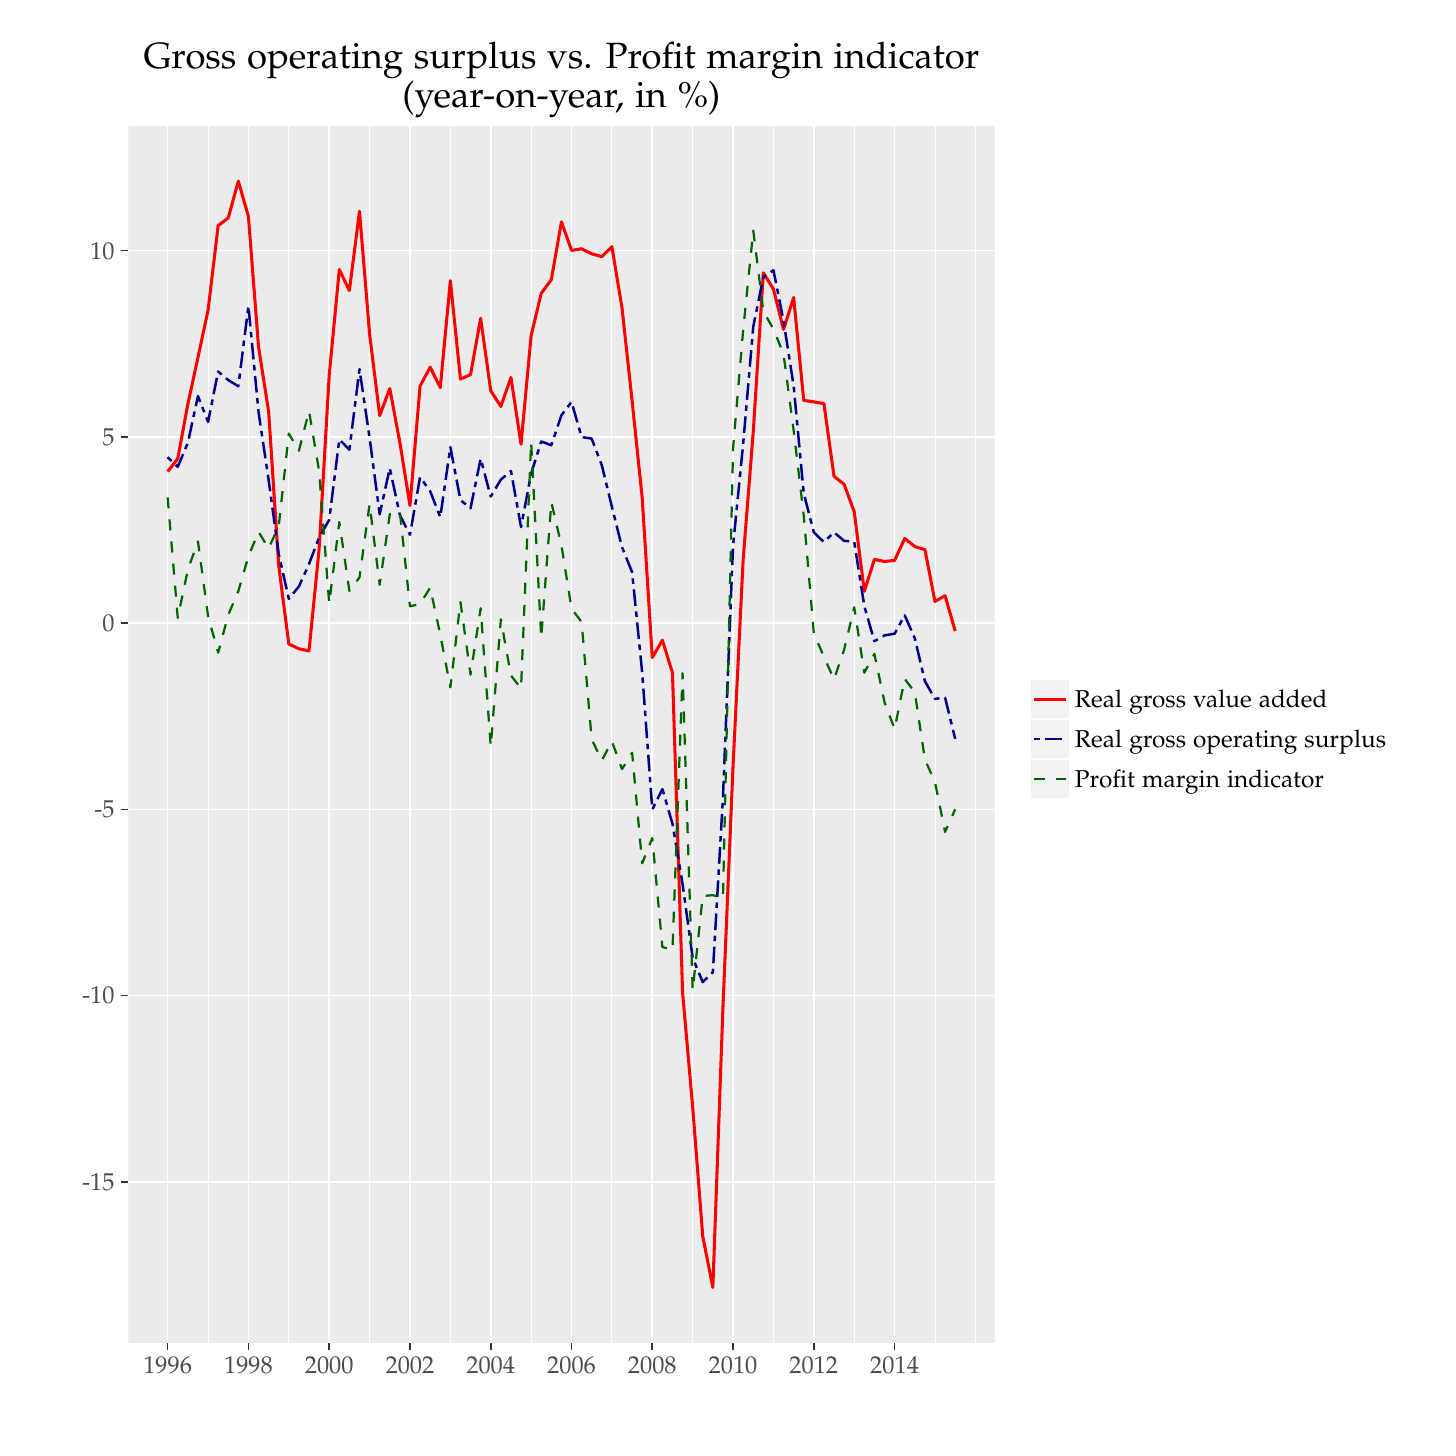
\begin{tikzpicture}[x=1pt,y=1pt]
\definecolor{fillColor}{RGB}{255,255,255}
\path[use as bounding box,fill=fillColor,fill opacity=0.00] (0,0) rectangle (505.89,505.89);
\begin{scope}
\path[clip] (  0.00,  0.00) rectangle (505.89,505.89);
\definecolor{drawColor}{RGB}{255,255,255}
\definecolor{fillColor}{RGB}{255,255,255}

\path[draw=drawColor,line width= 0.6pt,line join=round,line cap=round,fill=fillColor] (  0.00,  0.00) rectangle (505.89,505.89);
\end{scope}
\begin{scope}
\path[clip] ( 36.36, 30.69) rectangle (349.38,470.44);
\definecolor{fillColor}{gray}{0.92}

\path[fill=fillColor] ( 36.36, 30.69) rectangle (349.38,470.44);
\definecolor{drawColor}{RGB}{255,255,255}

\path[draw=drawColor,line width= 0.3pt,line join=round] ( 65.18, 30.69) --
	( 65.18,470.44);

\path[draw=drawColor,line width= 0.3pt,line join=round] ( 94.36, 30.69) --
	( 94.36,470.44);

\path[draw=drawColor,line width= 0.3pt,line join=round] (123.55, 30.69) --
	(123.55,470.44);

\path[draw=drawColor,line width= 0.3pt,line join=round] (152.74, 30.69) --
	(152.74,470.44);

\path[draw=drawColor,line width= 0.3pt,line join=round] (181.92, 30.69) --
	(181.92,470.44);

\path[draw=drawColor,line width= 0.3pt,line join=round] (211.11, 30.69) --
	(211.11,470.44);

\path[draw=drawColor,line width= 0.3pt,line join=round] (240.30, 30.69) --
	(240.30,470.44);

\path[draw=drawColor,line width= 0.3pt,line join=round] (269.48, 30.69) --
	(269.48,470.44);

\path[draw=drawColor,line width= 0.3pt,line join=round] (298.67, 30.69) --
	(298.67,470.44);

\path[draw=drawColor,line width= 0.3pt,line join=round] (327.85, 30.69) --
	(327.85,470.44);

\path[draw=drawColor,line width= 0.3pt,line join=round] (342.45, 30.69) --
	(342.45,470.44);

\path[draw=drawColor,line width= 0.6pt,line join=round] ( 36.36, 88.83) --
	(349.38, 88.83);

\path[draw=drawColor,line width= 0.6pt,line join=round] ( 36.36,156.13) --
	(349.38,156.13);

\path[draw=drawColor,line width= 0.6pt,line join=round] ( 36.36,223.42) --
	(349.38,223.42);

\path[draw=drawColor,line width= 0.6pt,line join=round] ( 36.36,290.72) --
	(349.38,290.72);

\path[draw=drawColor,line width= 0.6pt,line join=round] ( 36.36,358.01) --
	(349.38,358.01);

\path[draw=drawColor,line width= 0.6pt,line join=round] ( 36.36,425.31) --
	(349.38,425.31);

\path[draw=drawColor,line width= 0.6pt,line join=round] ( 50.58, 30.69) --
	( 50.58,470.44);

\path[draw=drawColor,line width= 0.6pt,line join=round] ( 79.77, 30.69) --
	( 79.77,470.44);

\path[draw=drawColor,line width= 0.6pt,line join=round] (108.96, 30.69) --
	(108.96,470.44);

\path[draw=drawColor,line width= 0.6pt,line join=round] (138.14, 30.69) --
	(138.14,470.44);

\path[draw=drawColor,line width= 0.6pt,line join=round] (167.33, 30.69) --
	(167.33,470.44);

\path[draw=drawColor,line width= 0.6pt,line join=round] (196.52, 30.69) --
	(196.52,470.44);

\path[draw=drawColor,line width= 0.6pt,line join=round] (225.70, 30.69) --
	(225.70,470.44);

\path[draw=drawColor,line width= 0.6pt,line join=round] (254.89, 30.69) --
	(254.89,470.44);

\path[draw=drawColor,line width= 0.6pt,line join=round] (284.07, 30.69) --
	(284.07,470.44);

\path[draw=drawColor,line width= 0.6pt,line join=round] (313.26, 30.69) --
	(313.26,470.44);
\definecolor{drawColor}{RGB}{255,0,0}

\path[draw=drawColor,line width= 1.1pt,line join=round] ( 50.58,345.48) --
	( 54.23,350.15) --
	( 57.88,369.83) --
	( 61.53,386.71) --
	( 65.18,403.73) --
	( 68.83,434.37) --
	( 72.47,437.12) --
	( 76.12,450.45) --
	( 79.77,437.63) --
	( 83.42,390.55) --
	( 87.07,367.19) --
	( 90.72,311.44) --
	( 94.36,283.17) --
	( 98.01,281.46) --
	(101.66,280.67) --
	(105.31,317.42) --
	(108.96,380.29) --
	(112.61,418.50) --
	(116.25,410.87) --
	(119.90,439.56) --
	(123.55,395.21) --
	(127.20,365.68) --
	(130.85,375.48) --
	(134.50,355.94) --
	(138.14,333.21) --
	(141.79,376.40) --
	(145.44,383.21) --
	(149.09,375.84) --
	(152.74,414.46) --
	(156.38,378.91) --
	(160.03,380.51) --
	(163.68,400.87) --
	(167.33,374.67) --
	(170.98,369.02) --
	(174.63,379.47) --
	(178.27,355.37) --
	(181.92,394.63) --
	(185.57,409.87) --
	(189.22,414.85) --
	(192.87,435.71) --
	(196.52,425.40) --
	(200.16,425.99) --
	(203.81,424.17) --
	(207.46,423.15) --
	(211.11,426.77) --
	(214.76,404.62) --
	(218.41,371.04) --
	(222.05,336.04) --
	(225.70,278.28) --
	(229.35,284.55) --
	(233.00,272.72) --
	(236.65,157.15) --
	(240.30,115.84) --
	(243.94, 69.11) --
	(247.59, 50.68) --
	(251.24,151.97) --
	(254.89,239.22) --
	(258.54,313.76) --
	(262.19,359.87) --
	(265.83,417.31) --
	(269.48,411.43) --
	(273.13,396.83) --
	(276.78,408.37) --
	(280.43,371.22) --
	(284.07,370.66) --
	(287.72,370.03) --
	(291.37,343.76) --
	(295.02,340.87) --
	(298.67,330.96) --
	(302.32,302.24) --
	(305.96,313.76) --
	(309.61,312.99) --
	(313.26,313.38) --
	(316.91,321.33) --
	(320.56,318.38) --
	(324.21,317.28) --
	(327.85,298.55) --
	(331.50,300.64) --
	(335.15,287.87);
\definecolor{drawColor}{RGB}{0,0,139}

\path[draw=drawColor,line width= 0.9pt,dash pattern=on 2pt off 2pt on 6pt off 2pt ,line join=round] ( 50.58,350.65) --
	( 54.23,347.19) --
	( 57.88,355.84) --
	( 61.53,372.76) --
	( 65.18,363.43) --
	( 68.83,381.62) --
	( 72.47,378.55) --
	( 76.12,376.31) --
	( 79.77,405.33) --
	( 83.42,367.00) --
	( 87.07,342.45) --
	( 90.72,315.64) --
	( 94.36,299.49) --
	( 98.01,303.96) --
	(101.66,312.07) --
	(105.31,321.70) --
	(108.96,328.05) --
	(112.61,357.11) --
	(116.25,353.37) --
	(119.90,382.47) --
	(123.55,357.67) --
	(127.20,330.08) --
	(130.85,346.73) --
	(134.50,329.72) --
	(138.14,322.64) --
	(141.79,343.47) --
	(145.44,338.41) --
	(149.09,329.01) --
	(152.74,354.34) --
	(156.38,335.18) --
	(160.03,332.24) --
	(163.68,350.14) --
	(167.33,336.46) --
	(170.98,342.58) --
	(174.63,345.70) --
	(178.27,325.44) --
	(181.92,344.70) --
	(185.57,356.36) --
	(189.22,354.99) --
	(192.87,365.84) --
	(196.52,370.64) --
	(200.16,357.94) --
	(203.81,357.38) --
	(207.46,347.78) --
	(211.11,332.74) --
	(214.76,318.17) --
	(218.41,309.13) --
	(222.05,272.81) --
	(225.70,223.38) --
	(229.35,230.75) --
	(233.00,218.23) --
	(236.65,196.39) --
	(240.30,169.75) --
	(243.94,160.98) --
	(247.59,164.57) --
	(251.24,227.67) --
	(254.89,318.73) --
	(258.54,355.52) --
	(262.19,397.86) --
	(265.83,415.74) --
	(269.48,418.25) --
	(273.13,399.94) --
	(276.78,376.43) --
	(280.43,337.65) --
	(284.07,323.54) --
	(287.72,320.00) --
	(291.37,323.53) --
	(295.02,320.44) --
	(298.67,320.14) --
	(302.32,296.85) --
	(305.96,284.19) --
	(309.61,286.27) --
	(313.26,286.91) --
	(316.91,293.53) --
	(320.56,285.25) --
	(324.21,269.73) --
	(327.85,263.35) --
	(331.50,263.80) --
	(335.15,248.93);
\definecolor{drawColor}{RGB}{0,100,0}

\path[draw=drawColor,line width= 0.8pt,dash pattern=on 4pt off 4pt ,line join=round] ( 50.58,336.17) --
	( 54.23,292.59) --
	( 57.88,310.04) --
	( 61.53,320.25) --
	( 65.18,293.30) --
	( 68.83,280.03) --
	( 72.47,293.67) --
	( 76.12,302.26) --
	( 79.77,314.91) --
	( 83.42,323.67) --
	( 87.07,317.73) --
	( 90.72,325.80) --
	( 94.36,359.22) --
	( 98.01,352.99) --
	(101.66,367.36) --
	(105.31,345.71) --
	(108.96,297.82) --
	(112.61,327.23) --
	(116.25,302.38) --
	(119.90,307.26) --
	(123.55,333.70) --
	(127.20,304.57) --
	(130.85,330.09) --
	(134.50,330.89) --
	(138.14,296.78) --
	(141.79,297.66) --
	(145.44,303.53) --
	(149.09,286.54) --
	(152.74,267.50) --
	(156.38,298.34) --
	(160.03,272.09) --
	(163.68,296.10) --
	(167.33,246.12) --
	(170.98,292.11) --
	(174.63,271.79) --
	(178.27,267.10) --
	(181.92,356.24) --
	(185.57,285.32) --
	(189.22,334.41) --
	(192.87,318.84) --
	(196.52,295.98) --
	(200.16,291.11) --
	(203.81,248.72) --
	(207.46,241.11) --
	(211.11,247.99) --
	(214.76,237.97) --
	(218.41,243.89) --
	(222.05,203.93) --
	(225.70,213.05) --
	(229.35,173.69) --
	(233.00,172.61) --
	(236.65,272.60) --
	(240.30,158.10) --
	(243.94,192.12) --
	(247.59,192.42) --
	(251.24,191.32) --
	(254.89,353.86) --
	(258.54,396.64) --
	(262.19,432.58) --
	(265.83,403.43) --
	(269.48,396.98) --
	(273.13,387.95) --
	(276.78,360.39) --
	(280.43,329.59) --
	(284.07,287.04) --
	(287.72,278.55) --
	(291.37,270.39) --
	(295.02,281.11) --
	(298.67,296.43) --
	(302.32,272.80) --
	(305.96,279.61) --
	(309.61,262.17) --
	(313.26,252.43) --
	(316.91,270.56) --
	(320.56,265.74) --
	(324.21,241.45) --
	(327.85,233.28) --
	(331.50,215.26) --
	(335.15,223.43);
\end{scope}
\begin{scope}
\path[clip] (  0.00,  0.00) rectangle (505.89,505.89);
\definecolor{drawColor}{gray}{0.30}

\node[text=drawColor,anchor=base east,inner sep=0pt, outer sep=0pt, scale=  0.88] at ( 31.41, 85.80) {-15};

\node[text=drawColor,anchor=base east,inner sep=0pt, outer sep=0pt, scale=  0.88] at ( 31.41,153.10) {-10};

\node[text=drawColor,anchor=base east,inner sep=0pt, outer sep=0pt, scale=  0.88] at ( 31.41,220.39) {-5};

\node[text=drawColor,anchor=base east,inner sep=0pt, outer sep=0pt, scale=  0.88] at ( 31.41,287.69) {0};

\node[text=drawColor,anchor=base east,inner sep=0pt, outer sep=0pt, scale=  0.88] at ( 31.41,354.98) {5};

\node[text=drawColor,anchor=base east,inner sep=0pt, outer sep=0pt, scale=  0.88] at ( 31.41,422.28) {10};
\end{scope}
\begin{scope}
\path[clip] (  0.00,  0.00) rectangle (505.89,505.89);
\definecolor{drawColor}{gray}{0.20}

\path[draw=drawColor,line width= 0.6pt,line join=round] ( 33.61, 88.83) --
	( 36.36, 88.83);

\path[draw=drawColor,line width= 0.6pt,line join=round] ( 33.61,156.13) --
	( 36.36,156.13);

\path[draw=drawColor,line width= 0.6pt,line join=round] ( 33.61,223.42) --
	( 36.36,223.42);

\path[draw=drawColor,line width= 0.6pt,line join=round] ( 33.61,290.72) --
	( 36.36,290.72);

\path[draw=drawColor,line width= 0.6pt,line join=round] ( 33.61,358.01) --
	( 36.36,358.01);

\path[draw=drawColor,line width= 0.6pt,line join=round] ( 33.61,425.31) --
	( 36.36,425.31);
\end{scope}
\begin{scope}
\path[clip] (  0.00,  0.00) rectangle (505.89,505.89);
\definecolor{drawColor}{gray}{0.20}

\path[draw=drawColor,line width= 0.6pt,line join=round] ( 50.58, 27.94) --
	( 50.58, 30.69);

\path[draw=drawColor,line width= 0.6pt,line join=round] ( 79.77, 27.94) --
	( 79.77, 30.69);

\path[draw=drawColor,line width= 0.6pt,line join=round] (108.96, 27.94) --
	(108.96, 30.69);

\path[draw=drawColor,line width= 0.6pt,line join=round] (138.14, 27.94) --
	(138.14, 30.69);

\path[draw=drawColor,line width= 0.6pt,line join=round] (167.33, 27.94) --
	(167.33, 30.69);

\path[draw=drawColor,line width= 0.6pt,line join=round] (196.52, 27.94) --
	(196.52, 30.69);

\path[draw=drawColor,line width= 0.6pt,line join=round] (225.70, 27.94) --
	(225.70, 30.69);

\path[draw=drawColor,line width= 0.6pt,line join=round] (254.89, 27.94) --
	(254.89, 30.69);

\path[draw=drawColor,line width= 0.6pt,line join=round] (284.07, 27.94) --
	(284.07, 30.69);

\path[draw=drawColor,line width= 0.6pt,line join=round] (313.26, 27.94) --
	(313.26, 30.69);
\end{scope}
\begin{scope}
\path[clip] (  0.00,  0.00) rectangle (505.89,505.89);
\definecolor{drawColor}{gray}{0.30}

\node[text=drawColor,anchor=base,inner sep=0pt, outer sep=0pt, scale=  0.88] at ( 50.58, 19.68) {1996};

\node[text=drawColor,anchor=base,inner sep=0pt, outer sep=0pt, scale=  0.88] at ( 79.77, 19.68) {1998};

\node[text=drawColor,anchor=base,inner sep=0pt, outer sep=0pt, scale=  0.88] at (108.96, 19.68) {2000};

\node[text=drawColor,anchor=base,inner sep=0pt, outer sep=0pt, scale=  0.88] at (138.14, 19.68) {2002};

\node[text=drawColor,anchor=base,inner sep=0pt, outer sep=0pt, scale=  0.88] at (167.33, 19.68) {2004};

\node[text=drawColor,anchor=base,inner sep=0pt, outer sep=0pt, scale=  0.88] at (196.52, 19.68) {2006};

\node[text=drawColor,anchor=base,inner sep=0pt, outer sep=0pt, scale=  0.88] at (225.70, 19.68) {2008};

\node[text=drawColor,anchor=base,inner sep=0pt, outer sep=0pt, scale=  0.88] at (254.89, 19.68) {2010};

\node[text=drawColor,anchor=base,inner sep=0pt, outer sep=0pt, scale=  0.88] at (284.07, 19.68) {2012};

\node[text=drawColor,anchor=base,inner sep=0pt, outer sep=0pt, scale=  0.88] at (313.26, 19.68) {2014};
\end{scope}
\begin{scope}
\path[clip] (  0.00,  0.00) rectangle (505.89,505.89);
\definecolor{fillColor}{RGB}{255,255,255}

\path[fill=fillColor] (357.91,222.81) rectangle (491.85,278.32);
\end{scope}
\begin{scope}
\path[clip] (  0.00,  0.00) rectangle (505.89,505.89);
\definecolor{drawColor}{RGB}{255,255,255}
\definecolor{fillColor}{gray}{0.95}

\path[draw=drawColor,line width= 0.6pt,line join=round,line cap=round,fill=fillColor] (362.18,255.99) rectangle (376.64,270.44);
\end{scope}
\begin{scope}
\path[clip] (  0.00,  0.00) rectangle (505.89,505.89);
\definecolor{drawColor}{RGB}{255,0,0}

\path[draw=drawColor,line width= 1.1pt,line join=round] (363.63,263.21) -- (375.19,263.21);
\end{scope}
\begin{scope}
\path[clip] (  0.00,  0.00) rectangle (505.89,505.89);
\definecolor{drawColor}{RGB}{255,255,255}
\definecolor{fillColor}{gray}{0.95}

\path[draw=drawColor,line width= 0.6pt,line join=round,line cap=round,fill=fillColor] (362.18,241.53) rectangle (376.64,255.99);
\end{scope}
\begin{scope}
\path[clip] (  0.00,  0.00) rectangle (505.89,505.89);
\definecolor{drawColor}{RGB}{0,0,139}

\path[draw=drawColor,line width= 0.9pt,dash pattern=on 2pt off 2pt on 6pt off 2pt ,line join=round] (363.63,248.76) -- (375.19,248.76);
\end{scope}
\begin{scope}
\path[clip] (  0.00,  0.00) rectangle (505.89,505.89);
\definecolor{drawColor}{RGB}{255,255,255}
\definecolor{fillColor}{gray}{0.95}

\path[draw=drawColor,line width= 0.6pt,line join=round,line cap=round,fill=fillColor] (362.18,227.08) rectangle (376.64,241.53);
\end{scope}
\begin{scope}
\path[clip] (  0.00,  0.00) rectangle (505.89,505.89);
\definecolor{drawColor}{RGB}{0,100,0}

\path[draw=drawColor,line width= 0.8pt,dash pattern=on 4pt off 4pt ,line join=round] (363.63,234.30) -- (375.19,234.30);
\end{scope}
\begin{scope}
\path[clip] (  0.00,  0.00) rectangle (505.89,505.89);
\definecolor{drawColor}{RGB}{0,0,0}

\node[text=drawColor,anchor=base west,inner sep=0pt, outer sep=0pt, scale=  0.88] at (378.44,260.18) {Real gross value added};
\end{scope}
\begin{scope}
\path[clip] (  0.00,  0.00) rectangle (505.89,505.89);
\definecolor{drawColor}{RGB}{0,0,0}

\node[text=drawColor,anchor=base west,inner sep=0pt, outer sep=0pt, scale=  0.88] at (378.44,245.73) {Real gross operating surplus};
\end{scope}
\begin{scope}
\path[clip] (  0.00,  0.00) rectangle (505.89,505.89);
\definecolor{drawColor}{RGB}{0,0,0}

\node[text=drawColor,anchor=base west,inner sep=0pt, outer sep=0pt, scale=  0.88] at (378.44,231.27) {Profit margin indicator};
\end{scope}
\begin{scope}
\path[clip] (  0.00,  0.00) rectangle (505.89,505.89);
\definecolor{drawColor}{RGB}{0,0,0}

\node[text=drawColor,anchor=base,inner sep=0pt, outer sep=0pt, scale=  1.32] at (192.87,491.30) {Gross operating surplus vs. Profit margin indicator };

\node[text=drawColor,anchor=base,inner sep=0pt, outer sep=0pt, scale=  1.32] at (192.87,477.04) { (year-on-year, in {\%})};
\end{scope}
\end{tikzpicture}
}
\vspace*{-10mm}
\caption{Gross Operating Surplus vs. Profit Margin Indicator}\label{fig:Gross Operating Surplus vs. Profit Margin Indicator}
\vspace*{-4mm} %get rid of the nas
\caption*{Source: EUROSTAT  (namq\_10\_gdp, namq\_10\_lp\_ulc)}
\end{figure}


It can be seen from Figure \ref{fig:Gross Operating Surplus vs. Profit Margin Indicator} that real GDP and the gross operating surplus exhibit a strong co-movement behaviour. The profit margin indicators' behaviour can be split in pre-crises and post-crises patterns. Pre-crises profit margin indicator shows an erratic rather counter-cyclical behaviour whereas during and in the aftermath of the financial crises it shows a strong positive correlation with the real gross value added. % With respect to the structural vectorautoregressive analysis the strong co-movements of the gross operating surplus might pose an identification problem. 

\blfootnote{A comparison with other middle income countries such as Spain would be desirable. Unfortunately not all inputs for calculating the gross operating surplus are available. }

\footnotetext{Mixed income is the remuneration for the work carried out by the owner (or members of his family) of an unincorporated enterprise. This is referred to as ``mixed income'' as it cannot be distinguished from the entrepreneurial profit of the owner \citep[p 177]{franccois2007understanding}.}

%------------------------------------------------
\section{Data}
\label{data}
The empirical literature is very limited for structural vector autoregressive (SVAR) models that incorporate measures of the markup. \citet{Kim2010Identifying} uses a five-variable model to estimate the effects of a permanent markup shock. The model includes the markup ratio 
($\Delta log (P_{t}/MC_{t})$), the growth of the real wage ($\Delta log (W_{t}/P_{t})$), the growth of per capita output ($\Delta log Y_{t}$), inflation ($\Delta log P_{t}$) and the federal funds rate ($FFR_{t}$).  In the second available paper by \citet{Khan2013Markups} a six variable SVAR includes the oil price growth ($\Delta p_{t}^o$), the mark up ratio growth ($\Delta log (P_{t}/MC_{t})$), the growth of real wages ($\Delta log (W_{t}/P_{t})$), the growth of real capita output ($\Delta log Y_{t}$), the log of the product of the overhead labor factor  ($ log U_{t}$), the inflation ($\Delta logP_{t}$) and the bank rate ($r$). 

Given the novelty of this research for Estonia I rely on a simpler SVAR model with proven identifying restrictions in which I include the profit margin indicator. A five-variable VAR model is constructed to estimate the shocks to the nominal exchange rate (denoted as ``\textit{neer}''), the short-term interest rate (denoted as ``\textit{eemmrate}''), the profit margin indicator (denoted as ``\textit{profitmrg}'') and the core inflation rate (denoted as ``\textit{core}''). The unemplyoment gap (denoted as ``\textit{eeugap}'') is defined as the  difference between the nonaccelerating inflation rate of unemployment (NAIRU) and the unemployment rate. For the NAIRU I use the long-term unemployment  data for Estonia. 

For the nominal exchange rate (NEER) I use the trade-weighted currency index of the EU28 countries. For the short-term interest rate I use the 3-month averages for the euro area countries (EURIBOR) and for the period before Estonia entered the Euro Area system the 3-month rates for Estonia.  The profit margin indicator enters the model as proxy for the markup. The core inflation is defined as Estonias harmonized consumer price index excluding energy, food, alcohol  and tobacco. 

Except for the core inflation rate all data was extracted from Eurostat in quarterly levels. The core inflation rate was downloaded in monthly frequency and later aggregated to quarterly values. The data was seasonally and outlier adjusted. Unfortunately the Eurostat database does not contain complete data for calculating the unemployment gap and the core inflation rate for periods earlier then 1997. Those numbers were obtained from Eesti Pank. In total, the matrix contains 80 observations,  starting in the first quarter of 1995 and ending in the fourth quarter of 2014.  

Figure \ref{fig:time series plots} shows the unemployment gap (\textit{eeugap}) in levels, the log levels of the nominal exchange rate (\textit{lneer}), the short term interest rate in levels (\textit{eemmrate}) and the core inflation in log levels (\textit{lcore}). Whereas the nominal exchange rate and the core inflation series seem to contain a constant, the unemployment gap series and the profit margin indicator resemble non-stationary processes without a constant or trend. For the short-term interest rate a structural break after 1999 can not be ruled out. 


From a theoretical perspective, the markup is thought to exhibit stationary movements \citep{Khan2013Markups}.

 Empirical evidence has however shown that markups in Europe but also the US do not have the tendency toward a specific mean \citep{Gali2001European,Kim2010Identifying}. 
 % latex table generated in R 3.2.1 by xtable 1.8-0 package
% Wed Jan 13 15:56:08 2016
% latex table generated in R 3.2.1 by xtable 1.8-0 package
% Wed Jan 13 16:24:38 2016
\begin{table}[H]
\centering
\begin{tabular}{lcrrrrrr}
  \hline
                    &                     &      &            &        & Critical values & \\
Variable            & Deterministic terms & Lags & Test value & 1pct   & 5pct            & 10pct \\
  \hline
\textbf{ADF Test}             &                     &      &            &        &                 & \\
lprofitmrg          & constant            & 4    & -1.876     & -3.510 & -2.890          & -2.580 \\
$\Delta$ lprofitmrg &                     & 3    & -3.625     & -2.600 & -1.950          & -1.610 \\


\textbf{KPSS Test}           &                     &      &            &        &                 & \\
lprofitmrg          & constant, trend     & 4    & 0.259      & 0.216  & 0.146           & 0.119 \\
lprofitmrg          & constant            & 4    & 0.335      & 0.739  & 0.463           & 0.347 \\
$\Delta$ lprofitmrg & constant            & 3    & 0.257      & 0.739  & 0.463           & 0.347 \\
   \hline
\end{tabular}
\caption{Unit root tests on profit margin indicator} 
\vspace*{-3mm} %get rid of the nas
% \caption*{Note: In the ADF test, the optimal lag length was chosen using the Akaike information criterion (AIC) and the Bayesian information criterion (BIC. For the KPSS the same lag structure is applied.)}
\label{table: unit root test}
\end{table}

I test for the presence of unit roots and stationarity of the profit margin indicator by applying the augmented Dickey-Fuller (ADF) and the Kwiatkowski-Phillips-Schmidt-Shin (KPSS) test. The null hypothesis of the ADF test is that the log of the profit margin indicator follows a unit root process while the KPSS test assumes in the $H_{0}$ that the log of the profit margin indicator is stationary. 

Table \ref{table: unit root test} reports the results of the unit root test. 



\blfootnote{Note: In the ADF test, the optimal lag length is chosen using the Akaike information criterion (AIC) and the Bayesian information criterion (BIC). For the KPSS test the same lag structure is applied. $\Delta$ denotes the year on year difference (yoy). }


\begin{figure}[H]
% \centering
\resizebox{8cm}{!}{% Created by tikzDevice version 0.9 on 2016-01-13 13:09:37
% !TEX encoding = UTF-8 Unicode
\begin{tikzpicture}[x=1pt,y=1pt]
\definecolor{fillColor}{RGB}{255,255,255}
\path[use as bounding box,fill=fillColor,fill opacity=0.00] (0,0) rectangle (505.89,505.89);
\begin{scope}
\path[clip] ( 40.39,326.70) rectangle (236.31,466.29);
\definecolor{drawColor}{RGB}{70,130,180}

\path[draw=drawColor,line width= 0.4pt,line join=round,line cap=round] ( 47.65,370.43) --
	( 49.94,371.53) --
	( 52.24,371.47) --
	( 54.54,372.03) --
	( 56.83,370.80) --
	( 59.13,372.16) --
	( 61.43,375.62) --
	( 63.72,378.83) --
	( 66.02,369.18) --
	( 68.32,372.60) --
	( 70.61,375.55) --
	( 72.91,373.81) --
	( 75.20,373.28) --
	( 77.50,374.47) --
	( 79.80,373.86) --
	( 82.09,377.94) --
	( 84.39,389.60) --
	( 86.69,394.14) --
	( 88.98,400.36) --
	( 91.28,403.07) --
	( 93.57,425.24) --
	( 95.87,411.25) --
	( 98.17,417.53) --
	(100.46,419.94) --
	(102.76,409.95) --
	(105.06,410.04) --
	(107.35,404.47) --
	(109.65,399.50) --
	(111.94,392.33) --
	(114.24,382.76) --
	(116.54,388.86) --
	(118.83,401.62) --
	(121.13,386.63) --
	(123.43,393.94) --
	(125.72,382.15) --
	(128.02,374.29) --
	(130.32,380.56) --
	(132.61,384.69) --
	(134.91,390.03) --
	(137.20,378.67) --
	(139.50,376.60) --
	(141.80,368.43) --
	(144.09,360.61) --
	(146.39,358.81) --
	(148.69,351.34) --
	(150.98,348.89) --
	(153.28,345.02) --
	(155.57,345.63) --
	(157.87,340.68) --
	(160.17,339.04) --
	(162.46,334.70) --
	(164.76,333.65) --
	(167.06,332.36) --
	(169.35,331.87) --
	(171.65,355.69) --
	(173.95,366.14) --
	(176.24,391.85) --
	(178.54,411.81) --
	(180.83,435.27) --
	(183.13,443.33) --
	(185.43,461.12) --
	(187.72,460.59) --
	(190.02,445.15) --
	(192.32,425.77) --
	(194.61,418.75) --
	(196.91,417.37) --
	(199.20,402.26) --
	(201.50,405.23) --
	(203.80,395.03) --
	(206.09,392.66) --
	(208.39,391.84) --
	(210.69,386.49) --
	(212.98,384.96) --
	(215.28,377.32) --
	(217.58,377.04) --
	(219.87,383.90) --
	(222.17,374.35) --
	(224.46,370.25) --
	(226.76,375.31) --
	(229.06,363.84);
\end{scope}
\begin{scope}
\path[clip] (  0.00,  0.00) rectangle (505.89,505.89);
\definecolor{drawColor}{RGB}{0,0,0}

\path[draw=drawColor,line width= 0.4pt,line join=round,line cap=round] ( 40.39,326.70) --
	(236.31,326.70) --
	(236.31,466.29) --
	( 40.39,466.29) --
	( 40.39,326.70);

\path[draw=drawColor,line width= 0.4pt,line join=round,line cap=round] ( 40.39,337.10) -- ( 40.39,425.39);

\path[draw=drawColor,line width= 0.4pt,line join=round,line cap=round] ( 40.39,337.10) -- ( 36.43,337.10);

\path[draw=drawColor,line width= 0.4pt,line join=round,line cap=round] ( 40.39,381.24) -- ( 36.43,381.24);

\path[draw=drawColor,line width= 0.4pt,line join=round,line cap=round] ( 40.39,425.39) -- ( 36.43,425.39);

\node[text=drawColor,rotate= 90.00,anchor=base,inner sep=0pt, outer sep=0pt, scale=  0.66] at ( 30.89,337.10) {-5};

\node[text=drawColor,rotate= 90.00,anchor=base,inner sep=0pt, outer sep=0pt, scale=  0.66] at ( 30.89,381.24) {0};

\node[text=drawColor,rotate= 90.00,anchor=base,inner sep=0pt, outer sep=0pt, scale=  0.66] at ( 30.89,425.39) {5};

\node[text=drawColor,rotate= 90.00,anchor=base,inner sep=0pt, outer sep=0pt, scale=  1.00] at ( 15.05,396.49) {EEUGAP};
\end{scope}
\begin{scope}
\path[clip] ( 40.39,187.11) rectangle (236.31,326.70);
\definecolor{drawColor}{RGB}{70,130,180}

\path[draw=drawColor,line width= 0.4pt,line join=round,line cap=round] ( 47.65,200.50) --
	( 49.94,224.56) --
	( 52.24,212.23) --
	( 54.54,204.47) --
	( 56.83,207.51) --
	( 59.13,206.30) --
	( 61.43,214.71) --
	( 63.72,206.46) --
	( 66.02,202.86) --
	( 68.32,203.08) --
	( 70.61,192.28) --
	( 72.91,197.36) --
	( 75.20,203.30) --
	( 77.50,210.97) --
	( 79.80,231.84) --
	( 82.09,259.31) --
	( 84.39,261.79) --
	( 86.69,258.98) --
	( 88.98,252.42) --
	( 91.28,243.51) --
	( 93.57,240.23) --
	( 95.87,233.86) --
	( 98.17,229.03) --
	(100.46,222.29) --
	(102.76,241.18) --
	(105.06,237.75) --
	(107.35,242.86) --
	(109.65,243.08) --
	(111.94,239.94) --
	(114.24,248.30) --
	(116.54,258.65) --
	(118.83,260.56) --
	(121.13,273.14) --
	(123.43,283.57) --
	(125.72,281.31) --
	(128.02,286.52) --
	(130.32,292.88) --
	(132.61,287.71) --
	(134.91,289.37) --
	(137.20,292.95) --
	(139.50,290.42) --
	(141.80,287.12) --
	(144.09,284.66) --
	(146.39,281.92) --
	(148.69,279.73) --
	(150.98,284.81) --
	(153.28,288.09) --
	(155.57,285.54) --
	(157.87,286.81) --
	(160.17,288.92) --
	(162.46,291.12) --
	(164.76,292.56) --
	(167.06,296.30) --
	(169.35,298.94) --
	(171.65,296.94) --
	(173.95,298.21) --
	(176.24,321.53) --
	(178.54,320.95) --
	(180.83,321.52) --
	(183.13,317.98) --
	(185.43,306.56) --
	(187.72,292.47) --
	(190.02,292.90) --
	(192.32,293.39) --
	(194.61,290.18) --
	(196.91,295.93) --
	(199.20,298.24) --
	(201.50,294.83) --
	(203.80,286.96) --
	(206.09,286.45) --
	(208.39,279.76) --
	(210.69,281.25) --
	(212.98,286.07) --
	(215.28,288.44) --
	(217.58,296.21) --
	(219.87,297.73) --
	(222.17,305.11) --
	(224.46,305.73) --
	(226.76,305.27) --
	(229.06,309.73);
\end{scope}
\begin{scope}
\path[clip] (  0.00,  0.00) rectangle (505.89,505.89);
\definecolor{drawColor}{RGB}{0,0,0}

\path[draw=drawColor,line width= 0.4pt,line join=round,line cap=round] ( 40.39,187.11) --
	(236.31,187.11) --
	(236.31,326.70) --
	( 40.39,326.70) --
	( 40.39,187.11);

\path[draw=drawColor,line width= 0.4pt,line join=round,line cap=round] ( 40.39,200.76) -- ( 40.39,321.50);

\path[draw=drawColor,line width= 0.4pt,line join=round,line cap=round] ( 40.39,200.76) -- ( 36.43,200.76);

\path[draw=drawColor,line width= 0.4pt,line join=round,line cap=round] ( 40.39,230.95) -- ( 36.43,230.95);

\path[draw=drawColor,line width= 0.4pt,line join=round,line cap=round] ( 40.39,261.13) -- ( 36.43,261.13);

\path[draw=drawColor,line width= 0.4pt,line join=round,line cap=round] ( 40.39,291.31) -- ( 36.43,291.31);

\path[draw=drawColor,line width= 0.4pt,line join=round,line cap=round] ( 40.39,321.50) -- ( 36.43,321.50);

\node[text=drawColor,rotate= 90.00,anchor=base,inner sep=0pt, outer sep=0pt, scale=  0.66] at ( 30.89,200.76) {4.4};

\node[text=drawColor,rotate= 90.00,anchor=base,inner sep=0pt, outer sep=0pt, scale=  0.66] at ( 30.89,230.95) {4.5};

\node[text=drawColor,rotate= 90.00,anchor=base,inner sep=0pt, outer sep=0pt, scale=  0.66] at ( 30.89,261.13) {4.6};

\node[text=drawColor,rotate= 90.00,anchor=base,inner sep=0pt, outer sep=0pt, scale=  0.66] at ( 30.89,291.31) {4.7};

\node[text=drawColor,rotate= 90.00,anchor=base,inner sep=0pt, outer sep=0pt, scale=  0.66] at ( 30.89,321.50) {4.8};

\node[text=drawColor,rotate= 90.00,anchor=base,inner sep=0pt, outer sep=0pt, scale=  1.00] at ( 15.05,256.91) {LEENEER};
\end{scope}
\begin{scope}
\path[clip] ( 40.39, 47.52) rectangle (236.31,187.11);
\definecolor{drawColor}{RGB}{70,130,180}

\path[draw=drawColor,line width= 0.4pt,line join=round,line cap=round] ( 47.65,128.40) --
	( 49.94,126.24) --
	( 52.24,123.21) --
	( 54.54,115.00) --
	( 56.83,111.21) --
	( 59.13,109.85) --
	( 61.43,109.63) --
	( 63.72,108.91) --
	( 66.02,109.42) --
	( 68.32,104.96) --
	( 70.61,102.24) --
	( 72.91,139.00) --
	( 75.20,155.73) --
	( 77.50,121.84) --
	( 79.80,146.83) --
	( 82.09,181.94) --
	( 84.39,143.45) --
	( 86.69,101.45) --
	( 88.98, 97.57) --
	( 91.28, 91.03) --
	( 93.57, 89.45) --
	( 95.87, 91.61) --
	( 98.17, 94.34) --
	(100.46, 96.20) --
	(102.76, 95.06) --
	(105.06, 92.47) --
	(107.35, 90.17) --
	(109.65, 83.35) --
	(111.94, 80.62) --
	(114.24, 80.41) --
	(116.54, 79.98) --
	(118.83, 78.83) --
	(121.13, 76.53) --
	(123.43, 73.87) --
	(125.72, 71.14) --
	(128.02, 70.86) --
	(130.32, 70.86) --
	(132.61, 70.43) --
	(134.91, 69.42) --
	(137.20, 69.42) --
	(139.50, 69.35) --
	(141.80, 69.21) --
	(144.09, 68.85) --
	(146.39, 69.42) --
	(148.69, 71.50) --
	(150.98, 73.37) --
	(153.28, 75.81) --
	(155.57, 78.54) --
	(157.87, 80.62) --
	(160.17, 85.29) --
	(162.46, 87.73) --
	(164.76, 94.77) --
	(167.06,100.01) --
	(169.35, 97.93) --
	(171.65, 97.71) --
	(173.95,104.25) --
	(176.24,103.10) --
	(178.54, 97.57) --
	(180.83, 94.27) --
	(183.13, 83.85) --
	(185.43, 68.20) --
	(187.72, 63.89) --
	(190.02, 61.31) --
	(192.32, 60.09) --
	(194.61, 59.99) --
	(196.91, 62.26) --
	(199.20, 63.34) --
	(201.50, 62.86) --
	(203.80, 59.61) --
	(206.09, 57.09) --
	(208.39, 54.70) --
	(210.69, 53.53) --
	(212.98, 53.62) --
	(215.28, 53.60) --
	(217.58, 53.72) --
	(219.87, 53.84) --
	(222.17, 54.25) --
	(224.46, 54.25) --
	(226.76, 53.31) --
	(229.06, 52.69);
\end{scope}
\begin{scope}
\path[clip] (  0.00,  0.00) rectangle (505.89,505.89);
\definecolor{drawColor}{RGB}{0,0,0}

\path[draw=drawColor,line width= 0.4pt,line join=round,line cap=round] ( 40.39, 47.52) --
	(236.31, 47.52) --
	(236.31,187.11) --
	( 40.39,187.11) --
	( 40.39, 47.52);

\path[draw=drawColor,line width= 0.4pt,line join=round,line cap=round] ( 40.39, 52.12) -- ( 40.39,159.82);

\path[draw=drawColor,line width= 0.4pt,line join=round,line cap=round] ( 40.39, 52.12) -- ( 36.43, 52.12);

\path[draw=drawColor,line width= 0.4pt,line join=round,line cap=round] ( 40.39, 88.02) -- ( 36.43, 88.02);

\path[draw=drawColor,line width= 0.4pt,line join=round,line cap=round] ( 40.39,123.92) -- ( 36.43,123.92);

\path[draw=drawColor,line width= 0.4pt,line join=round,line cap=round] ( 40.39,159.82) -- ( 36.43,159.82);

\node[text=drawColor,rotate= 90.00,anchor=base,inner sep=0pt, outer sep=0pt, scale=  0.66] at ( 30.89, 52.12) {0};

\node[text=drawColor,rotate= 90.00,anchor=base,inner sep=0pt, outer sep=0pt, scale=  0.66] at ( 30.89, 88.02) {5};

\node[text=drawColor,rotate= 90.00,anchor=base,inner sep=0pt, outer sep=0pt, scale=  0.66] at ( 30.89,123.92) {10};

\node[text=drawColor,rotate= 90.00,anchor=base,inner sep=0pt, outer sep=0pt, scale=  0.66] at ( 30.89,159.82) {15};

\path[draw=drawColor,line width= 0.4pt,line join=round,line cap=round] ( 47.65, 47.52) -- (231.35, 47.52);

\path[draw=drawColor,line width= 0.4pt,line join=round,line cap=round] ( 47.65, 47.52) -- ( 47.65, 43.56);

\path[draw=drawColor,line width= 0.4pt,line join=round,line cap=round] ( 93.57, 47.52) -- ( 93.57, 43.56);

\path[draw=drawColor,line width= 0.4pt,line join=round,line cap=round] (139.50, 47.52) -- (139.50, 43.56);

\path[draw=drawColor,line width= 0.4pt,line join=round,line cap=round] (185.43, 47.52) -- (185.43, 43.56);

\path[draw=drawColor,line width= 0.4pt,line join=round,line cap=round] (231.35, 47.52) -- (231.35, 43.56);

\node[text=drawColor,anchor=base,inner sep=0pt, outer sep=0pt, scale=  0.66] at ( 47.65, 33.26) {1995};

\node[text=drawColor,anchor=base,inner sep=0pt, outer sep=0pt, scale=  0.66] at ( 93.57, 33.26) {2000};

\node[text=drawColor,anchor=base,inner sep=0pt, outer sep=0pt, scale=  0.66] at (139.50, 33.26) {2005};

\node[text=drawColor,anchor=base,inner sep=0pt, outer sep=0pt, scale=  0.66] at (185.43, 33.26) {2010};

\node[text=drawColor,anchor=base,inner sep=0pt, outer sep=0pt, scale=  0.66] at (231.35, 33.26) {2015};

\node[text=drawColor,rotate= 90.00,anchor=base,inner sep=0pt, outer sep=0pt, scale=  1.00] at ( 15.05,117.31) {EEMMRATE};

\node[text=drawColor,anchor=base,inner sep=0pt, outer sep=0pt, scale=  1.00] at (138.35, 17.42) {Time};
\end{scope}
\begin{scope}
\path[clip] (293.34,326.70) rectangle (489.26,466.29);
\definecolor{drawColor}{RGB}{70,130,180}

\path[draw=drawColor,line width= 0.4pt,line join=round,line cap=round] (300.59,369.69) --
	(302.89,391.53) --
	(305.19,383.67) --
	(307.48,380.63) --
	(309.78,388.44) --
	(312.07,392.49) --
	(314.37,391.66) --
	(316.67,392.83) --
	(318.96,389.58) --
	(321.26,388.16) --
	(323.56,392.72) --
	(325.85,397.44) --
	(328.15,399.79) --
	(330.45,402.39) --
	(332.74,403.50) --
	(335.04,411.74) --
	(337.33,428.42) --
	(339.63,428.59) --
	(341.93,434.11) --
	(344.22,434.01) --
	(346.52,432.35) --
	(348.82,444.08) --
	(351.11,438.09) --
	(353.41,440.43) --
	(355.70,451.56) --
	(358.00,449.76) --
	(360.30,453.70) --
	(362.59,456.76) --
	(364.89,455.21) --
	(367.19,452.57) --
	(369.48,458.56) --
	(371.78,454.72) --
	(374.08,446.15) --
	(376.37,455.46) --
	(378.67,450.50) --
	(380.96,457.09) --
	(383.26,427.26) --
	(385.56,455.69) --
	(387.85,442.46) --
	(390.15,447.73) --
	(392.45,453.40) --
	(394.74,453.31) --
	(397.04,461.12) --
	(399.33,460.18) --
	(401.63,453.94) --
	(403.93,453.84) --
	(406.22,444.00) --
	(408.52,439.33) --
	(410.82,433.79) --
	(413.11,431.58) --
	(415.41,425.09) --
	(417.71,401.51) --
	(420.00,398.90) --
	(422.30,379.96) --
	(424.59,374.01) --
	(426.89,393.95) --
	(429.19,339.26) --
	(431.48,336.47) --
	(433.78,331.87) --
	(436.08,350.42) --
	(438.37,365.12) --
	(440.67,378.98) --
	(442.96,388.91) --
	(445.26,396.25) --
	(447.56,408.73) --
	(449.85,417.80) --
	(452.15,417.08) --
	(454.45,413.01) --
	(456.74,407.87) --
	(459.04,412.10) --
	(461.33,407.36) --
	(463.63,409.89) --
	(465.93,410.78) --
	(468.22,404.25) --
	(470.52,401.64) --
	(472.82,398.41) --
	(475.11,394.67) --
	(477.41,395.79) --
	(479.71,390.36) --
	(482.00,377.50);
\end{scope}
\begin{scope}
\path[clip] (  0.00,  0.00) rectangle (505.89,505.89);
\definecolor{drawColor}{RGB}{0,0,0}

\path[draw=drawColor,line width= 0.4pt,line join=round,line cap=round] (293.34,326.70) --
	(489.26,326.70) --
	(489.26,466.29) --
	(293.34,466.29) --
	(293.34,326.70);

\path[draw=drawColor,line width= 0.4pt,line join=round,line cap=round] (293.34,353.86) -- (293.34,438.94);

\path[draw=drawColor,line width= 0.4pt,line join=round,line cap=round] (293.34,353.86) -- (289.38,353.86);

\path[draw=drawColor,line width= 0.4pt,line join=round,line cap=round] (293.34,382.22) -- (289.38,382.22);

\path[draw=drawColor,line width= 0.4pt,line join=round,line cap=round] (293.34,410.58) -- (289.38,410.58);

\path[draw=drawColor,line width= 0.4pt,line join=round,line cap=round] (293.34,438.94) -- (289.38,438.94);

\node[text=drawColor,rotate= 90.00,anchor=base,inner sep=0pt, outer sep=0pt, scale=  0.66] at (283.83,353.86) {0.05};

\node[text=drawColor,rotate= 90.00,anchor=base,inner sep=0pt, outer sep=0pt, scale=  0.66] at (283.83,382.22) {0.10};

\node[text=drawColor,rotate= 90.00,anchor=base,inner sep=0pt, outer sep=0pt, scale=  0.66] at (283.83,410.58) {0.15};

\node[text=drawColor,rotate= 90.00,anchor=base,inner sep=0pt, outer sep=0pt, scale=  0.66] at (283.83,438.94) {0.20};

\node[text=drawColor,rotate= 90.00,anchor=base,inner sep=0pt, outer sep=0pt, scale=  1.00] at (267.99,396.49) {LEEPROFITMRG};
\end{scope}
\begin{scope}
\path[clip] (293.34,187.11) rectangle (489.26,326.70);
\definecolor{drawColor}{RGB}{70,130,180}

\path[draw=drawColor,line width= 0.4pt,line join=round,line cap=round] (300.59,192.28) --
	(302.89,200.41) --
	(305.19,207.48) --
	(307.48,215.93) --
	(309.78,226.65) --
	(312.07,233.35) --
	(314.37,234.31) --
	(316.67,235.69) --
	(318.96,237.05) --
	(321.26,239.56) --
	(323.56,242.10) --
	(325.85,245.45) --
	(328.15,249.02) --
	(330.45,251.39) --
	(332.74,252.79) --
	(335.04,253.20) --
	(337.33,253.23) --
	(339.63,253.44) --
	(341.93,254.27) --
	(344.22,255.27) --
	(346.52,256.61) --
	(348.82,257.57) --
	(351.11,259.48) --
	(353.41,261.57) --
	(355.70,263.52) --
	(358.00,265.67) --
	(360.30,266.53) --
	(362.59,267.52) --
	(364.89,268.41) --
	(367.19,269.14) --
	(369.48,269.51) --
	(371.78,270.14) --
	(374.08,270.92) --
	(376.37,270.90) --
	(378.67,271.44) --
	(380.96,271.89) --
	(383.26,272.23) --
	(385.56,273.35) --
	(387.85,274.99) --
	(390.15,275.58) --
	(392.45,276.15) --
	(394.74,277.17) --
	(397.04,278.07) --
	(399.33,278.84) --
	(401.63,280.11) --
	(403.93,281.22) --
	(406.22,282.71) --
	(408.52,284.11) --
	(410.82,286.08) --
	(413.11,288.54) --
	(415.41,291.05) --
	(417.71,294.43) --
	(420.00,298.38) --
	(422.30,301.11) --
	(424.59,303.08) --
	(426.89,305.01) --
	(429.19,305.83) --
	(431.48,304.36) --
	(433.78,304.39) --
	(436.08,303.60) --
	(438.37,303.49) --
	(440.67,304.19) --
	(442.96,305.72) --
	(445.26,307.54) --
	(447.56,308.85) --
	(449.85,310.59) --
	(452.15,311.85) --
	(454.45,312.88) --
	(456.74,314.13) --
	(459.04,315.39) --
	(461.33,316.33) --
	(463.63,316.87) --
	(465.93,317.70) --
	(468.22,318.48) --
	(470.52,319.60) --
	(472.82,319.53) --
	(475.11,320.48) --
	(477.41,321.05) --
	(479.71,321.30) --
	(482.00,321.53);
\end{scope}
\begin{scope}
\path[clip] (  0.00,  0.00) rectangle (505.89,505.89);
\definecolor{drawColor}{RGB}{0,0,0}

\path[draw=drawColor,line width= 0.4pt,line join=round,line cap=round] (293.34,187.11) --
	(489.26,187.11) --
	(489.26,326.70) --
	(293.34,326.70) --
	(293.34,187.11);

\path[draw=drawColor,line width= 0.4pt,line join=round,line cap=round] (293.34,195.81) -- (293.34,304.36);

\path[draw=drawColor,line width= 0.4pt,line join=round,line cap=round] (293.34,195.81) -- (289.38,195.81);

\path[draw=drawColor,line width= 0.4pt,line join=round,line cap=round] (293.34,222.94) -- (289.38,222.94);

\path[draw=drawColor,line width= 0.4pt,line join=round,line cap=round] (293.34,250.08) -- (289.38,250.08);

\path[draw=drawColor,line width= 0.4pt,line join=round,line cap=round] (293.34,277.22) -- (289.38,277.22);

\path[draw=drawColor,line width= 0.4pt,line join=round,line cap=round] (293.34,304.36) -- (289.38,304.36);

\node[text=drawColor,rotate= 90.00,anchor=base,inner sep=0pt, outer sep=0pt, scale=  0.66] at (283.83,195.81) {4.0};

\node[text=drawColor,rotate= 90.00,anchor=base,inner sep=0pt, outer sep=0pt, scale=  0.66] at (283.83,222.94) {4.2};

\node[text=drawColor,rotate= 90.00,anchor=base,inner sep=0pt, outer sep=0pt, scale=  0.66] at (283.83,250.08) {4.4};

\node[text=drawColor,rotate= 90.00,anchor=base,inner sep=0pt, outer sep=0pt, scale=  0.66] at (283.83,277.22) {4.6};

\node[text=drawColor,rotate= 90.00,anchor=base,inner sep=0pt, outer sep=0pt, scale=  0.66] at (283.83,304.36) {4.8};

\path[draw=drawColor,line width= 0.4pt,line join=round,line cap=round] (300.59,187.11) -- (484.30,187.11);

\path[draw=drawColor,line width= 0.4pt,line join=round,line cap=round] (300.59,187.11) -- (300.59,183.15);

\path[draw=drawColor,line width= 0.4pt,line join=round,line cap=round] (346.52,187.11) -- (346.52,183.15);

\path[draw=drawColor,line width= 0.4pt,line join=round,line cap=round] (392.45,187.11) -- (392.45,183.15);

\path[draw=drawColor,line width= 0.4pt,line join=round,line cap=round] (438.37,187.11) -- (438.37,183.15);

\path[draw=drawColor,line width= 0.4pt,line join=round,line cap=round] (484.30,187.11) -- (484.30,183.15);

\node[text=drawColor,anchor=base,inner sep=0pt, outer sep=0pt, scale=  0.66] at (300.59,172.85) {1995};

\node[text=drawColor,anchor=base,inner sep=0pt, outer sep=0pt, scale=  0.66] at (346.52,172.85) {2000};

\node[text=drawColor,anchor=base,inner sep=0pt, outer sep=0pt, scale=  0.66] at (392.45,172.85) {2005};

\node[text=drawColor,anchor=base,inner sep=0pt, outer sep=0pt, scale=  0.66] at (438.37,172.85) {2010};

\node[text=drawColor,anchor=base,inner sep=0pt, outer sep=0pt, scale=  0.66] at (484.30,172.85) {2015};

\node[text=drawColor,rotate= 90.00,anchor=base,inner sep=0pt, outer sep=0pt, scale=  1.00] at (267.99,256.90) {LCORE};

\node[text=drawColor,anchor=base,inner sep=0pt, outer sep=0pt, scale=  1.00] at (391.30,157.01) {Time};

\node[text=drawColor,anchor=base,inner sep=0pt, outer sep=0pt, scale=  1.20] at (276.71,484.29) {\bfseries};
\end{scope}
\end{tikzpicture}
}
\vspace*{-10mm}
\caption{Estonian data set: Time series plots}\label{fig:time series plots}
\vspace*{-4mm} %get rid of the nas
\caption*{Source: EUROSTAT, Eesti Pank}
%\vspace*{-4mm} %get rid of the nas
%\caption*{eeugap denotes the level series of the Estonian unemployment gap. The nominal exchange rate is depicted in log-levels. }
\end{figure}


\newpage
The ADF test of log level series of the profit margin indicator strongly points to the fact that the profit margin indicator is non-stationary at any significant level. Including a deterministic trend does not change the results for ADF test significantly. 

This is in slight contrast to the output of the KPSS test. Whereas the log level values have already stationarity properties when only a constant is included, the test indicates non-stationary properties when a constant and a deterministic trend are included. 

In the next step I transform quarterly values to yearly growth rates to add economic meaning and remove short-term disturbances. 



The differenced log series clearly rejects the presence of a unit root at all significance levels. Furthermore, the KPSS fails to reject the $H_{0}$ even at the one percent significant level when 3 lags and a constant term are considered in the equation. Summed up it can be stated that both econometric tests strongly point to the evidence for the non-stationarity of the markup proxy in log levels and stationarity in first log differences. 

The remaining time series exhibit similar properties\footnotemark. They are (weakly) non-stationary in level or log levels but after the first transformation (year on year difference) become stationary.  
\footnotetext{The unit root test for the remaining variables is not reported in this paper but can be reproduced with the enclosed econometric code.}


\section{Econometric framework}
\label{Econometric framework}

The vector of endogenous variables  consists of the unemployment gap (eeugap), the yoy difference of the nominal exchange rate ($\Delta log $ neer), the short term interest rate (eemmrate), the yoy difference of the profit margin indicator ($\Delta log$ profitmrg) and the yoy difference of the core inflation ($\Delta log$ core). 

The structural vector autoregressive model takes a general form of 

\begin{multline}
Ay_{t}= A^*_{1}y_{t-1} + \dots + A^*_{p}y_{t-p}+ B\varepsilon_{t} 
\end{multline}

It is assumed that the errors $\varepsilon_{t}$ are white noise and coefficient matrices $A^*_{i}$ for $i = 1,\dots p$ are structural coefficients that differ in general from their reduced form counterparts. I estimate a $B$ model. The $A$ matrix is set to  an identity matrix $I_{K}$. 

\begin{align}\label{identifier matrix}
B=
  \begin{pmatrix}
   B_{11} & 0      & 0      & 0      & 0\\
   B_{21} & B_{22} & 0      & 0      & 0      & \\
   B_{31} & B_{32} & B_{33} & 0      & 0      & \\
   B_{41} & B_{42} & B_{43} & B_{44} & 0      & \\
   B_{51} & B_{52} & B_{53} & B_{54} & B_{55} & \\
  \end{pmatrix}
\end{align}


Choosing the lower triangle form provides sufficiently many restrictions to have the model just identified.The first element of $\varepsilon_{t}$ is a shock to the unemployment gap ($\varepsilon^{eeugap}_{t}$). The second element of $\varepsilon_{t}$ is a shock to the nominal exchange rate ($\varepsilon^{dlneer}_{t}$) and the last element is an interest rate shock ($\varepsilon^{dlcore}_{t}$). 

The zeros in the first row of equation \eqref{identifier matrix} show the restriction that only the unemployment gap shock affects the level of the unemployment gap. 

Under this model's framework I assume that the Estonian unemployment gap is stationary in log levels. However, it should be noted that even though the unemployment gap has usually been modelled as stationary variable, the assumption might be premature given my unit root test results and new empirical evidence from \citep{Gali2015Hysteresis}. 

Similar, it is controversial whether the inflation rate and the short-term interest rate follow a stationary process \citep{Altig2011FirmSpecific,Edge2003Responses}. Given volatile inflation dynamics in Estonia \citep{Masso2005Inflation}, I model the core inflation rate in first differences. The short term interest rate has shown a more volatile behaviour in the past but the present lock in at the zero lower bound might indicate a stronger stationary pattern on the mid-term horizon.     

Interpreting the long term impulse response functions should be taken with caution as incorporating the short term interest rate and the unemployment gap in level in the system of equations might lead to impulse response functions that are not consistent estimators of the true impulse response functions in the long run \citep{Phillips1998Impulse}. 


%------------------------------------------------
\section{Results}
\label{Results}

The impulses response functions are shown in Figures \ref{fig:IRS_eeugap}-\ref{fig:IRS_dlcore}. The impulse respond to an expansionary one standard deviation shock. The solid lines in the figures are point estimates whereas the red dotted lines denote the 95\% confidence intervals. The confidence intervals are computed by bootstrap simulations with 3000 runs.   

The horizontal axis show 20 quarters after a particular shock. The vertical axis show the percentage change as response to the shock. The number of lags is set to two. Higher lag numbers have been tested but the responses to shocks becomes erratic and difficult to interpret.


Figure \ref{fig:IRS_eeugap} shows the impulse response to a positive unemployment gap shock. The nominal exchange rate decreases in the short run and rebounds to a zero \% change after about 18 quarters. An increase in the unemployment gap also leads to a small decrease in the short-term interest rate. Both responses can be explained by theoretical models. 

The response of the profit margin indicator is of major importance for our analysis. The profit margin rises immediately after the shock significantly and stays at about 0.7\% for four quarters. Right after it levels off and enters a slightly negative territory. The long-run decrease might be related to the long-run behaviour of the unemployment gap shock. The response of the profit margin indicator is somewhat surprising. When we associate the output gap shock to a negative shock in the economy, the profit margin indicators response reacts countercyclical. The literature has provided a number of explanations for such a response but at the least the dynamics of the profit margin indicator would predict otherwise. One possible explanation for the increase in the profit margin indicator is country specific. The flexible labour market in Estonia allows for wages to adept faster then prices. As a results the sticky prices would remain unchanged when the wage have already moved to a lower equilibrium level,leading to a higher profits to the entrepreneur\ owner of capital. The exact mechanism, namely if the unemployment gap is moving due to structural or cyclical changes,  is difficult to pin down. Our put differently,  it is not clear if a ceteris paribus increase in the NAIRU, a ceteris paribus decrease in the unemployment rate or and negatively related movement of both leads to the changes in the unemployment gap. 


The core inflation rate moves according to theoretical predictions and decreases slightly. The actual unemployment gap shock gradually rebounds after 10 quarters and settles at slightly negative level.

 Figure \ref{fig:IRS_dlneer} shows the impulse response to a nominal exchange rate shock. Per construction the nominal exchange rate shock has no immediate effect on the unemployment gap. The shock leads after a short increase to a slightly significant decrease of the short-term interest rate which rebounds to the end of the IRF panel. 

 The profit margin indicator responds immediately, moving from a slightly negative growth to a slight increase between the \nth{5} and \nth{13} quarter. In the current framework there is not distinction between the profit margin indicator of the traded and the non-traded sector. The response to the nominal exchange rate impulse might depend on the sectoral decomposition and the change of the sectoral decomposition over the years. The observed response can be reconciled with a model of a small open economy. The short term increase in the nominal exchange rate puts the firms under international competitive pressure which results in lower profit margins. When the nominal exchange rate decreases, the consumption might change from foreign goods to domestic goods which should increase the profit margin of the firms. With respect to the open  economy structure of Estonia the results seem plausible. 

\clearpage


\begin{figure}[H]
% \centering
\resizebox{12 cm}{!}{% Created by tikzDevice version 0.9 on 2016-01-13 23:39:50
% !TEX encoding = UTF-8 Unicode
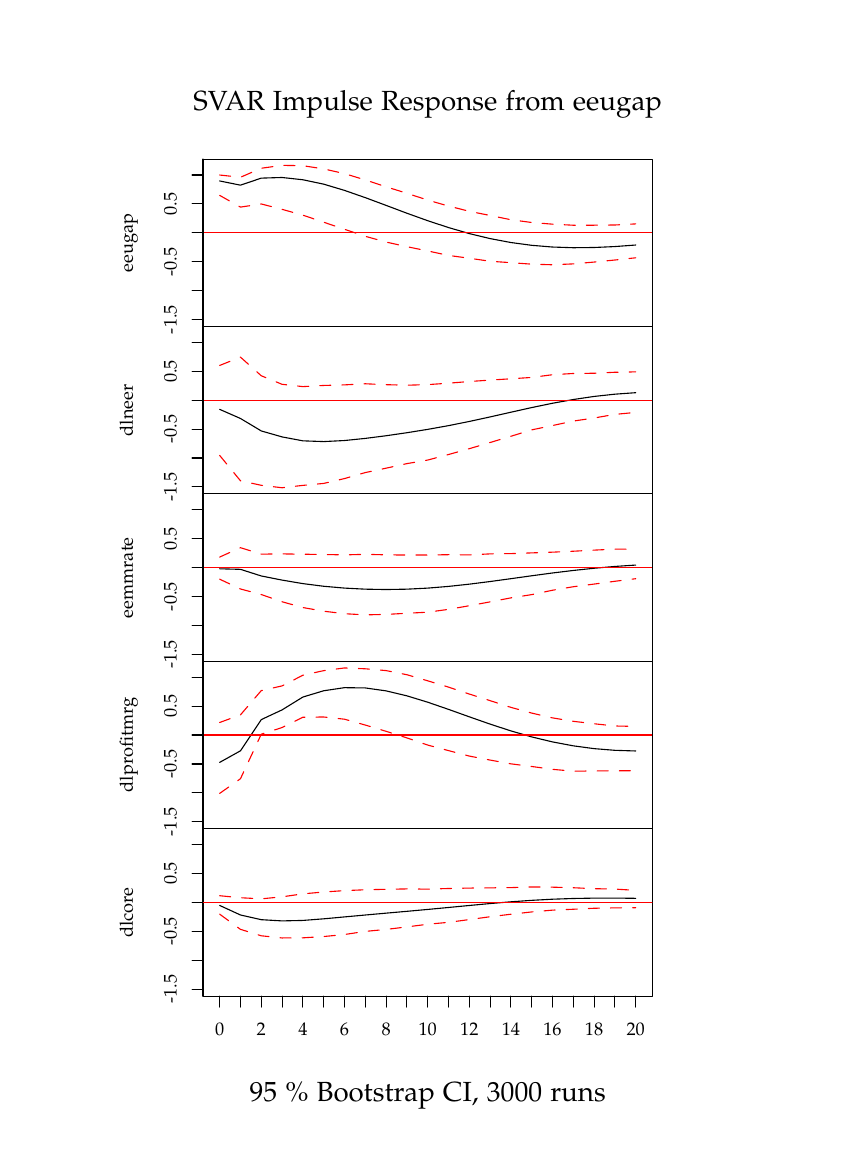
\begin{tikzpicture}[x=1pt,y=1pt]
\definecolor{fillColor}{RGB}{255,255,255}
\path[use as bounding box,fill=fillColor,fill opacity=0.00] (0,0) rectangle (289.08,397.48);
\begin{scope}
\path[clip] ( 63.36,289.48) rectangle (225.72,349.96);
\definecolor{drawColor}{RGB}{0,0,0}

\path[draw=drawColor,line width= 0.4pt,line join=round,line cap=round] ( 69.37,342.09) --
	( 76.89,340.56) --
	( 84.41,343.11) --
	( 91.92,343.34) --
	( 99.44,342.52) --
	(106.96,340.93) --
	(114.47,338.68) --
	(121.99,336.06) --
	(129.51,333.26) --
	(137.02,330.43) --
	(144.54,327.73) --
	(152.06,325.25) --
	(159.57,323.07) --
	(167.09,321.26) --
	(174.61,319.84) --
	(182.12,318.83) --
	(189.64,318.21) --
	(197.16,317.96) --
	(204.67,318.04) --
	(212.19,318.38) --
	(219.71,318.94);
\end{scope}
\begin{scope}
\path[clip] ( 31.68,289.48) rectangle (257.40,349.96);
\definecolor{drawColor}{RGB}{0,0,0}

\node[text=drawColor,anchor=base,inner sep=0pt, outer sep=0pt, scale=  0.66] at (144.54,259.38) {xy{\$}x};

\node[text=drawColor,rotate= 90.00,anchor=base,inner sep=0pt, outer sep=0pt, scale=  0.66] at ( 38.02,319.72) {eeugap};
\end{scope}
\begin{scope}
\path[clip] (  0.00,  0.00) rectangle (289.08,397.48);
\definecolor{drawColor}{RGB}{0,0,0}

\path[draw=drawColor,line width= 0.4pt,line join=round,line cap=round] ( 63.36,292.01) -- ( 63.36,349.97);

\path[draw=drawColor,line width= 0.4pt,line join=round,line cap=round] ( 63.36,292.01) -- ( 59.40,292.01);

\path[draw=drawColor,line width= 0.4pt,line join=round,line cap=round] ( 63.36,302.45) -- ( 59.40,302.45);

\path[draw=drawColor,line width= 0.4pt,line join=round,line cap=round] ( 63.36,312.89) -- ( 59.40,312.89);

\path[draw=drawColor,line width= 0.4pt,line join=round,line cap=round] ( 63.36,323.33) -- ( 59.40,323.33);

\path[draw=drawColor,line width= 0.4pt,line join=round,line cap=round] ( 63.36,333.78) -- ( 59.40,333.78);

\path[draw=drawColor,line width= 0.4pt,line join=round,line cap=round] ( 63.36,344.22) -- ( 59.40,344.22);

\node[text=drawColor,rotate= 90.00,anchor=base,inner sep=0pt, outer sep=0pt, scale=  0.66] at ( 53.86,292.01) {-1.5};

\node[text=drawColor,rotate= 90.00,anchor=base,inner sep=0pt, outer sep=0pt, scale=  0.66] at ( 53.86,312.89) {-0.5};

\node[text=drawColor,rotate= 90.00,anchor=base,inner sep=0pt, outer sep=0pt, scale=  0.66] at ( 53.86,333.78) {0.5};
\end{scope}
\begin{scope}
\path[clip] ( 63.36,289.48) rectangle (225.72,349.96);
\definecolor{drawColor}{RGB}{255,0,0}

\path[draw=drawColor,line width= 0.4pt,line join=round,line cap=round] ( 63.36,323.33) -- (225.72,323.33);

\path[draw=drawColor,line width= 0.4pt,dash pattern=on 4pt off 4pt ,line join=round,line cap=round] ( 69.37,344.23) --
	( 76.89,343.42) --
	( 84.41,346.68) --
	( 91.92,347.72) --
	( 99.44,347.60) --
	(106.96,346.44) --
	(114.47,344.74) --
	(121.99,342.46) --
	(129.51,339.98) --
	(137.02,337.64) --
	(144.54,335.17) --
	(152.06,333.02) --
	(159.57,331.13) --
	(167.09,329.61) --
	(174.61,328.08) --
	(182.12,327.08) --
	(189.64,326.47) --
	(197.16,326.09) --
	(204.67,326.10) --
	(212.19,326.17) --
	(219.71,326.57);

\path[draw=drawColor,line width= 0.4pt,dash pattern=on 4pt off 4pt ,line join=round,line cap=round] ( 69.37,336.88) --
	( 76.89,332.64) --
	( 84.41,333.77) --
	( 91.92,331.83) --
	( 99.44,329.73) --
	(106.96,327.18) --
	(114.47,324.64) --
	(121.99,322.09) --
	(129.51,320.01) --
	(137.02,318.34) --
	(144.54,316.80) --
	(152.06,315.18) --
	(159.57,314.16) --
	(167.09,313.07) --
	(174.61,312.56) --
	(182.12,312.02) --
	(189.64,311.80) --
	(197.16,312.12) --
	(204.67,312.78) --
	(212.19,313.52) --
	(219.71,314.32);
\end{scope}
\begin{scope}
\path[clip] (  0.00,  0.00) rectangle (289.08,397.48);
\definecolor{drawColor}{RGB}{0,0,0}

\path[draw=drawColor,line width= 0.4pt,line join=round,line cap=round] ( 63.36,289.48) --
	(225.72,289.48) --
	(225.72,349.96) --
	( 63.36,349.96) --
	( 63.36,289.48);
\end{scope}
\begin{scope}
\path[clip] ( 63.36,228.99) rectangle (225.72,289.48);
\definecolor{drawColor}{RGB}{0,0,0}

\path[draw=drawColor,line width= 0.4pt,line join=round,line cap=round] ( 69.37,259.56) --
	( 76.89,256.26) --
	( 84.41,251.75) --
	( 91.92,249.60) --
	( 99.44,248.18) --
	(106.96,247.91) --
	(114.47,248.29) --
	(121.99,249.06) --
	(129.51,250.02) --
	(137.02,251.11) --
	(144.54,252.32) --
	(152.06,253.67) --
	(159.57,255.18) --
	(167.09,256.82) --
	(174.61,258.52) --
	(182.12,260.20) --
	(189.64,261.76) --
	(197.16,263.11) --
	(204.67,264.22) --
	(212.19,265.04) --
	(219.71,265.58);
\end{scope}
\begin{scope}
\path[clip] ( 31.68,228.99) rectangle (257.40,289.48);
\definecolor{drawColor}{RGB}{0,0,0}

\node[text=drawColor,anchor=base,inner sep=0pt, outer sep=0pt, scale=  0.66] at (144.54,198.89) {xy{\$}x};

\node[text=drawColor,rotate= 90.00,anchor=base,inner sep=0pt, outer sep=0pt, scale=  0.66] at ( 38.02,259.23) {dlneer};
\end{scope}
\begin{scope}
\path[clip] (  0.00,  0.00) rectangle (289.08,397.48);
\definecolor{drawColor}{RGB}{0,0,0}

\path[draw=drawColor,line width= 0.4pt,line join=round,line cap=round] ( 63.36,231.52) -- ( 63.36,289.48);

\path[draw=drawColor,line width= 0.4pt,line join=round,line cap=round] ( 63.36,231.52) -- ( 59.40,231.52);

\path[draw=drawColor,line width= 0.4pt,line join=round,line cap=round] ( 63.36,241.96) -- ( 59.40,241.96);

\path[draw=drawColor,line width= 0.4pt,line join=round,line cap=round] ( 63.36,252.40) -- ( 59.40,252.40);

\path[draw=drawColor,line width= 0.4pt,line join=round,line cap=round] ( 63.36,262.85) -- ( 59.40,262.85);

\path[draw=drawColor,line width= 0.4pt,line join=round,line cap=round] ( 63.36,273.29) -- ( 59.40,273.29);

\path[draw=drawColor,line width= 0.4pt,line join=round,line cap=round] ( 63.36,283.73) -- ( 59.40,283.73);

\node[text=drawColor,rotate= 90.00,anchor=base,inner sep=0pt, outer sep=0pt, scale=  0.66] at ( 53.86,231.52) {-1.5};

\node[text=drawColor,rotate= 90.00,anchor=base,inner sep=0pt, outer sep=0pt, scale=  0.66] at ( 53.86,252.40) {-0.5};

\node[text=drawColor,rotate= 90.00,anchor=base,inner sep=0pt, outer sep=0pt, scale=  0.66] at ( 53.86,273.29) {0.5};
\end{scope}
\begin{scope}
\path[clip] ( 63.36,228.99) rectangle (225.72,289.48);
\definecolor{drawColor}{RGB}{255,0,0}

\path[draw=drawColor,line width= 0.4pt,line join=round,line cap=round] ( 63.36,262.85) -- (225.72,262.85);

\path[draw=drawColor,line width= 0.4pt,dash pattern=on 4pt off 4pt ,line join=round,line cap=round] ( 69.37,275.42) --
	( 76.89,278.43) --
	( 84.41,271.69) --
	( 91.92,268.61) --
	( 99.44,267.77) --
	(106.96,268.19) --
	(114.47,268.40) --
	(121.99,268.80) --
	(129.51,268.47) --
	(137.02,268.28) --
	(144.54,268.49) --
	(152.06,269.01) --
	(159.57,269.61) --
	(167.09,270.13) --
	(174.61,270.60) --
	(182.12,271.09) --
	(189.64,272.07) --
	(197.16,272.52) --
	(204.67,272.60) --
	(212.19,272.96) --
	(219.71,273.10);

\path[draw=drawColor,line width= 0.4pt,dash pattern=on 4pt off 4pt ,line join=round,line cap=round] ( 69.37,242.92) --
	( 76.89,233.75) --
	( 84.41,232.11) --
	( 91.92,231.23) --
	( 99.44,232.08) --
	(106.96,232.79) --
	(114.47,234.54) --
	(121.99,236.71) --
	(129.51,238.30) --
	(137.02,239.95) --
	(144.54,241.23) --
	(152.06,243.23) --
	(159.57,245.34) --
	(167.09,247.57) --
	(174.61,249.83) --
	(182.12,252.14) --
	(189.64,253.71) --
	(197.16,255.32) --
	(204.67,256.43) --
	(212.19,257.74) --
	(219.71,258.45);
\end{scope}
\begin{scope}
\path[clip] (  0.00,  0.00) rectangle (289.08,397.48);
\definecolor{drawColor}{RGB}{0,0,0}

\path[draw=drawColor,line width= 0.4pt,line join=round,line cap=round] ( 63.36,228.99) --
	(225.72,228.99) --
	(225.72,289.48) --
	( 63.36,289.48) --
	( 63.36,228.99);
\end{scope}
\begin{scope}
\path[clip] ( 63.36,168.50) rectangle (225.72,228.99);
\definecolor{drawColor}{RGB}{0,0,0}

\path[draw=drawColor,line width= 0.4pt,line join=round,line cap=round] ( 69.37,201.94) --
	( 76.89,201.75) --
	( 84.41,199.35) --
	( 91.92,197.86) --
	( 99.44,196.59) --
	(106.96,195.63) --
	(114.47,194.97) --
	(121.99,194.58) --
	(129.51,194.45) --
	(137.02,194.58) --
	(144.54,194.96) --
	(152.06,195.58) --
	(159.57,196.39) --
	(167.09,197.34) --
	(174.61,198.37) --
	(182.12,199.42) --
	(189.64,200.43) --
	(197.16,201.34) --
	(204.67,202.14) --
	(212.19,202.79) --
	(219.71,203.29);
\end{scope}
\begin{scope}
\path[clip] ( 31.68,168.50) rectangle (257.40,228.99);
\definecolor{drawColor}{RGB}{0,0,0}

\node[text=drawColor,anchor=base,inner sep=0pt, outer sep=0pt, scale=  0.66] at (144.54,138.40) {xy{\$}x};

\node[text=drawColor,rotate= 90.00,anchor=base,inner sep=0pt, outer sep=0pt, scale=  0.66] at ( 38.02,198.74) {eemmrate};
\end{scope}
\begin{scope}
\path[clip] (  0.00,  0.00) rectangle (289.08,397.48);
\definecolor{drawColor}{RGB}{0,0,0}

\path[draw=drawColor,line width= 0.4pt,line join=round,line cap=round] ( 63.36,171.03) -- ( 63.36,228.99);

\path[draw=drawColor,line width= 0.4pt,line join=round,line cap=round] ( 63.36,171.03) -- ( 59.40,171.03);

\path[draw=drawColor,line width= 0.4pt,line join=round,line cap=round] ( 63.36,181.47) -- ( 59.40,181.47);

\path[draw=drawColor,line width= 0.4pt,line join=round,line cap=round] ( 63.36,191.91) -- ( 59.40,191.91);

\path[draw=drawColor,line width= 0.4pt,line join=round,line cap=round] ( 63.36,202.36) -- ( 59.40,202.36);

\path[draw=drawColor,line width= 0.4pt,line join=round,line cap=round] ( 63.36,212.80) -- ( 59.40,212.80);

\path[draw=drawColor,line width= 0.4pt,line join=round,line cap=round] ( 63.36,223.24) -- ( 59.40,223.24);

\node[text=drawColor,rotate= 90.00,anchor=base,inner sep=0pt, outer sep=0pt, scale=  0.66] at ( 53.86,171.03) {-1.5};

\node[text=drawColor,rotate= 90.00,anchor=base,inner sep=0pt, outer sep=0pt, scale=  0.66] at ( 53.86,191.91) {-0.5};

\node[text=drawColor,rotate= 90.00,anchor=base,inner sep=0pt, outer sep=0pt, scale=  0.66] at ( 53.86,212.80) {0.5};
\end{scope}
\begin{scope}
\path[clip] ( 63.36,168.50) rectangle (225.72,228.99);
\definecolor{drawColor}{RGB}{255,0,0}

\path[draw=drawColor,line width= 0.4pt,line join=round,line cap=round] ( 63.36,202.36) -- (225.72,202.36);

\path[draw=drawColor,line width= 0.4pt,dash pattern=on 4pt off 4pt ,line join=round,line cap=round] ( 69.37,206.18) --
	( 76.89,209.57) --
	( 84.41,207.24) --
	( 91.92,207.33) --
	( 99.44,207.21) --
	(106.96,207.11) --
	(114.47,206.97) --
	(121.99,207.17) --
	(129.51,206.99) --
	(137.02,206.90) --
	(144.54,206.92) --
	(152.06,207.04) --
	(159.57,206.96) --
	(167.09,207.33) --
	(174.61,207.43) --
	(182.12,207.69) --
	(189.64,207.95) --
	(197.16,208.29) --
	(204.67,208.69) --
	(212.19,209.04) --
	(219.71,209.02);

\path[draw=drawColor,line width= 0.4pt,dash pattern=on 4pt off 4pt ,line join=round,line cap=round] ( 69.37,198.19) --
	( 76.89,194.65) --
	( 84.41,192.64) --
	( 91.92,190.03) --
	( 99.44,187.94) --
	(106.96,186.62) --
	(114.47,185.71) --
	(121.99,185.30) --
	(129.51,185.46) --
	(137.02,185.87) --
	(144.54,186.26) --
	(152.06,187.28) --
	(159.57,188.59) --
	(167.09,189.99) --
	(174.61,191.44) --
	(182.12,192.61) --
	(189.64,194.19) --
	(197.16,195.46) --
	(204.67,196.42) --
	(212.19,197.43) --
	(219.71,198.36);
\end{scope}
\begin{scope}
\path[clip] (  0.00,  0.00) rectangle (289.08,397.48);
\definecolor{drawColor}{RGB}{0,0,0}

\path[draw=drawColor,line width= 0.4pt,line join=round,line cap=round] ( 63.36,168.50) --
	(225.72,168.50) --
	(225.72,228.99) --
	( 63.36,228.99) --
	( 63.36,168.50);
\end{scope}
\begin{scope}
\path[clip] ( 63.36,108.01) rectangle (225.72,168.50);
\definecolor{drawColor}{RGB}{0,0,0}

\path[draw=drawColor,line width= 0.4pt,line join=round,line cap=round] ( 69.37,131.98) --
	( 76.89,136.17) --
	( 84.41,147.45) --
	( 91.92,150.96) --
	( 99.44,155.60) --
	(106.96,157.87) --
	(114.47,158.99) --
	(121.99,158.89) --
	(129.51,157.83) --
	(137.02,156.04) --
	(144.54,153.74) --
	(152.06,151.15) --
	(159.57,148.46) --
	(167.09,145.82) --
	(174.61,143.37) --
	(182.12,141.20) --
	(189.64,139.39) --
	(197.16,137.97) --
	(204.67,136.96) --
	(212.19,136.35) --
	(219.71,136.11);
\end{scope}
\begin{scope}
\path[clip] ( 31.68,108.01) rectangle (257.40,168.50);
\definecolor{drawColor}{RGB}{0,0,0}

\node[text=drawColor,anchor=base,inner sep=0pt, outer sep=0pt, scale=  0.66] at (144.54, 77.91) {xy{\$}x};

\node[text=drawColor,rotate= 90.00,anchor=base,inner sep=0pt, outer sep=0pt, scale=  0.66] at ( 38.02,138.25) {dlprofitmrg};
\end{scope}
\begin{scope}
\path[clip] (  0.00,  0.00) rectangle (289.08,397.48);
\definecolor{drawColor}{RGB}{0,0,0}

\path[draw=drawColor,line width= 0.4pt,line join=round,line cap=round] ( 63.36,110.54) -- ( 63.36,168.50);

\path[draw=drawColor,line width= 0.4pt,line join=round,line cap=round] ( 63.36,110.54) -- ( 59.40,110.54);

\path[draw=drawColor,line width= 0.4pt,line join=round,line cap=round] ( 63.36,120.98) -- ( 59.40,120.98);

\path[draw=drawColor,line width= 0.4pt,line join=round,line cap=round] ( 63.36,131.42) -- ( 59.40,131.42);

\path[draw=drawColor,line width= 0.4pt,line join=round,line cap=round] ( 63.36,141.87) -- ( 59.40,141.87);

\path[draw=drawColor,line width= 0.4pt,line join=round,line cap=round] ( 63.36,152.31) -- ( 59.40,152.31);

\path[draw=drawColor,line width= 0.4pt,line join=round,line cap=round] ( 63.36,162.75) -- ( 59.40,162.75);

\node[text=drawColor,rotate= 90.00,anchor=base,inner sep=0pt, outer sep=0pt, scale=  0.66] at ( 53.86,110.54) {-1.5};

\node[text=drawColor,rotate= 90.00,anchor=base,inner sep=0pt, outer sep=0pt, scale=  0.66] at ( 53.86,131.42) {-0.5};

\node[text=drawColor,rotate= 90.00,anchor=base,inner sep=0pt, outer sep=0pt, scale=  0.66] at ( 53.86,152.31) {0.5};
\end{scope}
\begin{scope}
\path[clip] ( 63.36,108.01) rectangle (225.72,168.50);
\definecolor{drawColor}{RGB}{255,0,0}

\path[draw=drawColor,line width= 0.4pt,line join=round,line cap=round] ( 63.36,141.87) -- (225.72,141.87);

\path[draw=drawColor,line width= 0.4pt,dash pattern=on 4pt off 4pt ,line join=round,line cap=round] ( 69.37,146.40) --
	( 76.89,149.16) --
	( 84.41,157.93) --
	( 91.92,159.63) --
	( 99.44,163.48) --
	(106.96,165.14) --
	(114.47,166.11) --
	(121.99,165.81) --
	(129.51,165.16) --
	(137.02,163.67) --
	(144.54,161.47) --
	(152.06,159.20) --
	(159.57,156.69) --
	(167.09,154.30) --
	(174.61,151.87) --
	(182.12,149.81) --
	(189.64,148.07) --
	(197.16,146.83) --
	(204.67,145.95) --
	(212.19,145.14) --
	(219.71,144.99);

\path[draw=drawColor,line width= 0.4pt,dash pattern=on 4pt off 4pt ,line join=round,line cap=round] ( 69.37,120.78) --
	( 76.89,126.08) --
	( 84.41,142.17) --
	( 91.92,144.57) --
	( 99.44,148.31) --
	(106.96,148.39) --
	(114.47,147.60) --
	(121.99,145.48) --
	(129.51,143.22) --
	(137.02,140.84) --
	(144.54,138.25) --
	(152.06,136.25) --
	(159.57,134.27) --
	(167.09,132.83) --
	(174.61,131.46) --
	(182.12,130.51) --
	(189.64,129.48) --
	(197.16,128.80) --
	(204.67,128.90) --
	(212.19,128.95) --
	(219.71,128.96);
\end{scope}
\begin{scope}
\path[clip] (  0.00,  0.00) rectangle (289.08,397.48);
\definecolor{drawColor}{RGB}{0,0,0}

\path[draw=drawColor,line width= 0.4pt,line join=round,line cap=round] ( 63.36,108.01) --
	(225.72,108.01) --
	(225.72,168.50) --
	( 63.36,168.50) --
	( 63.36,108.01);
\end{scope}
\begin{scope}
\path[clip] ( 63.36, 47.52) rectangle (225.72,108.01);
\definecolor{drawColor}{RGB}{0,0,0}

\path[draw=drawColor,line width= 0.4pt,line join=round,line cap=round] ( 69.37, 80.30) --
	( 76.89, 76.85) --
	( 84.41, 75.15) --
	( 91.92, 74.71) --
	( 99.44, 74.88) --
	(106.96, 75.46) --
	(114.47, 76.15) --
	(121.99, 76.84) --
	(129.51, 77.51) --
	(137.02, 78.17) --
	(144.54, 78.85) --
	(152.06, 79.56) --
	(159.57, 80.28) --
	(167.09, 80.98) --
	(174.61, 81.61) --
	(182.12, 82.14) --
	(189.64, 82.55) --
	(197.16, 82.81) --
	(204.67, 82.94) --
	(212.19, 82.96) --
	(219.71, 82.87);
\end{scope}
\begin{scope}
\path[clip] ( 31.68, 47.52) rectangle (257.40,108.01);
\definecolor{drawColor}{RGB}{0,0,0}

\node[text=drawColor,anchor=base,inner sep=0pt, outer sep=0pt, scale=  0.66] at (144.54, 17.42) {xy{\$}x};

\node[text=drawColor,rotate= 90.00,anchor=base,inner sep=0pt, outer sep=0pt, scale=  0.66] at ( 38.02, 77.76) {dlcore};
\end{scope}
\begin{scope}
\path[clip] (  0.00,  0.00) rectangle (289.08,397.48);
\definecolor{drawColor}{RGB}{0,0,0}

\path[draw=drawColor,line width= 0.4pt,line join=round,line cap=round] ( 63.36, 50.05) -- ( 63.36,108.01);

\path[draw=drawColor,line width= 0.4pt,line join=round,line cap=round] ( 63.36, 50.05) -- ( 59.40, 50.05);

\path[draw=drawColor,line width= 0.4pt,line join=round,line cap=round] ( 63.36, 60.49) -- ( 59.40, 60.49);

\path[draw=drawColor,line width= 0.4pt,line join=round,line cap=round] ( 63.36, 70.94) -- ( 59.40, 70.94);

\path[draw=drawColor,line width= 0.4pt,line join=round,line cap=round] ( 63.36, 81.38) -- ( 59.40, 81.38);

\path[draw=drawColor,line width= 0.4pt,line join=round,line cap=round] ( 63.36, 91.82) -- ( 59.40, 91.82);

\path[draw=drawColor,line width= 0.4pt,line join=round,line cap=round] ( 63.36,102.26) -- ( 59.40,102.26);

\node[text=drawColor,rotate= 90.00,anchor=base,inner sep=0pt, outer sep=0pt, scale=  0.66] at ( 53.86, 50.05) {-1.5};

\node[text=drawColor,rotate= 90.00,anchor=base,inner sep=0pt, outer sep=0pt, scale=  0.66] at ( 53.86, 70.94) {-0.5};

\node[text=drawColor,rotate= 90.00,anchor=base,inner sep=0pt, outer sep=0pt, scale=  0.66] at ( 53.86, 91.82) {0.5};

\path[draw=drawColor,line width= 0.4pt,line join=round,line cap=round] ( 69.37, 47.52) -- (219.71, 47.52);

\path[draw=drawColor,line width= 0.4pt,line join=round,line cap=round] ( 69.37, 47.52) -- ( 69.37, 43.56);

\path[draw=drawColor,line width= 0.4pt,line join=round,line cap=round] ( 76.89, 47.52) -- ( 76.89, 43.56);

\path[draw=drawColor,line width= 0.4pt,line join=round,line cap=round] ( 84.41, 47.52) -- ( 84.41, 43.56);

\path[draw=drawColor,line width= 0.4pt,line join=round,line cap=round] ( 91.92, 47.52) -- ( 91.92, 43.56);

\path[draw=drawColor,line width= 0.4pt,line join=round,line cap=round] ( 99.44, 47.52) -- ( 99.44, 43.56);

\path[draw=drawColor,line width= 0.4pt,line join=round,line cap=round] (106.96, 47.52) -- (106.96, 43.56);

\path[draw=drawColor,line width= 0.4pt,line join=round,line cap=round] (114.47, 47.52) -- (114.47, 43.56);

\path[draw=drawColor,line width= 0.4pt,line join=round,line cap=round] (121.99, 47.52) -- (121.99, 43.56);

\path[draw=drawColor,line width= 0.4pt,line join=round,line cap=round] (129.51, 47.52) -- (129.51, 43.56);

\path[draw=drawColor,line width= 0.4pt,line join=round,line cap=round] (137.02, 47.52) -- (137.02, 43.56);

\path[draw=drawColor,line width= 0.4pt,line join=round,line cap=round] (144.54, 47.52) -- (144.54, 43.56);

\path[draw=drawColor,line width= 0.4pt,line join=round,line cap=round] (152.06, 47.52) -- (152.06, 43.56);

\path[draw=drawColor,line width= 0.4pt,line join=round,line cap=round] (159.57, 47.52) -- (159.57, 43.56);

\path[draw=drawColor,line width= 0.4pt,line join=round,line cap=round] (167.09, 47.52) -- (167.09, 43.56);

\path[draw=drawColor,line width= 0.4pt,line join=round,line cap=round] (174.61, 47.52) -- (174.61, 43.56);

\path[draw=drawColor,line width= 0.4pt,line join=round,line cap=round] (182.12, 47.52) -- (182.12, 43.56);

\path[draw=drawColor,line width= 0.4pt,line join=round,line cap=round] (189.64, 47.52) -- (189.64, 43.56);

\path[draw=drawColor,line width= 0.4pt,line join=round,line cap=round] (197.16, 47.52) -- (197.16, 43.56);

\path[draw=drawColor,line width= 0.4pt,line join=round,line cap=round] (204.67, 47.52) -- (204.67, 43.56);

\path[draw=drawColor,line width= 0.4pt,line join=round,line cap=round] (212.19, 47.52) -- (212.19, 43.56);

\path[draw=drawColor,line width= 0.4pt,line join=round,line cap=round] (219.71, 47.52) -- (219.71, 43.56);

\node[text=drawColor,anchor=base,inner sep=0pt, outer sep=0pt, scale=  0.66] at ( 69.37, 33.26) {0};

\node[text=drawColor,anchor=base,inner sep=0pt, outer sep=0pt, scale=  0.66] at ( 84.41, 33.26) {2};

\node[text=drawColor,anchor=base,inner sep=0pt, outer sep=0pt, scale=  0.66] at ( 99.44, 33.26) {4};

\node[text=drawColor,anchor=base,inner sep=0pt, outer sep=0pt, scale=  0.66] at (114.47, 33.26) {6};

\node[text=drawColor,anchor=base,inner sep=0pt, outer sep=0pt, scale=  0.66] at (129.51, 33.26) {8};

\node[text=drawColor,anchor=base,inner sep=0pt, outer sep=0pt, scale=  0.66] at (144.54, 33.26) {10};

\node[text=drawColor,anchor=base,inner sep=0pt, outer sep=0pt, scale=  0.66] at (159.57, 33.26) {12};

\node[text=drawColor,anchor=base,inner sep=0pt, outer sep=0pt, scale=  0.66] at (174.61, 33.26) {14};

\node[text=drawColor,anchor=base,inner sep=0pt, outer sep=0pt, scale=  0.66] at (189.64, 33.26) {16};

\node[text=drawColor,anchor=base,inner sep=0pt, outer sep=0pt, scale=  0.66] at (204.67, 33.26) {18};

\node[text=drawColor,anchor=base,inner sep=0pt, outer sep=0pt, scale=  0.66] at (219.71, 33.26) {20};

\path[draw=drawColor,line width= 0.4pt,line join=round,line cap=round] ( 63.36, 47.52) --
	(225.72, 47.52) --
	(225.72,108.01) --
	( 63.36,108.01) --
	( 63.36, 47.52);
\end{scope}
\begin{scope}
\path[clip] ( 63.36, 47.52) rectangle (225.72,108.01);
\definecolor{drawColor}{RGB}{255,0,0}

\path[draw=drawColor,line width= 0.4pt,line join=round,line cap=round] ( 63.36, 81.38) -- (225.72, 81.38);

\path[draw=drawColor,line width= 0.4pt,dash pattern=on 4pt off 4pt ,line join=round,line cap=round] ( 69.37, 83.81) --
	( 76.89, 83.08) --
	( 84.41, 82.68) --
	( 91.92, 83.41) --
	( 99.44, 84.48) --
	(106.96, 85.16) --
	(114.47, 85.65) --
	(121.99, 85.96) --
	(129.51, 86.13) --
	(137.02, 86.27) --
	(144.54, 86.19) --
	(152.06, 86.42) --
	(159.57, 86.57) --
	(167.09, 86.65) --
	(174.61, 86.74) --
	(182.12, 86.98) --
	(189.64, 86.90) --
	(197.16, 86.69) --
	(204.67, 86.36) --
	(212.19, 86.20) --
	(219.71, 85.76);

\path[draw=drawColor,line width= 0.4pt,dash pattern=on 4pt off 4pt ,line join=round,line cap=round] ( 69.37, 77.15) --
	( 76.89, 71.66) --
	( 84.41, 69.33) --
	( 91.92, 68.55) --
	( 99.44, 68.59) --
	(106.96, 69.06) --
	(114.47, 69.79) --
	(121.99, 70.92) --
	(129.51, 71.63) --
	(137.02, 72.54) --
	(144.54, 73.50) --
	(152.06, 74.19) --
	(159.57, 75.19) --
	(167.09, 76.21) --
	(174.61, 77.12) --
	(182.12, 77.95) --
	(189.64, 78.60) --
	(197.16, 78.92) --
	(204.67, 79.28) --
	(212.19, 79.42) --
	(219.71, 79.48);
\end{scope}
\begin{scope}
\path[clip] (  0.00,  0.00) rectangle (289.08,397.48);
\definecolor{drawColor}{RGB}{0,0,0}

\node[text=drawColor,anchor=base,inner sep=0pt, outer sep=0pt, scale=  1.00] at (144.54,367.39) {SVAR Impulse Response from eeugap};

\node[text=drawColor,anchor=base,inner sep=0pt, outer sep=0pt, scale=  1.00] at (144.54,  9.50) {95 {\%} Bootstrap CI,  3000 runs};
\end{scope}
\end{tikzpicture}
}
\vspace*{-10mm}
\caption{Impulse response to unemployment gap shock in VAR}\label{fig:IRS_eeugap}
% \vspace*{-4mm} %get rid of the nas
% \caption*{Source: EUROSTAT  (namq\_10\_gdp, namq\_10\_lp\_ulc)}
\end{figure}

\begin{figure}[H]
% \centering
\resizebox{12 cm}{!}{% Created by tikzDevice version 0.9 on 2016-01-13 23:40:06
% !TEX encoding = UTF-8 Unicode
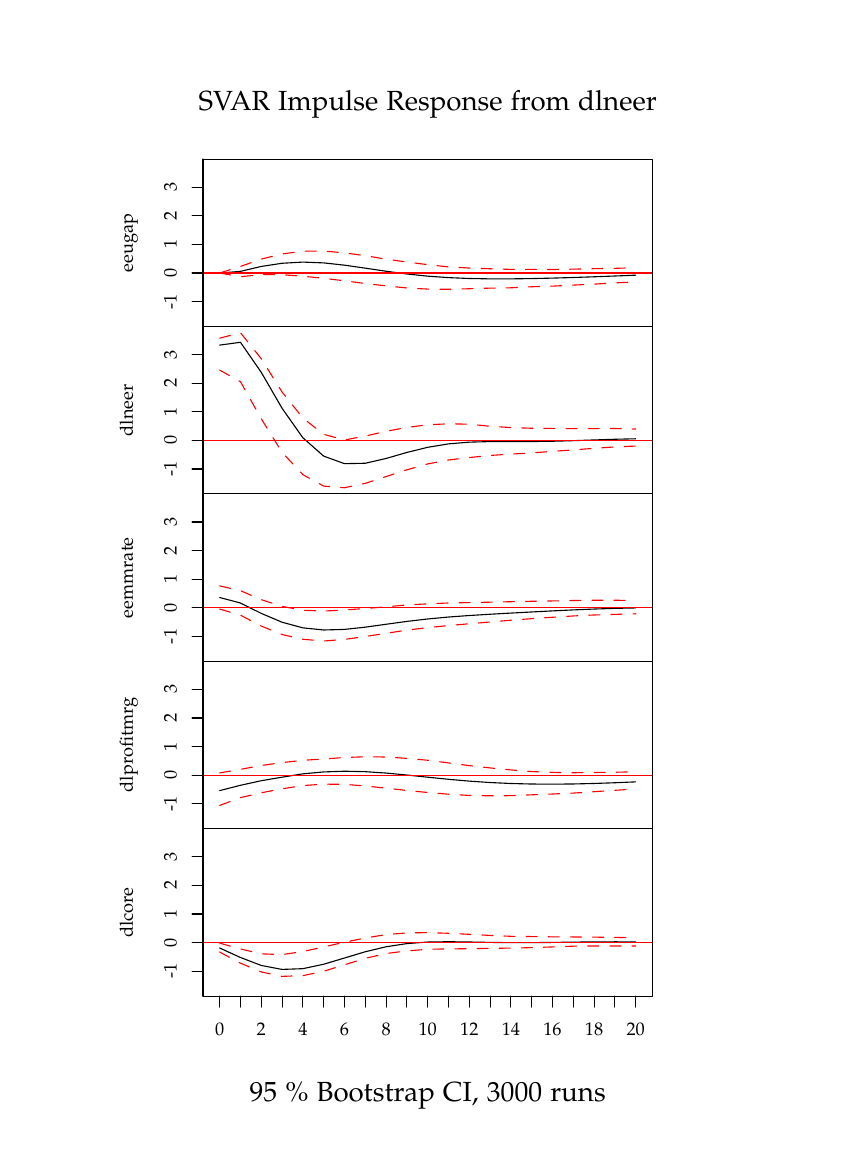
\begin{tikzpicture}[x=1pt,y=1pt]
\definecolor{fillColor}{RGB}{255,255,255}
\path[use as bounding box,fill=fillColor,fill opacity=0.00] (0,0) rectangle (289.08,397.48);
\begin{scope}
\path[clip] ( 63.36,289.48) rectangle (225.72,349.96);
\definecolor{drawColor}{RGB}{0,0,0}

\path[draw=drawColor,line width= 0.4pt,line join=round,line cap=round] ( 69.37,308.82) --
	( 76.89,309.41) --
	( 84.41,311.20) --
	( 91.92,312.34) --
	( 99.44,312.77) --
	(106.96,312.48) --
	(114.47,311.66) --
	(121.99,310.58) --
	(129.51,309.46) --
	(137.02,308.47) --
	(144.54,307.69) --
	(152.06,307.16) --
	(159.57,306.84) --
	(167.09,306.71) --
	(174.61,306.71) --
	(182.12,306.81) --
	(189.64,306.98) --
	(197.16,307.20) --
	(204.67,307.46) --
	(212.19,307.74) --
	(219.71,308.04);
\end{scope}
\begin{scope}
\path[clip] ( 31.68,289.48) rectangle (257.40,349.96);
\definecolor{drawColor}{RGB}{0,0,0}

\node[text=drawColor,anchor=base,inner sep=0pt, outer sep=0pt, scale=  0.66] at (144.54,259.38) {xy{\$}x};

\node[text=drawColor,rotate= 90.00,anchor=base,inner sep=0pt, outer sep=0pt, scale=  0.66] at ( 38.02,319.72) {eeugap};
\end{scope}
\begin{scope}
\path[clip] (  0.00,  0.00) rectangle (289.08,397.48);
\definecolor{drawColor}{RGB}{0,0,0}

\path[draw=drawColor,line width= 0.4pt,line join=round,line cap=round] ( 63.36,298.49) -- ( 63.36,349.97);

\path[draw=drawColor,line width= 0.4pt,line join=round,line cap=round] ( 63.36,298.49) -- ( 59.40,298.49);

\path[draw=drawColor,line width= 0.4pt,line join=round,line cap=round] ( 63.36,308.82) -- ( 59.40,308.82);

\path[draw=drawColor,line width= 0.4pt,line join=round,line cap=round] ( 63.36,319.16) -- ( 59.40,319.16);

\path[draw=drawColor,line width= 0.4pt,line join=round,line cap=round] ( 63.36,329.49) -- ( 59.40,329.49);

\path[draw=drawColor,line width= 0.4pt,line join=round,line cap=round] ( 63.36,339.83) -- ( 59.40,339.83);

\node[text=drawColor,rotate= 90.00,anchor=base,inner sep=0pt, outer sep=0pt, scale=  0.66] at ( 53.86,298.49) {-1};

\node[text=drawColor,rotate= 90.00,anchor=base,inner sep=0pt, outer sep=0pt, scale=  0.66] at ( 53.86,308.82) {0};

\node[text=drawColor,rotate= 90.00,anchor=base,inner sep=0pt, outer sep=0pt, scale=  0.66] at ( 53.86,319.16) {1};

\node[text=drawColor,rotate= 90.00,anchor=base,inner sep=0pt, outer sep=0pt, scale=  0.66] at ( 53.86,329.49) {2};

\node[text=drawColor,rotate= 90.00,anchor=base,inner sep=0pt, outer sep=0pt, scale=  0.66] at ( 53.86,339.83) {3};
\end{scope}
\begin{scope}
\path[clip] ( 63.36,289.48) rectangle (225.72,349.96);
\definecolor{drawColor}{RGB}{255,0,0}

\path[draw=drawColor,line width= 0.4pt,line join=round,line cap=round] ( 63.36,308.82) -- (225.72,308.82);

\path[draw=drawColor,line width= 0.4pt,dash pattern=on 4pt off 4pt ,line join=round,line cap=round] ( 69.37,308.82) --
	( 76.89,311.21) --
	( 84.41,313.85) --
	( 91.92,315.72) --
	( 99.44,316.70) --
	(106.96,316.78) --
	(114.47,316.10) --
	(121.99,315.09) --
	(129.51,313.83) --
	(137.02,312.79) --
	(144.54,311.85) --
	(152.06,311.03) --
	(159.57,310.62) --
	(167.09,310.36) --
	(174.61,310.13) --
	(182.12,310.12) --
	(189.64,310.09) --
	(197.16,310.22) --
	(204.67,310.39) --
	(212.19,310.51) --
	(219.71,310.74);

\path[draw=drawColor,line width= 0.4pt,dash pattern=on 4pt off 4pt ,line join=round,line cap=round] ( 69.37,308.82) --
	( 76.89,307.48) --
	( 84.41,308.24) --
	( 91.92,308.21) --
	( 99.44,307.66) --
	(106.96,306.92) --
	(114.47,306.00) --
	(121.99,305.03) --
	(129.51,304.17) --
	(137.02,303.42) --
	(144.54,303.01) --
	(152.06,302.94) --
	(159.57,303.14) --
	(167.09,303.36) --
	(174.61,303.48) --
	(182.12,303.86) --
	(189.64,304.08) --
	(197.16,304.46) --
	(204.67,304.81) --
	(212.19,305.26) --
	(219.71,305.60);
\end{scope}
\begin{scope}
\path[clip] (  0.00,  0.00) rectangle (289.08,397.48);
\definecolor{drawColor}{RGB}{0,0,0}

\path[draw=drawColor,line width= 0.4pt,line join=round,line cap=round] ( 63.36,289.48) --
	(225.72,289.48) --
	(225.72,349.96) --
	( 63.36,349.96) --
	( 63.36,289.48);
\end{scope}
\begin{scope}
\path[clip] ( 63.36,228.99) rectangle (225.72,289.48);
\definecolor{drawColor}{RGB}{0,0,0}

\path[draw=drawColor,line width= 0.4pt,line join=round,line cap=round] ( 69.37,282.77) --
	( 76.89,283.79) --
	( 84.41,272.93) --
	( 91.92,259.95) --
	( 99.44,249.29) --
	(106.96,242.66) --
	(114.47,239.93) --
	(121.99,240.08) --
	(129.51,241.81) --
	(137.02,243.98) --
	(144.54,245.84) --
	(152.06,247.08) --
	(159.57,247.71) --
	(167.09,247.91) --
	(174.61,247.92) --
	(182.12,247.93) --
	(189.64,248.03) --
	(197.16,248.24) --
	(204.67,248.50) --
	(212.19,248.75) --
	(219.71,248.92);
\end{scope}
\begin{scope}
\path[clip] ( 31.68,228.99) rectangle (257.40,289.48);
\definecolor{drawColor}{RGB}{0,0,0}

\node[text=drawColor,anchor=base,inner sep=0pt, outer sep=0pt, scale=  0.66] at (144.54,198.89) {xy{\$}x};

\node[text=drawColor,rotate= 90.00,anchor=base,inner sep=0pt, outer sep=0pt, scale=  0.66] at ( 38.02,259.23) {dlneer};
\end{scope}
\begin{scope}
\path[clip] (  0.00,  0.00) rectangle (289.08,397.48);
\definecolor{drawColor}{RGB}{0,0,0}

\path[draw=drawColor,line width= 0.4pt,line join=round,line cap=round] ( 63.36,238.00) -- ( 63.36,289.48);

\path[draw=drawColor,line width= 0.4pt,line join=round,line cap=round] ( 63.36,238.00) -- ( 59.40,238.00);

\path[draw=drawColor,line width= 0.4pt,line join=round,line cap=round] ( 63.36,248.33) -- ( 59.40,248.33);

\path[draw=drawColor,line width= 0.4pt,line join=round,line cap=round] ( 63.36,258.67) -- ( 59.40,258.67);

\path[draw=drawColor,line width= 0.4pt,line join=round,line cap=round] ( 63.36,269.00) -- ( 59.40,269.00);

\path[draw=drawColor,line width= 0.4pt,line join=round,line cap=round] ( 63.36,279.34) -- ( 59.40,279.34);

\node[text=drawColor,rotate= 90.00,anchor=base,inner sep=0pt, outer sep=0pt, scale=  0.66] at ( 53.86,238.00) {-1};

\node[text=drawColor,rotate= 90.00,anchor=base,inner sep=0pt, outer sep=0pt, scale=  0.66] at ( 53.86,248.33) {0};

\node[text=drawColor,rotate= 90.00,anchor=base,inner sep=0pt, outer sep=0pt, scale=  0.66] at ( 53.86,258.67) {1};

\node[text=drawColor,rotate= 90.00,anchor=base,inner sep=0pt, outer sep=0pt, scale=  0.66] at ( 53.86,269.00) {2};

\node[text=drawColor,rotate= 90.00,anchor=base,inner sep=0pt, outer sep=0pt, scale=  0.66] at ( 53.86,279.34) {3};
\end{scope}
\begin{scope}
\path[clip] ( 63.36,228.99) rectangle (225.72,289.48);
\definecolor{drawColor}{RGB}{255,0,0}

\path[draw=drawColor,line width= 0.4pt,line join=round,line cap=round] ( 63.36,248.33) -- (225.72,248.33);

\path[draw=drawColor,line width= 0.4pt,dash pattern=on 4pt off 4pt ,line join=round,line cap=round] ( 69.37,285.27) --
	( 76.89,287.24) --
	( 84.41,277.86) --
	( 91.92,265.82) --
	( 99.44,256.40) --
	(106.96,250.53) --
	(114.47,248.49) --
	(121.99,249.90) --
	(129.51,251.62) --
	(137.02,253.02) --
	(144.54,253.99) --
	(152.06,254.33) --
	(159.57,254.20) --
	(167.09,253.45) --
	(174.61,252.98) --
	(182.12,252.72) --
	(189.64,252.69) --
	(197.16,252.57) --
	(204.67,252.57) --
	(212.19,252.63) --
	(219.71,252.45);

\path[draw=drawColor,line width= 0.4pt,dash pattern=on 4pt off 4pt ,line join=round,line cap=round] ( 69.37,273.74) --
	( 76.89,269.55) --
	( 84.41,256.15) --
	( 91.92,244.03) --
	( 99.44,235.96) --
	(106.96,231.82) --
	(114.47,231.23) --
	(121.99,232.82) --
	(129.51,235.27) --
	(137.02,237.71) --
	(144.54,239.84) --
	(152.06,241.26) --
	(159.57,242.14) --
	(167.09,242.90) --
	(174.61,243.40) --
	(182.12,243.80) --
	(189.64,244.38) --
	(197.16,244.90) --
	(204.67,245.48) --
	(212.19,245.98) --
	(219.71,246.29);
\end{scope}
\begin{scope}
\path[clip] (  0.00,  0.00) rectangle (289.08,397.48);
\definecolor{drawColor}{RGB}{0,0,0}

\path[draw=drawColor,line width= 0.4pt,line join=round,line cap=round] ( 63.36,228.99) --
	(225.72,228.99) --
	(225.72,289.48) --
	( 63.36,289.48) --
	( 63.36,228.99);
\end{scope}
\begin{scope}
\path[clip] ( 63.36,168.50) rectangle (225.72,228.99);
\definecolor{drawColor}{RGB}{0,0,0}

\path[draw=drawColor,line width= 0.4pt,line join=round,line cap=round] ( 69.37,191.57) --
	( 76.89,189.58) --
	( 84.41,185.83) --
	( 91.92,182.64) --
	( 99.44,180.60) --
	(106.96,179.83) --
	(114.47,180.04) --
	(121.99,180.85) --
	(129.51,181.90) --
	(137.02,182.93) --
	(144.54,183.81) --
	(152.06,184.51) --
	(159.57,185.06) --
	(167.09,185.52) --
	(174.61,185.94) --
	(182.12,186.34) --
	(189.64,186.73) --
	(197.16,187.09) --
	(204.67,187.40) --
	(212.19,187.64) --
	(219.71,187.81);
\end{scope}
\begin{scope}
\path[clip] ( 31.68,168.50) rectangle (257.40,228.99);
\definecolor{drawColor}{RGB}{0,0,0}

\node[text=drawColor,anchor=base,inner sep=0pt, outer sep=0pt, scale=  0.66] at (144.54,138.40) {xy{\$}x};

\node[text=drawColor,rotate= 90.00,anchor=base,inner sep=0pt, outer sep=0pt, scale=  0.66] at ( 38.02,198.74) {eemmrate};
\end{scope}
\begin{scope}
\path[clip] (  0.00,  0.00) rectangle (289.08,397.48);
\definecolor{drawColor}{RGB}{0,0,0}

\path[draw=drawColor,line width= 0.4pt,line join=round,line cap=round] ( 63.36,177.51) -- ( 63.36,228.99);

\path[draw=drawColor,line width= 0.4pt,line join=round,line cap=round] ( 63.36,177.51) -- ( 59.40,177.51);

\path[draw=drawColor,line width= 0.4pt,line join=round,line cap=round] ( 63.36,187.84) -- ( 59.40,187.84);

\path[draw=drawColor,line width= 0.4pt,line join=round,line cap=round] ( 63.36,198.18) -- ( 59.40,198.18);

\path[draw=drawColor,line width= 0.4pt,line join=round,line cap=round] ( 63.36,208.51) -- ( 59.40,208.51);

\path[draw=drawColor,line width= 0.4pt,line join=round,line cap=round] ( 63.36,218.85) -- ( 59.40,218.85);

\node[text=drawColor,rotate= 90.00,anchor=base,inner sep=0pt, outer sep=0pt, scale=  0.66] at ( 53.86,177.51) {-1};

\node[text=drawColor,rotate= 90.00,anchor=base,inner sep=0pt, outer sep=0pt, scale=  0.66] at ( 53.86,187.84) {0};

\node[text=drawColor,rotate= 90.00,anchor=base,inner sep=0pt, outer sep=0pt, scale=  0.66] at ( 53.86,198.18) {1};

\node[text=drawColor,rotate= 90.00,anchor=base,inner sep=0pt, outer sep=0pt, scale=  0.66] at ( 53.86,208.51) {2};

\node[text=drawColor,rotate= 90.00,anchor=base,inner sep=0pt, outer sep=0pt, scale=  0.66] at ( 53.86,218.85) {3};
\end{scope}
\begin{scope}
\path[clip] ( 63.36,168.50) rectangle (225.72,228.99);
\definecolor{drawColor}{RGB}{255,0,0}

\path[draw=drawColor,line width= 0.4pt,line join=round,line cap=round] ( 63.36,187.84) -- (225.72,187.84);

\path[draw=drawColor,line width= 0.4pt,dash pattern=on 4pt off 4pt ,line join=round,line cap=round] ( 69.37,195.77) --
	( 76.89,194.04) --
	( 84.41,190.78) --
	( 91.92,188.37) --
	( 99.44,186.96) --
	(106.96,186.67) --
	(114.47,187.06) --
	(121.99,187.59) --
	(129.51,188.19) --
	(137.02,188.88) --
	(144.54,189.28) --
	(152.06,189.59) --
	(159.57,189.74) --
	(167.09,189.88) --
	(174.61,190.05) --
	(182.12,190.21) --
	(189.64,190.33) --
	(197.16,190.48) --
	(204.67,190.59) --
	(212.19,190.57) --
	(219.71,190.51);

\path[draw=drawColor,line width= 0.4pt,dash pattern=on 4pt off 4pt ,line join=round,line cap=round] ( 69.37,187.40) --
	( 76.89,185.18) --
	( 84.41,181.26) --
	( 91.92,178.19) --
	( 99.44,176.47) --
	(106.96,175.85) --
	(114.47,176.43) --
	(121.99,177.48) --
	(129.51,178.62) --
	(137.02,179.78) --
	(144.54,180.69) --
	(152.06,181.43) --
	(159.57,182.08) --
	(167.09,182.72) --
	(174.61,183.36) --
	(182.12,183.93) --
	(189.64,184.43) --
	(197.16,184.90) --
	(204.67,185.25) --
	(212.19,185.47) --
	(219.71,185.69);
\end{scope}
\begin{scope}
\path[clip] (  0.00,  0.00) rectangle (289.08,397.48);
\definecolor{drawColor}{RGB}{0,0,0}

\path[draw=drawColor,line width= 0.4pt,line join=round,line cap=round] ( 63.36,168.50) --
	(225.72,168.50) --
	(225.72,228.99) --
	( 63.36,228.99) --
	( 63.36,168.50);
\end{scope}
\begin{scope}
\path[clip] ( 63.36,108.01) rectangle (225.72,168.50);
\definecolor{drawColor}{RGB}{0,0,0}

\path[draw=drawColor,line width= 0.4pt,line join=round,line cap=round] ( 69.37,121.79) --
	( 76.89,123.71) --
	( 84.41,125.37) --
	( 91.92,126.64) --
	( 99.44,127.85) --
	(106.96,128.54) --
	(114.47,128.80) --
	(121.99,128.63) --
	(129.51,128.13) --
	(137.02,127.42) --
	(144.54,126.64) --
	(152.06,125.88) --
	(159.57,125.22) --
	(167.09,124.71) --
	(174.61,124.36) --
	(182.12,124.17) --
	(189.64,124.12) --
	(197.16,124.19) --
	(204.67,124.37) --
	(212.19,124.63) --
	(219.71,124.95);
\end{scope}
\begin{scope}
\path[clip] ( 31.68,108.01) rectangle (257.40,168.50);
\definecolor{drawColor}{RGB}{0,0,0}

\node[text=drawColor,anchor=base,inner sep=0pt, outer sep=0pt, scale=  0.66] at (144.54, 77.91) {xy{\$}x};

\node[text=drawColor,rotate= 90.00,anchor=base,inner sep=0pt, outer sep=0pt, scale=  0.66] at ( 38.02,138.25) {dlprofitmrg};
\end{scope}
\begin{scope}
\path[clip] (  0.00,  0.00) rectangle (289.08,397.48);
\definecolor{drawColor}{RGB}{0,0,0}

\path[draw=drawColor,line width= 0.4pt,line join=round,line cap=round] ( 63.36,117.02) -- ( 63.36,168.50);

\path[draw=drawColor,line width= 0.4pt,line join=round,line cap=round] ( 63.36,117.02) -- ( 59.40,117.02);

\path[draw=drawColor,line width= 0.4pt,line join=round,line cap=round] ( 63.36,127.36) -- ( 59.40,127.36);

\path[draw=drawColor,line width= 0.4pt,line join=round,line cap=round] ( 63.36,137.69) -- ( 59.40,137.69);

\path[draw=drawColor,line width= 0.4pt,line join=round,line cap=round] ( 63.36,148.03) -- ( 59.40,148.03);

\path[draw=drawColor,line width= 0.4pt,line join=round,line cap=round] ( 63.36,158.36) -- ( 59.40,158.36);

\node[text=drawColor,rotate= 90.00,anchor=base,inner sep=0pt, outer sep=0pt, scale=  0.66] at ( 53.86,117.02) {-1};

\node[text=drawColor,rotate= 90.00,anchor=base,inner sep=0pt, outer sep=0pt, scale=  0.66] at ( 53.86,127.36) {0};

\node[text=drawColor,rotate= 90.00,anchor=base,inner sep=0pt, outer sep=0pt, scale=  0.66] at ( 53.86,137.69) {1};

\node[text=drawColor,rotate= 90.00,anchor=base,inner sep=0pt, outer sep=0pt, scale=  0.66] at ( 53.86,148.03) {2};

\node[text=drawColor,rotate= 90.00,anchor=base,inner sep=0pt, outer sep=0pt, scale=  0.66] at ( 53.86,158.36) {3};
\end{scope}
\begin{scope}
\path[clip] ( 63.36,108.01) rectangle (225.72,168.50);
\definecolor{drawColor}{RGB}{255,0,0}

\path[draw=drawColor,line width= 0.4pt,line join=round,line cap=round] ( 63.36,127.36) -- (225.72,127.36);

\path[draw=drawColor,line width= 0.4pt,dash pattern=on 4pt off 4pt ,line join=round,line cap=round] ( 69.37,128.18) --
	( 76.89,129.47) --
	( 84.41,130.87) --
	( 91.92,131.92) --
	( 99.44,132.74) --
	(106.96,133.22) --
	(114.47,133.76) --
	(121.99,134.01) --
	(129.51,133.94) --
	(137.02,133.44) --
	(144.54,132.76) --
	(152.06,131.80) --
	(159.57,130.83) --
	(167.09,129.99) --
	(174.61,129.27) --
	(182.12,128.67) --
	(189.64,128.38) --
	(197.16,128.25) --
	(204.67,128.34) --
	(212.19,128.42) --
	(219.71,128.60);

\path[draw=drawColor,line width= 0.4pt,dash pattern=on 4pt off 4pt ,line join=round,line cap=round] ( 69.37,116.42) --
	( 76.89,119.26) --
	( 84.41,121.01) --
	( 91.92,122.45) --
	( 99.44,123.61) --
	(106.96,124.13) --
	(114.47,124.05) --
	(121.99,123.47) --
	(129.51,122.67) --
	(137.02,121.84) --
	(144.54,121.11) --
	(152.06,120.49) --
	(159.57,120.05) --
	(167.09,119.92) --
	(174.61,119.96) --
	(182.12,120.27) --
	(189.64,120.56) --
	(197.16,120.90) --
	(204.67,121.40) --
	(212.19,121.90) --
	(219.71,122.38);
\end{scope}
\begin{scope}
\path[clip] (  0.00,  0.00) rectangle (289.08,397.48);
\definecolor{drawColor}{RGB}{0,0,0}

\path[draw=drawColor,line width= 0.4pt,line join=round,line cap=round] ( 63.36,108.01) --
	(225.72,108.01) --
	(225.72,168.50) --
	( 63.36,168.50) --
	( 63.36,108.01);
\end{scope}
\begin{scope}
\path[clip] ( 63.36, 47.52) rectangle (225.72,108.01);
\definecolor{drawColor}{RGB}{0,0,0}

\path[draw=drawColor,line width= 0.4pt,line join=round,line cap=round] ( 69.37, 64.92) --
	( 76.89, 61.49) --
	( 84.41, 58.61) --
	( 91.92, 57.18) --
	( 99.44, 57.45) --
	(106.96, 59.05) --
	(114.47, 61.30) --
	(121.99, 63.56) --
	(129.51, 65.36) --
	(137.02, 66.51) --
	(144.54, 67.07) --
	(152.06, 67.19) --
	(159.57, 67.09) --
	(167.09, 66.94) --
	(174.61, 66.85) --
	(182.12, 66.86) --
	(189.64, 66.93) --
	(197.16, 67.04) --
	(204.67, 67.12) --
	(212.19, 67.16) --
	(219.71, 67.14);
\end{scope}
\begin{scope}
\path[clip] ( 31.68, 47.52) rectangle (257.40,108.01);
\definecolor{drawColor}{RGB}{0,0,0}

\node[text=drawColor,anchor=base,inner sep=0pt, outer sep=0pt, scale=  0.66] at (144.54, 17.42) {xy{\$}x};

\node[text=drawColor,rotate= 90.00,anchor=base,inner sep=0pt, outer sep=0pt, scale=  0.66] at ( 38.02, 77.76) {dlcore};
\end{scope}
\begin{scope}
\path[clip] (  0.00,  0.00) rectangle (289.08,397.48);
\definecolor{drawColor}{RGB}{0,0,0}

\path[draw=drawColor,line width= 0.4pt,line join=round,line cap=round] ( 63.36, 56.53) -- ( 63.36,108.01);

\path[draw=drawColor,line width= 0.4pt,line join=round,line cap=round] ( 63.36, 56.53) -- ( 59.40, 56.53);

\path[draw=drawColor,line width= 0.4pt,line join=round,line cap=round] ( 63.36, 66.87) -- ( 59.40, 66.87);

\path[draw=drawColor,line width= 0.4pt,line join=round,line cap=round] ( 63.36, 77.20) -- ( 59.40, 77.20);

\path[draw=drawColor,line width= 0.4pt,line join=round,line cap=round] ( 63.36, 87.54) -- ( 59.40, 87.54);

\path[draw=drawColor,line width= 0.4pt,line join=round,line cap=round] ( 63.36, 97.87) -- ( 59.40, 97.87);

\node[text=drawColor,rotate= 90.00,anchor=base,inner sep=0pt, outer sep=0pt, scale=  0.66] at ( 53.86, 56.53) {-1};

\node[text=drawColor,rotate= 90.00,anchor=base,inner sep=0pt, outer sep=0pt, scale=  0.66] at ( 53.86, 66.87) {0};

\node[text=drawColor,rotate= 90.00,anchor=base,inner sep=0pt, outer sep=0pt, scale=  0.66] at ( 53.86, 77.20) {1};

\node[text=drawColor,rotate= 90.00,anchor=base,inner sep=0pt, outer sep=0pt, scale=  0.66] at ( 53.86, 87.54) {2};

\node[text=drawColor,rotate= 90.00,anchor=base,inner sep=0pt, outer sep=0pt, scale=  0.66] at ( 53.86, 97.87) {3};

\path[draw=drawColor,line width= 0.4pt,line join=round,line cap=round] ( 69.37, 47.52) -- (219.71, 47.52);

\path[draw=drawColor,line width= 0.4pt,line join=round,line cap=round] ( 69.37, 47.52) -- ( 69.37, 43.56);

\path[draw=drawColor,line width= 0.4pt,line join=round,line cap=round] ( 76.89, 47.52) -- ( 76.89, 43.56);

\path[draw=drawColor,line width= 0.4pt,line join=round,line cap=round] ( 84.41, 47.52) -- ( 84.41, 43.56);

\path[draw=drawColor,line width= 0.4pt,line join=round,line cap=round] ( 91.92, 47.52) -- ( 91.92, 43.56);

\path[draw=drawColor,line width= 0.4pt,line join=round,line cap=round] ( 99.44, 47.52) -- ( 99.44, 43.56);

\path[draw=drawColor,line width= 0.4pt,line join=round,line cap=round] (106.96, 47.52) -- (106.96, 43.56);

\path[draw=drawColor,line width= 0.4pt,line join=round,line cap=round] (114.47, 47.52) -- (114.47, 43.56);

\path[draw=drawColor,line width= 0.4pt,line join=round,line cap=round] (121.99, 47.52) -- (121.99, 43.56);

\path[draw=drawColor,line width= 0.4pt,line join=round,line cap=round] (129.51, 47.52) -- (129.51, 43.56);

\path[draw=drawColor,line width= 0.4pt,line join=round,line cap=round] (137.02, 47.52) -- (137.02, 43.56);

\path[draw=drawColor,line width= 0.4pt,line join=round,line cap=round] (144.54, 47.52) -- (144.54, 43.56);

\path[draw=drawColor,line width= 0.4pt,line join=round,line cap=round] (152.06, 47.52) -- (152.06, 43.56);

\path[draw=drawColor,line width= 0.4pt,line join=round,line cap=round] (159.57, 47.52) -- (159.57, 43.56);

\path[draw=drawColor,line width= 0.4pt,line join=round,line cap=round] (167.09, 47.52) -- (167.09, 43.56);

\path[draw=drawColor,line width= 0.4pt,line join=round,line cap=round] (174.61, 47.52) -- (174.61, 43.56);

\path[draw=drawColor,line width= 0.4pt,line join=round,line cap=round] (182.12, 47.52) -- (182.12, 43.56);

\path[draw=drawColor,line width= 0.4pt,line join=round,line cap=round] (189.64, 47.52) -- (189.64, 43.56);

\path[draw=drawColor,line width= 0.4pt,line join=round,line cap=round] (197.16, 47.52) -- (197.16, 43.56);

\path[draw=drawColor,line width= 0.4pt,line join=round,line cap=round] (204.67, 47.52) -- (204.67, 43.56);

\path[draw=drawColor,line width= 0.4pt,line join=round,line cap=round] (212.19, 47.52) -- (212.19, 43.56);

\path[draw=drawColor,line width= 0.4pt,line join=round,line cap=round] (219.71, 47.52) -- (219.71, 43.56);

\node[text=drawColor,anchor=base,inner sep=0pt, outer sep=0pt, scale=  0.66] at ( 69.37, 33.26) {0};

\node[text=drawColor,anchor=base,inner sep=0pt, outer sep=0pt, scale=  0.66] at ( 84.41, 33.26) {2};

\node[text=drawColor,anchor=base,inner sep=0pt, outer sep=0pt, scale=  0.66] at ( 99.44, 33.26) {4};

\node[text=drawColor,anchor=base,inner sep=0pt, outer sep=0pt, scale=  0.66] at (114.47, 33.26) {6};

\node[text=drawColor,anchor=base,inner sep=0pt, outer sep=0pt, scale=  0.66] at (129.51, 33.26) {8};

\node[text=drawColor,anchor=base,inner sep=0pt, outer sep=0pt, scale=  0.66] at (144.54, 33.26) {10};

\node[text=drawColor,anchor=base,inner sep=0pt, outer sep=0pt, scale=  0.66] at (159.57, 33.26) {12};

\node[text=drawColor,anchor=base,inner sep=0pt, outer sep=0pt, scale=  0.66] at (174.61, 33.26) {14};

\node[text=drawColor,anchor=base,inner sep=0pt, outer sep=0pt, scale=  0.66] at (189.64, 33.26) {16};

\node[text=drawColor,anchor=base,inner sep=0pt, outer sep=0pt, scale=  0.66] at (204.67, 33.26) {18};

\node[text=drawColor,anchor=base,inner sep=0pt, outer sep=0pt, scale=  0.66] at (219.71, 33.26) {20};

\path[draw=drawColor,line width= 0.4pt,line join=round,line cap=round] ( 63.36, 47.52) --
	(225.72, 47.52) --
	(225.72,108.01) --
	( 63.36,108.01) --
	( 63.36, 47.52);
\end{scope}
\begin{scope}
\path[clip] ( 63.36, 47.52) rectangle (225.72,108.01);
\definecolor{drawColor}{RGB}{255,0,0}

\path[draw=drawColor,line width= 0.4pt,line join=round,line cap=round] ( 63.36, 66.87) -- (225.72, 66.87);

\path[draw=drawColor,line width= 0.4pt,dash pattern=on 4pt off 4pt ,line join=round,line cap=round] ( 69.37, 66.68) --
	( 76.89, 64.57) --
	( 84.41, 62.80) --
	( 91.92, 62.54) --
	( 99.44, 63.64) --
	(106.96, 65.30) --
	(114.47, 67.01) --
	(121.99, 68.51) --
	(129.51, 69.77) --
	(137.02, 70.37) --
	(144.54, 70.48) --
	(152.06, 70.24) --
	(159.57, 69.86) --
	(167.09, 69.46) --
	(174.61, 69.14) --
	(182.12, 69.05) --
	(189.64, 68.95) --
	(197.16, 68.91) --
	(204.67, 68.84) --
	(212.19, 68.76) --
	(219.71, 68.60);

\path[draw=drawColor,line width= 0.4pt,dash pattern=on 4pt off 4pt ,line join=round,line cap=round] ( 69.37, 63.46) --
	( 76.89, 59.44) --
	( 84.41, 56.26) --
	( 91.92, 54.67) --
	( 99.44, 54.93) --
	(106.96, 56.51) --
	(114.47, 58.85) --
	(121.99, 61.18) --
	(129.51, 62.92) --
	(137.02, 63.87) --
	(144.54, 64.45) --
	(152.06, 64.60) --
	(159.57, 64.66) --
	(167.09, 64.81) --
	(174.61, 64.87) --
	(182.12, 65.06) --
	(189.64, 65.30) --
	(197.16, 65.58) --
	(204.67, 65.66) --
	(212.19, 65.63) --
	(219.71, 65.65);
\end{scope}
\begin{scope}
\path[clip] (  0.00,  0.00) rectangle (289.08,397.48);
\definecolor{drawColor}{RGB}{0,0,0}

\node[text=drawColor,anchor=base,inner sep=0pt, outer sep=0pt, scale=  1.00] at (144.54,367.39) {SVAR Impulse Response from dlneer};

\node[text=drawColor,anchor=base,inner sep=0pt, outer sep=0pt, scale=  1.00] at (144.54,  9.50) {95 {\%} Bootstrap CI,  3000 runs};
\end{scope}
\end{tikzpicture}
}
\vspace*{-10mm}
\caption{Impulse response to unemployment gap shock in VAR}\label{fig:IRS_dlneer}
% \vspace*{-4mm} %get rid of the nas
% \caption*{Source: EUROSTAT  (namq\_10\_gdp, namq\_10\_lp\_ulc)}
\end{figure}

\begin{figure}[H]
% \centering
\resizebox{12 cm}{!}{% Created by tikzDevice version 0.9 on 2016-01-13 23:40:06
% !TEX encoding = UTF-8 Unicode
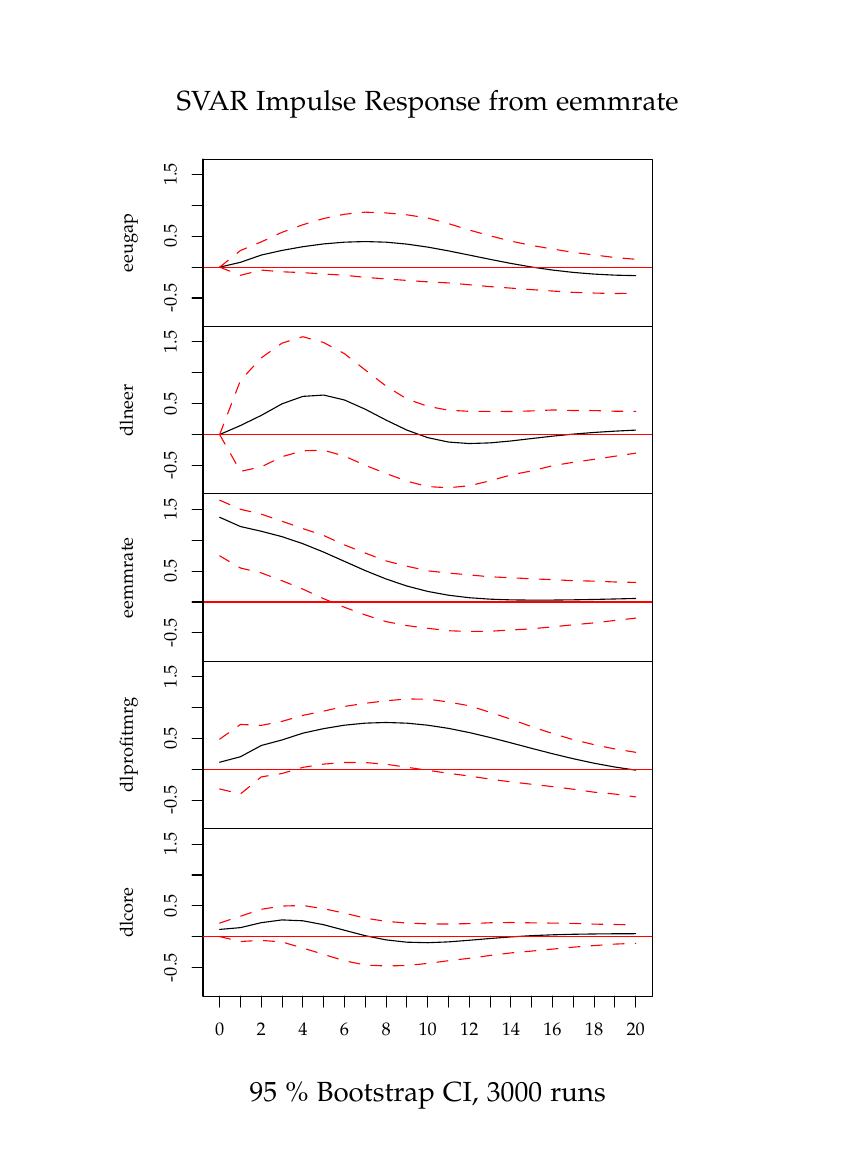
\begin{tikzpicture}[x=1pt,y=1pt]
\definecolor{fillColor}{RGB}{255,255,255}
\path[use as bounding box,fill=fillColor,fill opacity=0.00] (0,0) rectangle (289.08,397.48);
\begin{scope}
\path[clip] ( 63.36,289.48) rectangle (225.72,349.96);
\definecolor{drawColor}{RGB}{0,0,0}

\path[draw=drawColor,line width= 0.4pt,line join=round,line cap=round] ( 69.37,310.94) --
	( 76.89,312.69) --
	( 84.41,315.31) --
	( 91.92,316.99) --
	( 99.44,318.33) --
	(106.96,319.34) --
	(114.47,319.97) --
	(121.99,320.19) --
	(129.51,319.96) --
	(137.02,319.27) --
	(144.54,318.19) --
	(152.06,316.82) --
	(159.57,315.30) --
	(167.09,313.76) --
	(174.61,312.29) --
	(182.12,310.98) --
	(189.64,309.89) --
	(197.16,309.04) --
	(204.67,308.43) --
	(212.19,308.05) --
	(219.71,307.87);
\end{scope}
\begin{scope}
\path[clip] ( 31.68,289.48) rectangle (257.40,349.96);
\definecolor{drawColor}{RGB}{0,0,0}

\node[text=drawColor,anchor=base,inner sep=0pt, outer sep=0pt, scale=  0.66] at (144.54,259.38) {xy{\$}x};

\node[text=drawColor,rotate= 90.00,anchor=base,inner sep=0pt, outer sep=0pt, scale=  0.66] at ( 38.02,319.72) {eeugap};
\end{scope}
\begin{scope}
\path[clip] (  0.00,  0.00) rectangle (289.08,397.48);
\definecolor{drawColor}{RGB}{0,0,0}

\path[draw=drawColor,line width= 0.4pt,line join=round,line cap=round] ( 63.36,299.78) -- ( 63.36,349.97);

\path[draw=drawColor,line width= 0.4pt,line join=round,line cap=round] ( 63.36,299.78) -- ( 59.40,299.78);

\path[draw=drawColor,line width= 0.4pt,line join=round,line cap=round] ( 63.36,310.94) -- ( 59.40,310.94);

\path[draw=drawColor,line width= 0.4pt,line join=round,line cap=round] ( 63.36,322.10) -- ( 59.40,322.10);

\path[draw=drawColor,line width= 0.4pt,line join=round,line cap=round] ( 63.36,333.26) -- ( 59.40,333.26);

\path[draw=drawColor,line width= 0.4pt,line join=round,line cap=round] ( 63.36,344.42) -- ( 59.40,344.42);

\node[text=drawColor,rotate= 90.00,anchor=base,inner sep=0pt, outer sep=0pt, scale=  0.66] at ( 53.86,299.78) {-0.5};

\node[text=drawColor,rotate= 90.00,anchor=base,inner sep=0pt, outer sep=0pt, scale=  0.66] at ( 53.86,322.10) {0.5};

\node[text=drawColor,rotate= 90.00,anchor=base,inner sep=0pt, outer sep=0pt, scale=  0.66] at ( 53.86,344.42) {1.5};
\end{scope}
\begin{scope}
\path[clip] ( 63.36,289.48) rectangle (225.72,349.96);
\definecolor{drawColor}{RGB}{255,0,0}

\path[draw=drawColor,line width= 0.4pt,line join=round,line cap=round] ( 63.36,310.94) -- (225.72,310.94);

\path[draw=drawColor,line width= 0.4pt,dash pattern=on 4pt off 4pt ,line join=round,line cap=round] ( 69.37,310.94) --
	( 76.89,316.95) --
	( 84.41,320.07) --
	( 91.92,323.54) --
	( 99.44,326.26) --
	(106.96,328.52) --
	(114.47,330.06) --
	(121.99,330.81) --
	(129.51,330.53) --
	(137.02,329.85) --
	(144.54,328.70) --
	(152.06,326.67) --
	(159.57,324.35) --
	(167.09,322.27) --
	(174.61,320.35) --
	(182.12,318.77) --
	(189.64,317.50) --
	(197.16,316.28) --
	(204.67,315.35) --
	(212.19,314.42) --
	(219.71,313.79);

\path[draw=drawColor,line width= 0.4pt,dash pattern=on 4pt off 4pt ,line join=round,line cap=round] ( 69.37,310.94) --
	( 76.89,308.00) --
	( 84.41,309.89) --
	( 91.92,309.26) --
	( 99.44,308.96) --
	(106.96,308.46) --
	(114.47,308.02) --
	(121.99,307.25) --
	(129.51,306.68) --
	(137.02,306.14) --
	(144.54,305.63) --
	(152.06,305.25) --
	(159.57,304.58) --
	(167.09,303.90) --
	(174.61,303.37) --
	(182.12,302.82) --
	(189.64,302.31) --
	(197.16,301.83) --
	(204.67,301.58) --
	(212.19,301.41) --
	(219.71,301.50);
\end{scope}
\begin{scope}
\path[clip] (  0.00,  0.00) rectangle (289.08,397.48);
\definecolor{drawColor}{RGB}{0,0,0}

\path[draw=drawColor,line width= 0.4pt,line join=round,line cap=round] ( 63.36,289.48) --
	(225.72,289.48) --
	(225.72,349.96) --
	( 63.36,349.96) --
	( 63.36,289.48);
\end{scope}
\begin{scope}
\path[clip] ( 63.36,228.99) rectangle (225.72,289.48);
\definecolor{drawColor}{RGB}{0,0,0}

\path[draw=drawColor,line width= 0.4pt,line join=round,line cap=round] ( 69.37,250.45) --
	( 76.89,253.71) --
	( 84.41,257.37) --
	( 91.92,261.56) --
	( 99.44,264.24) --
	(106.96,264.72) --
	(114.47,262.94) --
	(121.99,259.60) --
	(129.51,255.68) --
	(137.02,252.06) --
	(144.54,249.34) --
	(152.06,247.74) --
	(159.57,247.20) --
	(167.09,247.44) --
	(174.61,248.13) --
	(182.12,249.01) --
	(189.64,249.87) --
	(197.16,250.61) --
	(204.67,251.21) --
	(212.19,251.68) --
	(219.71,252.06);
\end{scope}
\begin{scope}
\path[clip] ( 31.68,228.99) rectangle (257.40,289.48);
\definecolor{drawColor}{RGB}{0,0,0}

\node[text=drawColor,anchor=base,inner sep=0pt, outer sep=0pt, scale=  0.66] at (144.54,198.89) {xy{\$}x};

\node[text=drawColor,rotate= 90.00,anchor=base,inner sep=0pt, outer sep=0pt, scale=  0.66] at ( 38.02,259.23) {dlneer};
\end{scope}
\begin{scope}
\path[clip] (  0.00,  0.00) rectangle (289.08,397.48);
\definecolor{drawColor}{RGB}{0,0,0}

\path[draw=drawColor,line width= 0.4pt,line join=round,line cap=round] ( 63.36,239.29) -- ( 63.36,289.48);

\path[draw=drawColor,line width= 0.4pt,line join=round,line cap=round] ( 63.36,239.29) -- ( 59.40,239.29);

\path[draw=drawColor,line width= 0.4pt,line join=round,line cap=round] ( 63.36,250.45) -- ( 59.40,250.45);

\path[draw=drawColor,line width= 0.4pt,line join=round,line cap=round] ( 63.36,261.61) -- ( 59.40,261.61);

\path[draw=drawColor,line width= 0.4pt,line join=round,line cap=round] ( 63.36,272.77) -- ( 59.40,272.77);

\path[draw=drawColor,line width= 0.4pt,line join=round,line cap=round] ( 63.36,283.93) -- ( 59.40,283.93);

\node[text=drawColor,rotate= 90.00,anchor=base,inner sep=0pt, outer sep=0pt, scale=  0.66] at ( 53.86,239.29) {-0.5};

\node[text=drawColor,rotate= 90.00,anchor=base,inner sep=0pt, outer sep=0pt, scale=  0.66] at ( 53.86,261.61) {0.5};

\node[text=drawColor,rotate= 90.00,anchor=base,inner sep=0pt, outer sep=0pt, scale=  0.66] at ( 53.86,283.93) {1.5};
\end{scope}
\begin{scope}
\path[clip] ( 63.36,228.99) rectangle (225.72,289.48);
\definecolor{drawColor}{RGB}{255,0,0}

\path[draw=drawColor,line width= 0.4pt,line join=round,line cap=round] ( 63.36,250.45) -- (225.72,250.45);

\path[draw=drawColor,line width= 0.4pt,dash pattern=on 4pt off 4pt ,line join=round,line cap=round] ( 69.37,250.45) --
	( 76.89,270.02) --
	( 84.41,278.16) --
	( 91.92,283.49) --
	( 99.44,285.80) --
	(106.96,283.69) --
	(114.47,279.68) --
	(121.99,273.77) --
	(129.51,267.96) --
	(137.02,263.30) --
	(144.54,260.67) --
	(152.06,259.24) --
	(159.57,258.85) --
	(167.09,258.84) --
	(174.61,258.78) --
	(182.12,258.99) --
	(189.64,259.34) --
	(197.16,259.14) --
	(204.67,259.12) --
	(212.19,258.88) --
	(219.71,258.81);

\path[draw=drawColor,line width= 0.4pt,dash pattern=on 4pt off 4pt ,line join=round,line cap=round] ( 69.37,250.45) --
	( 76.89,237.15) --
	( 84.41,238.76) --
	( 91.92,242.45) --
	( 99.44,244.59) --
	(106.96,244.78) --
	(114.47,242.66) --
	(121.99,239.34) --
	(129.51,236.38) --
	(137.02,233.61) --
	(144.54,231.65) --
	(152.06,231.23) --
	(159.57,231.95) --
	(167.09,233.73) --
	(174.61,235.87) --
	(182.12,237.32) --
	(189.64,239.19) --
	(197.16,240.43) --
	(204.67,241.50) --
	(212.19,242.62) --
	(219.71,243.72);
\end{scope}
\begin{scope}
\path[clip] (  0.00,  0.00) rectangle (289.08,397.48);
\definecolor{drawColor}{RGB}{0,0,0}

\path[draw=drawColor,line width= 0.4pt,line join=round,line cap=round] ( 63.36,228.99) --
	(225.72,228.99) --
	(225.72,289.48) --
	( 63.36,289.48) --
	( 63.36,228.99);
\end{scope}
\begin{scope}
\path[clip] ( 63.36,168.50) rectangle (225.72,228.99);
\definecolor{drawColor}{RGB}{0,0,0}

\path[draw=drawColor,line width= 0.4pt,line join=round,line cap=round] ( 69.37,220.56) --
	( 76.89,217.21) --
	( 84.41,215.51) --
	( 91.92,213.55) --
	( 99.44,211.01) --
	(106.96,207.97) --
	(114.47,204.63) --
	(121.99,201.29) --
	(129.51,198.26) --
	(137.02,195.72) --
	(144.54,193.77) --
	(152.06,192.39) --
	(159.57,191.49) --
	(167.09,190.97) --
	(174.61,190.71) --
	(182.12,190.62) --
	(189.64,190.64) --
	(197.16,190.73) --
	(204.67,190.87) --
	(212.19,191.04) --
	(219.71,191.22);
\end{scope}
\begin{scope}
\path[clip] ( 31.68,168.50) rectangle (257.40,228.99);
\definecolor{drawColor}{RGB}{0,0,0}

\node[text=drawColor,anchor=base,inner sep=0pt, outer sep=0pt, scale=  0.66] at (144.54,138.40) {xy{\$}x};

\node[text=drawColor,rotate= 90.00,anchor=base,inner sep=0pt, outer sep=0pt, scale=  0.66] at ( 38.02,198.74) {eemmrate};
\end{scope}
\begin{scope}
\path[clip] (  0.00,  0.00) rectangle (289.08,397.48);
\definecolor{drawColor}{RGB}{0,0,0}

\path[draw=drawColor,line width= 0.4pt,line join=round,line cap=round] ( 63.36,178.80) -- ( 63.36,228.99);

\path[draw=drawColor,line width= 0.4pt,line join=round,line cap=round] ( 63.36,178.80) -- ( 59.40,178.80);

\path[draw=drawColor,line width= 0.4pt,line join=round,line cap=round] ( 63.36,189.96) -- ( 59.40,189.96);

\path[draw=drawColor,line width= 0.4pt,line join=round,line cap=round] ( 63.36,201.12) -- ( 59.40,201.12);

\path[draw=drawColor,line width= 0.4pt,line join=round,line cap=round] ( 63.36,212.28) -- ( 59.40,212.28);

\path[draw=drawColor,line width= 0.4pt,line join=round,line cap=round] ( 63.36,223.44) -- ( 59.40,223.44);

\node[text=drawColor,rotate= 90.00,anchor=base,inner sep=0pt, outer sep=0pt, scale=  0.66] at ( 53.86,178.80) {-0.5};

\node[text=drawColor,rotate= 90.00,anchor=base,inner sep=0pt, outer sep=0pt, scale=  0.66] at ( 53.86,201.12) {0.5};

\node[text=drawColor,rotate= 90.00,anchor=base,inner sep=0pt, outer sep=0pt, scale=  0.66] at ( 53.86,223.44) {1.5};
\end{scope}
\begin{scope}
\path[clip] ( 63.36,168.50) rectangle (225.72,228.99);
\definecolor{drawColor}{RGB}{255,0,0}

\path[draw=drawColor,line width= 0.4pt,line join=round,line cap=round] ( 63.36,189.96) -- (225.72,189.96);

\path[draw=drawColor,line width= 0.4pt,dash pattern=on 4pt off 4pt ,line join=round,line cap=round] ( 69.37,226.75) --
	( 76.89,223.44) --
	( 84.41,221.69) --
	( 91.92,219.12) --
	( 99.44,216.48) --
	(106.96,213.98) --
	(114.47,210.56) --
	(121.99,207.62) --
	(129.51,204.78) --
	(137.02,202.89) --
	(144.54,201.20) --
	(152.06,200.41) --
	(159.57,199.74) --
	(167.09,199.05) --
	(174.61,198.71) --
	(182.12,198.33) --
	(189.64,198.02) --
	(197.16,197.65) --
	(204.67,197.48) --
	(212.19,197.18) --
	(219.71,197.02);

\path[draw=drawColor,line width= 0.4pt,dash pattern=on 4pt off 4pt ,line join=round,line cap=round] ( 69.37,206.61) --
	( 76.89,202.23) --
	( 84.41,200.46) --
	( 91.92,197.63) --
	( 99.44,194.60) --
	(106.96,191.13) --
	(114.47,188.04) --
	(121.99,185.27) --
	(129.51,182.85) --
	(137.02,181.42) --
	(144.54,180.45) --
	(152.06,179.56) --
	(159.57,179.29) --
	(167.09,179.38) --
	(174.61,179.82) --
	(182.12,180.25) --
	(189.64,180.97) --
	(197.16,181.71) --
	(204.67,182.40) --
	(212.19,183.28) --
	(219.71,184.12);
\end{scope}
\begin{scope}
\path[clip] (  0.00,  0.00) rectangle (289.08,397.48);
\definecolor{drawColor}{RGB}{0,0,0}

\path[draw=drawColor,line width= 0.4pt,line join=round,line cap=round] ( 63.36,168.50) --
	(225.72,168.50) --
	(225.72,228.99) --
	( 63.36,228.99) --
	( 63.36,168.50);
\end{scope}
\begin{scope}
\path[clip] ( 63.36,108.01) rectangle (225.72,168.50);
\definecolor{drawColor}{RGB}{0,0,0}

\path[draw=drawColor,line width= 0.4pt,line join=round,line cap=round] ( 69.37,132.04) --
	( 76.89,134.03) --
	( 84.41,138.09) --
	( 91.92,140.10) --
	( 99.44,142.55) --
	(106.96,144.19) --
	(114.47,145.43) --
	(121.99,146.17) --
	(129.51,146.41) --
	(137.02,146.16) --
	(144.54,145.43) --
	(152.06,144.28) --
	(159.57,142.77) --
	(167.09,140.99) --
	(174.61,139.05) --
	(182.12,137.06) --
	(189.64,135.12) --
	(197.16,133.31) --
	(204.67,131.69) --
	(212.19,130.31) --
	(219.71,129.19);
\end{scope}
\begin{scope}
\path[clip] ( 31.68,108.01) rectangle (257.40,168.50);
\definecolor{drawColor}{RGB}{0,0,0}

\node[text=drawColor,anchor=base,inner sep=0pt, outer sep=0pt, scale=  0.66] at (144.54, 77.91) {xy{\$}x};

\node[text=drawColor,rotate= 90.00,anchor=base,inner sep=0pt, outer sep=0pt, scale=  0.66] at ( 38.02,138.25) {dlprofitmrg};
\end{scope}
\begin{scope}
\path[clip] (  0.00,  0.00) rectangle (289.08,397.48);
\definecolor{drawColor}{RGB}{0,0,0}

\path[draw=drawColor,line width= 0.4pt,line join=round,line cap=round] ( 63.36,118.31) -- ( 63.36,168.50);

\path[draw=drawColor,line width= 0.4pt,line join=round,line cap=round] ( 63.36,118.31) -- ( 59.40,118.31);

\path[draw=drawColor,line width= 0.4pt,line join=round,line cap=round] ( 63.36,129.47) -- ( 59.40,129.47);

\path[draw=drawColor,line width= 0.4pt,line join=round,line cap=round] ( 63.36,140.63) -- ( 59.40,140.63);

\path[draw=drawColor,line width= 0.4pt,line join=round,line cap=round] ( 63.36,151.79) -- ( 59.40,151.79);

\path[draw=drawColor,line width= 0.4pt,line join=round,line cap=round] ( 63.36,162.95) -- ( 59.40,162.95);

\node[text=drawColor,rotate= 90.00,anchor=base,inner sep=0pt, outer sep=0pt, scale=  0.66] at ( 53.86,118.31) {-0.5};

\node[text=drawColor,rotate= 90.00,anchor=base,inner sep=0pt, outer sep=0pt, scale=  0.66] at ( 53.86,140.63) {0.5};

\node[text=drawColor,rotate= 90.00,anchor=base,inner sep=0pt, outer sep=0pt, scale=  0.66] at ( 53.86,162.95) {1.5};
\end{scope}
\begin{scope}
\path[clip] ( 63.36,108.01) rectangle (225.72,168.50);
\definecolor{drawColor}{RGB}{255,0,0}

\path[draw=drawColor,line width= 0.4pt,line join=round,line cap=round] ( 63.36,129.47) -- (225.72,129.47);

\path[draw=drawColor,line width= 0.4pt,dash pattern=on 4pt off 4pt ,line join=round,line cap=round] ( 69.37,140.39) --
	( 76.89,145.69) --
	( 84.41,145.37) --
	( 91.92,146.82) --
	( 99.44,148.97) --
	(106.96,150.53) --
	(114.47,152.21) --
	(121.99,153.34) --
	(129.51,154.26) --
	(137.02,154.89) --
	(144.54,154.85) --
	(152.06,153.80) --
	(159.57,152.45) --
	(167.09,150.08) --
	(174.61,147.62) --
	(182.12,144.88) --
	(189.64,142.44) --
	(197.16,140.19) --
	(204.67,138.39) --
	(212.19,136.83) --
	(219.71,135.63);

\path[draw=drawColor,line width= 0.4pt,dash pattern=on 4pt off 4pt ,line join=round,line cap=round] ( 69.37,122.39) --
	( 76.89,120.57) --
	( 84.41,126.74) --
	( 91.92,127.98) --
	( 99.44,130.19) --
	(106.96,131.37) --
	(114.47,131.95) --
	(121.99,131.93) --
	(129.51,131.31) --
	(137.02,130.24) --
	(144.54,129.13) --
	(152.06,128.05) --
	(159.57,127.06) --
	(167.09,125.95) --
	(174.61,124.93) --
	(182.12,124.09) --
	(189.64,123.23) --
	(197.16,122.30) --
	(204.67,121.22) --
	(212.19,120.54) --
	(219.71,119.52);
\end{scope}
\begin{scope}
\path[clip] (  0.00,  0.00) rectangle (289.08,397.48);
\definecolor{drawColor}{RGB}{0,0,0}

\path[draw=drawColor,line width= 0.4pt,line join=round,line cap=round] ( 63.36,108.01) --
	(225.72,108.01) --
	(225.72,168.50) --
	( 63.36,168.50) --
	( 63.36,108.01);
\end{scope}
\begin{scope}
\path[clip] ( 63.36, 47.52) rectangle (225.72,108.01);
\definecolor{drawColor}{RGB}{0,0,0}

\path[draw=drawColor,line width= 0.4pt,line join=round,line cap=round] ( 69.37, 71.63) --
	( 76.89, 72.28) --
	( 84.41, 74.07) --
	( 91.92, 75.07) --
	( 99.44, 74.75) --
	(106.96, 73.33) --
	(114.47, 71.33) --
	(121.99, 69.36) --
	(129.51, 67.85) --
	(137.02, 67.02) --
	(144.54, 66.83) --
	(152.06, 67.13) --
	(159.57, 67.71) --
	(167.09, 68.35) --
	(174.61, 68.93) --
	(182.12, 69.38) --
	(189.64, 69.68) --
	(197.16, 69.88) --
	(204.67, 69.99) --
	(212.19, 70.06) --
	(219.71, 70.09);
\end{scope}
\begin{scope}
\path[clip] ( 31.68, 47.52) rectangle (257.40,108.01);
\definecolor{drawColor}{RGB}{0,0,0}

\node[text=drawColor,anchor=base,inner sep=0pt, outer sep=0pt, scale=  0.66] at (144.54, 17.42) {xy{\$}x};

\node[text=drawColor,rotate= 90.00,anchor=base,inner sep=0pt, outer sep=0pt, scale=  0.66] at ( 38.02, 77.76) {dlcore};
\end{scope}
\begin{scope}
\path[clip] (  0.00,  0.00) rectangle (289.08,397.48);
\definecolor{drawColor}{RGB}{0,0,0}

\path[draw=drawColor,line width= 0.4pt,line join=round,line cap=round] ( 63.36, 57.82) -- ( 63.36,108.01);

\path[draw=drawColor,line width= 0.4pt,line join=round,line cap=round] ( 63.36, 57.82) -- ( 59.40, 57.82);

\path[draw=drawColor,line width= 0.4pt,line join=round,line cap=round] ( 63.36, 68.98) -- ( 59.40, 68.98);

\path[draw=drawColor,line width= 0.4pt,line join=round,line cap=round] ( 63.36, 80.14) -- ( 59.40, 80.14);

\path[draw=drawColor,line width= 0.4pt,line join=round,line cap=round] ( 63.36, 91.30) -- ( 59.40, 91.30);

\path[draw=drawColor,line width= 0.4pt,line join=round,line cap=round] ( 63.36,102.46) -- ( 59.40,102.46);

\node[text=drawColor,rotate= 90.00,anchor=base,inner sep=0pt, outer sep=0pt, scale=  0.66] at ( 53.86, 57.82) {-0.5};

\node[text=drawColor,rotate= 90.00,anchor=base,inner sep=0pt, outer sep=0pt, scale=  0.66] at ( 53.86, 80.14) {0.5};

\node[text=drawColor,rotate= 90.00,anchor=base,inner sep=0pt, outer sep=0pt, scale=  0.66] at ( 53.86,102.46) {1.5};

\path[draw=drawColor,line width= 0.4pt,line join=round,line cap=round] ( 69.37, 47.52) -- (219.71, 47.52);

\path[draw=drawColor,line width= 0.4pt,line join=round,line cap=round] ( 69.37, 47.52) -- ( 69.37, 43.56);

\path[draw=drawColor,line width= 0.4pt,line join=round,line cap=round] ( 76.89, 47.52) -- ( 76.89, 43.56);

\path[draw=drawColor,line width= 0.4pt,line join=round,line cap=round] ( 84.41, 47.52) -- ( 84.41, 43.56);

\path[draw=drawColor,line width= 0.4pt,line join=round,line cap=round] ( 91.92, 47.52) -- ( 91.92, 43.56);

\path[draw=drawColor,line width= 0.4pt,line join=round,line cap=round] ( 99.44, 47.52) -- ( 99.44, 43.56);

\path[draw=drawColor,line width= 0.4pt,line join=round,line cap=round] (106.96, 47.52) -- (106.96, 43.56);

\path[draw=drawColor,line width= 0.4pt,line join=round,line cap=round] (114.47, 47.52) -- (114.47, 43.56);

\path[draw=drawColor,line width= 0.4pt,line join=round,line cap=round] (121.99, 47.52) -- (121.99, 43.56);

\path[draw=drawColor,line width= 0.4pt,line join=round,line cap=round] (129.51, 47.52) -- (129.51, 43.56);

\path[draw=drawColor,line width= 0.4pt,line join=round,line cap=round] (137.02, 47.52) -- (137.02, 43.56);

\path[draw=drawColor,line width= 0.4pt,line join=round,line cap=round] (144.54, 47.52) -- (144.54, 43.56);

\path[draw=drawColor,line width= 0.4pt,line join=round,line cap=round] (152.06, 47.52) -- (152.06, 43.56);

\path[draw=drawColor,line width= 0.4pt,line join=round,line cap=round] (159.57, 47.52) -- (159.57, 43.56);

\path[draw=drawColor,line width= 0.4pt,line join=round,line cap=round] (167.09, 47.52) -- (167.09, 43.56);

\path[draw=drawColor,line width= 0.4pt,line join=round,line cap=round] (174.61, 47.52) -- (174.61, 43.56);

\path[draw=drawColor,line width= 0.4pt,line join=round,line cap=round] (182.12, 47.52) -- (182.12, 43.56);

\path[draw=drawColor,line width= 0.4pt,line join=round,line cap=round] (189.64, 47.52) -- (189.64, 43.56);

\path[draw=drawColor,line width= 0.4pt,line join=round,line cap=round] (197.16, 47.52) -- (197.16, 43.56);

\path[draw=drawColor,line width= 0.4pt,line join=round,line cap=round] (204.67, 47.52) -- (204.67, 43.56);

\path[draw=drawColor,line width= 0.4pt,line join=round,line cap=round] (212.19, 47.52) -- (212.19, 43.56);

\path[draw=drawColor,line width= 0.4pt,line join=round,line cap=round] (219.71, 47.52) -- (219.71, 43.56);

\node[text=drawColor,anchor=base,inner sep=0pt, outer sep=0pt, scale=  0.66] at ( 69.37, 33.26) {0};

\node[text=drawColor,anchor=base,inner sep=0pt, outer sep=0pt, scale=  0.66] at ( 84.41, 33.26) {2};

\node[text=drawColor,anchor=base,inner sep=0pt, outer sep=0pt, scale=  0.66] at ( 99.44, 33.26) {4};

\node[text=drawColor,anchor=base,inner sep=0pt, outer sep=0pt, scale=  0.66] at (114.47, 33.26) {6};

\node[text=drawColor,anchor=base,inner sep=0pt, outer sep=0pt, scale=  0.66] at (129.51, 33.26) {8};

\node[text=drawColor,anchor=base,inner sep=0pt, outer sep=0pt, scale=  0.66] at (144.54, 33.26) {10};

\node[text=drawColor,anchor=base,inner sep=0pt, outer sep=0pt, scale=  0.66] at (159.57, 33.26) {12};

\node[text=drawColor,anchor=base,inner sep=0pt, outer sep=0pt, scale=  0.66] at (174.61, 33.26) {14};

\node[text=drawColor,anchor=base,inner sep=0pt, outer sep=0pt, scale=  0.66] at (189.64, 33.26) {16};

\node[text=drawColor,anchor=base,inner sep=0pt, outer sep=0pt, scale=  0.66] at (204.67, 33.26) {18};

\node[text=drawColor,anchor=base,inner sep=0pt, outer sep=0pt, scale=  0.66] at (219.71, 33.26) {20};

\path[draw=drawColor,line width= 0.4pt,line join=round,line cap=round] ( 63.36, 47.52) --
	(225.72, 47.52) --
	(225.72,108.01) --
	( 63.36,108.01) --
	( 63.36, 47.52);
\end{scope}
\begin{scope}
\path[clip] ( 63.36, 47.52) rectangle (225.72,108.01);
\definecolor{drawColor}{RGB}{255,0,0}

\path[draw=drawColor,line width= 0.4pt,line join=round,line cap=round] ( 63.36, 68.98) -- (225.72, 68.98);

\path[draw=drawColor,line width= 0.4pt,dash pattern=on 4pt off 4pt ,line join=round,line cap=round] ( 69.37, 73.92) --
	( 76.89, 76.41) --
	( 84.41, 78.92) --
	( 91.92, 80.07) --
	( 99.44, 80.29) --
	(106.96, 79.11) --
	(114.47, 77.52) --
	(121.99, 75.69) --
	(129.51, 74.55) --
	(137.02, 73.94) --
	(144.54, 73.63) --
	(152.06, 73.59) --
	(159.57, 73.72) --
	(167.09, 74.03) --
	(174.61, 74.13) --
	(182.12, 74.01) --
	(189.64, 73.92) --
	(197.16, 73.81) --
	(204.67, 73.55) --
	(212.19, 73.41) --
	(219.71, 73.25);

\path[draw=drawColor,line width= 0.4pt,dash pattern=on 4pt off 4pt ,line join=round,line cap=round] ( 69.37, 69.05) --
	( 76.89, 67.27) --
	( 84.41, 67.68) --
	( 91.92, 67.09) --
	( 99.44, 64.90) --
	(106.96, 62.60) --
	(114.47, 60.31) --
	(121.99, 58.77) --
	(129.51, 58.42) --
	(137.02, 58.60) --
	(144.54, 59.34) --
	(152.06, 60.33) --
	(159.57, 61.20) --
	(167.09, 62.23) --
	(174.61, 63.14) --
	(182.12, 63.81) --
	(189.64, 64.52) --
	(197.16, 65.22) --
	(204.67, 65.79) --
	(212.19, 66.33) --
	(219.71, 66.61);
\end{scope}
\begin{scope}
\path[clip] (  0.00,  0.00) rectangle (289.08,397.48);
\definecolor{drawColor}{RGB}{0,0,0}

\node[text=drawColor,anchor=base,inner sep=0pt, outer sep=0pt, scale=  1.00] at (144.54,367.39) {SVAR Impulse Response from eemmrate};

\node[text=drawColor,anchor=base,inner sep=0pt, outer sep=0pt, scale=  1.00] at (144.54,  9.50) {95 {\%} Bootstrap CI,  3000 runs};
\end{scope}
\end{tikzpicture}
}
\vspace*{-10mm}
\caption{Impulse response to unemployment gap shock in VAR}\label{fig:IRS_eemmrate}
% \vspace*{-4mm} %get rid of the nas
% \caption*{Source: EUROSTAT  (namq\_10\_gdp, namq\_10\_lp\_ulc)}
\end{figure}

\begin{figure}[H]
% \centering
\resizebox{12 cm}{!}{% Created by tikzDevice version 0.9 on 2016-01-13 23:40:07
% !TEX encoding = UTF-8 Unicode
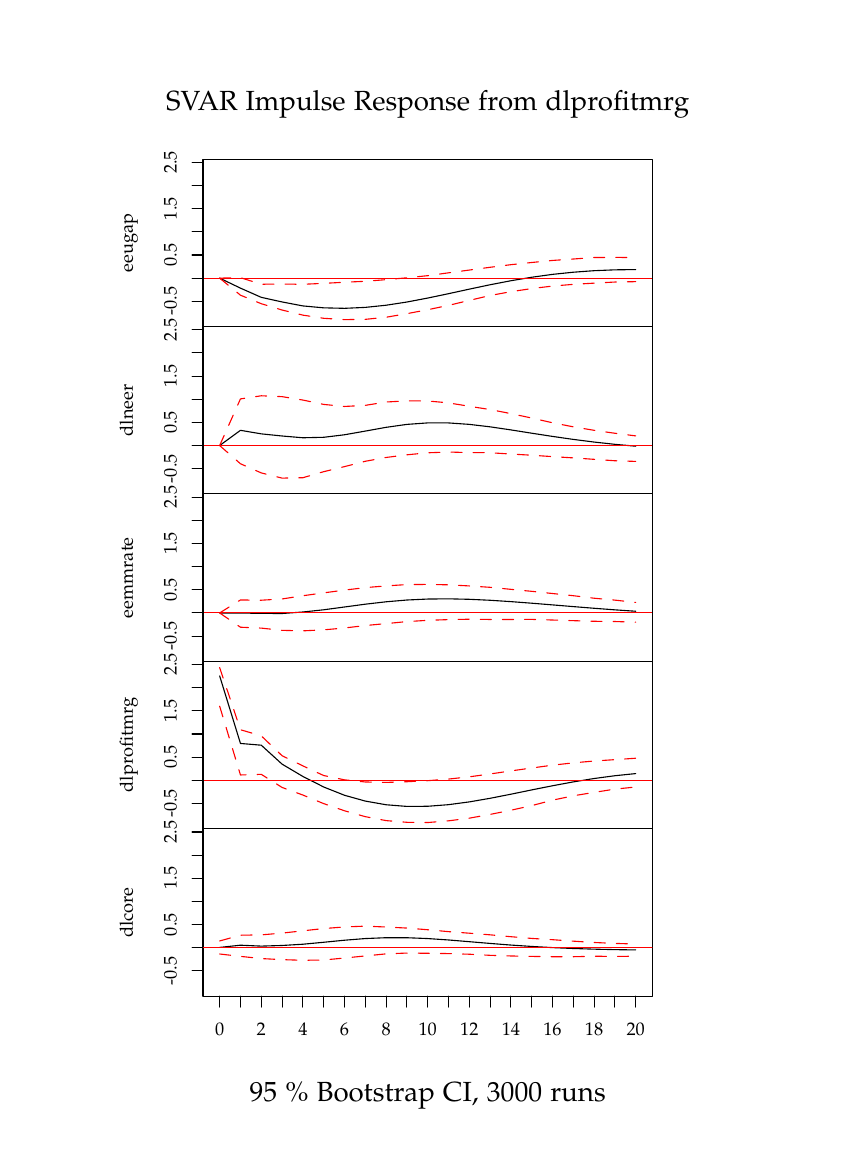
\begin{tikzpicture}[x=1pt,y=1pt]
\definecolor{fillColor}{RGB}{255,255,255}
\path[use as bounding box,fill=fillColor,fill opacity=0.00] (0,0) rectangle (289.08,397.48);
\begin{scope}
\path[clip] ( 63.36,289.48) rectangle (225.72,349.96);
\definecolor{drawColor}{RGB}{0,0,0}

\path[draw=drawColor,line width= 0.4pt,line join=round,line cap=round] ( 69.37,306.97) --
	( 76.89,303.36) --
	( 84.41,300.03) --
	( 91.92,298.37) --
	( 99.44,296.93) --
	(106.96,296.24) --
	(114.47,296.06) --
	(121.99,296.40) --
	(129.51,297.18) --
	(137.02,298.34) --
	(144.54,299.77) --
	(152.06,301.35) --
	(159.57,302.99) --
	(167.09,304.58) --
	(174.61,306.03) --
	(182.12,307.29) --
	(189.64,308.33) --
	(197.16,309.11) --
	(204.67,309.66) --
	(212.19,309.97) --
	(219.71,310.07);
\end{scope}
\begin{scope}
\path[clip] ( 31.68,289.48) rectangle (257.40,349.96);
\definecolor{drawColor}{RGB}{0,0,0}

\node[text=drawColor,anchor=base,inner sep=0pt, outer sep=0pt, scale=  0.66] at (144.54,259.38) {xy{\$}x};

\node[text=drawColor,rotate= 90.00,anchor=base,inner sep=0pt, outer sep=0pt, scale=  0.66] at ( 38.02,319.72) {eeugap};
\end{scope}
\begin{scope}
\path[clip] (  0.00,  0.00) rectangle (289.08,397.48);
\definecolor{drawColor}{RGB}{0,0,0}

\path[draw=drawColor,line width= 0.4pt,line join=round,line cap=round] ( 63.36,298.60) -- ( 63.36,348.81);

\path[draw=drawColor,line width= 0.4pt,line join=round,line cap=round] ( 63.36,298.60) -- ( 59.40,298.60);

\path[draw=drawColor,line width= 0.4pt,line join=round,line cap=round] ( 63.36,306.97) -- ( 59.40,306.97);

\path[draw=drawColor,line width= 0.4pt,line join=round,line cap=round] ( 63.36,315.34) -- ( 59.40,315.34);

\path[draw=drawColor,line width= 0.4pt,line join=round,line cap=round] ( 63.36,323.70) -- ( 59.40,323.70);

\path[draw=drawColor,line width= 0.4pt,line join=round,line cap=round] ( 63.36,332.07) -- ( 59.40,332.07);

\path[draw=drawColor,line width= 0.4pt,line join=round,line cap=round] ( 63.36,340.44) -- ( 59.40,340.44);

\path[draw=drawColor,line width= 0.4pt,line join=round,line cap=round] ( 63.36,348.81) -- ( 59.40,348.81);

\node[text=drawColor,rotate= 90.00,anchor=base,inner sep=0pt, outer sep=0pt, scale=  0.66] at ( 53.86,298.60) {-0.5};

\node[text=drawColor,rotate= 90.00,anchor=base,inner sep=0pt, outer sep=0pt, scale=  0.66] at ( 53.86,315.34) {0.5};

\node[text=drawColor,rotate= 90.00,anchor=base,inner sep=0pt, outer sep=0pt, scale=  0.66] at ( 53.86,332.07) {1.5};

\node[text=drawColor,rotate= 90.00,anchor=base,inner sep=0pt, outer sep=0pt, scale=  0.66] at ( 53.86,348.81) {2.5};
\end{scope}
\begin{scope}
\path[clip] ( 63.36,289.48) rectangle (225.72,349.96);
\definecolor{drawColor}{RGB}{255,0,0}

\path[draw=drawColor,line width= 0.4pt,line join=round,line cap=round] ( 63.36,306.97) -- (225.72,306.97);

\path[draw=drawColor,line width= 0.4pt,dash pattern=on 4pt off 4pt ,line join=round,line cap=round] ( 69.37,306.97) --
	( 76.89,307.14) --
	( 84.41,304.77) --
	( 91.92,304.83) --
	( 99.44,304.75) --
	(106.96,305.08) --
	(114.47,305.49) --
	(121.99,305.83) --
	(129.51,306.42) --
	(137.02,307.09) --
	(144.54,307.86) --
	(152.06,308.89) --
	(159.57,309.89) --
	(167.09,310.89) --
	(174.61,311.83) --
	(182.12,312.62) --
	(189.64,313.36) --
	(197.16,313.88) --
	(204.67,314.43) --
	(212.19,314.46) --
	(219.71,314.42);

\path[draw=drawColor,line width= 0.4pt,dash pattern=on 4pt off 4pt ,line join=round,line cap=round] ( 69.37,306.97) --
	( 76.89,300.81) --
	( 84.41,297.73) --
	( 91.92,295.45) --
	( 99.44,293.60) --
	(106.96,292.46) --
	(114.47,291.98) --
	(121.99,292.08) --
	(129.51,292.84) --
	(137.02,294.13) --
	(144.54,295.56) --
	(152.06,297.12) --
	(159.57,298.93) --
	(167.09,300.69) --
	(174.61,302.08) --
	(182.12,303.19) --
	(189.64,304.11) --
	(197.16,304.72) --
	(204.67,305.16) --
	(212.19,305.56) --
	(219.71,305.70);
\end{scope}
\begin{scope}
\path[clip] (  0.00,  0.00) rectangle (289.08,397.48);
\definecolor{drawColor}{RGB}{0,0,0}

\path[draw=drawColor,line width= 0.4pt,line join=round,line cap=round] ( 63.36,289.48) --
	(225.72,289.48) --
	(225.72,349.96) --
	( 63.36,349.96) --
	( 63.36,289.48);
\end{scope}
\begin{scope}
\path[clip] ( 63.36,228.99) rectangle (225.72,289.48);
\definecolor{drawColor}{RGB}{0,0,0}

\path[draw=drawColor,line width= 0.4pt,line join=round,line cap=round] ( 69.37,246.48) --
	( 76.89,251.98) --
	( 84.41,250.70) --
	( 91.92,249.93) --
	( 99.44,249.29) --
	(106.96,249.46) --
	(114.47,250.37) --
	(121.99,251.70) --
	(129.51,253.06) --
	(137.02,254.12) --
	(144.54,254.66) --
	(152.06,254.65) --
	(159.57,254.13) --
	(167.09,253.24) --
	(174.61,252.13) --
	(182.12,250.94) --
	(189.64,249.78) --
	(197.16,248.70) --
	(204.67,247.74) --
	(212.19,246.92) --
	(219.71,246.24);
\end{scope}
\begin{scope}
\path[clip] ( 31.68,228.99) rectangle (257.40,289.48);
\definecolor{drawColor}{RGB}{0,0,0}

\node[text=drawColor,anchor=base,inner sep=0pt, outer sep=0pt, scale=  0.66] at (144.54,198.89) {xy{\$}x};

\node[text=drawColor,rotate= 90.00,anchor=base,inner sep=0pt, outer sep=0pt, scale=  0.66] at ( 38.02,259.23) {dlneer};
\end{scope}
\begin{scope}
\path[clip] (  0.00,  0.00) rectangle (289.08,397.48);
\definecolor{drawColor}{RGB}{0,0,0}

\path[draw=drawColor,line width= 0.4pt,line join=round,line cap=round] ( 63.36,238.11) -- ( 63.36,288.32);

\path[draw=drawColor,line width= 0.4pt,line join=round,line cap=round] ( 63.36,238.11) -- ( 59.40,238.11);

\path[draw=drawColor,line width= 0.4pt,line join=round,line cap=round] ( 63.36,246.48) -- ( 59.40,246.48);

\path[draw=drawColor,line width= 0.4pt,line join=round,line cap=round] ( 63.36,254.85) -- ( 59.40,254.85);

\path[draw=drawColor,line width= 0.4pt,line join=round,line cap=round] ( 63.36,263.21) -- ( 59.40,263.21);

\path[draw=drawColor,line width= 0.4pt,line join=round,line cap=round] ( 63.36,271.58) -- ( 59.40,271.58);

\path[draw=drawColor,line width= 0.4pt,line join=round,line cap=round] ( 63.36,279.95) -- ( 59.40,279.95);

\path[draw=drawColor,line width= 0.4pt,line join=round,line cap=round] ( 63.36,288.32) -- ( 59.40,288.32);

\node[text=drawColor,rotate= 90.00,anchor=base,inner sep=0pt, outer sep=0pt, scale=  0.66] at ( 53.86,238.11) {-0.5};

\node[text=drawColor,rotate= 90.00,anchor=base,inner sep=0pt, outer sep=0pt, scale=  0.66] at ( 53.86,254.85) {0.5};

\node[text=drawColor,rotate= 90.00,anchor=base,inner sep=0pt, outer sep=0pt, scale=  0.66] at ( 53.86,271.58) {1.5};

\node[text=drawColor,rotate= 90.00,anchor=base,inner sep=0pt, outer sep=0pt, scale=  0.66] at ( 53.86,288.32) {2.5};
\end{scope}
\begin{scope}
\path[clip] ( 63.36,228.99) rectangle (225.72,289.48);
\definecolor{drawColor}{RGB}{255,0,0}

\path[draw=drawColor,line width= 0.4pt,line join=round,line cap=round] ( 63.36,246.48) -- (225.72,246.48);

\path[draw=drawColor,line width= 0.4pt,dash pattern=on 4pt off 4pt ,line join=round,line cap=round] ( 69.37,246.48) --
	( 76.89,263.33) --
	( 84.41,264.46) --
	( 91.92,264.15) --
	( 99.44,262.92) --
	(106.96,261.34) --
	(114.47,260.60) --
	(121.99,261.00) --
	(129.51,262.21) --
	(137.02,262.62) --
	(144.54,262.58) --
	(152.06,261.90) --
	(159.57,260.66) --
	(167.09,259.49) --
	(174.61,258.02) --
	(182.12,256.42) --
	(189.64,254.71) --
	(197.16,253.24) --
	(204.67,251.98) --
	(212.19,250.92) --
	(219.71,249.97);

\path[draw=drawColor,line width= 0.4pt,dash pattern=on 4pt off 4pt ,line join=round,line cap=round] ( 69.37,246.48) --
	( 76.89,239.90) --
	( 84.41,236.59) --
	( 91.92,234.71) --
	( 99.44,234.85) --
	(106.96,237.03) --
	(114.47,238.86) --
	(121.99,240.79) --
	(129.51,242.17) --
	(137.02,243.13) --
	(144.54,243.86) --
	(152.06,244.13) --
	(159.57,243.94) --
	(167.09,243.88) --
	(174.61,243.41) --
	(182.12,242.98) --
	(189.64,242.48) --
	(197.16,242.02) --
	(204.67,241.50) --
	(212.19,240.98) --
	(219.71,240.75);
\end{scope}
\begin{scope}
\path[clip] (  0.00,  0.00) rectangle (289.08,397.48);
\definecolor{drawColor}{RGB}{0,0,0}

\path[draw=drawColor,line width= 0.4pt,line join=round,line cap=round] ( 63.36,228.99) --
	(225.72,228.99) --
	(225.72,289.48) --
	( 63.36,289.48) --
	( 63.36,228.99);
\end{scope}
\begin{scope}
\path[clip] ( 63.36,168.50) rectangle (225.72,228.99);
\definecolor{drawColor}{RGB}{0,0,0}

\path[draw=drawColor,line width= 0.4pt,line join=round,line cap=round] ( 69.37,185.99) --
	( 76.89,185.96) --
	( 84.41,185.83) --
	( 91.92,185.79) --
	( 99.44,186.33) --
	(106.96,187.13) --
	(114.47,188.14) --
	(121.99,189.15) --
	(129.51,190.02) --
	(137.02,190.66) --
	(144.54,191.01) --
	(152.06,191.09) --
	(159.57,190.92) --
	(167.09,190.57) --
	(174.61,190.08) --
	(182.12,189.51) --
	(189.64,188.90) --
	(197.16,188.28) --
	(204.67,187.68) --
	(212.19,187.11) --
	(219.71,186.60);
\end{scope}
\begin{scope}
\path[clip] ( 31.68,168.50) rectangle (257.40,228.99);
\definecolor{drawColor}{RGB}{0,0,0}

\node[text=drawColor,anchor=base,inner sep=0pt, outer sep=0pt, scale=  0.66] at (144.54,138.40) {xy{\$}x};

\node[text=drawColor,rotate= 90.00,anchor=base,inner sep=0pt, outer sep=0pt, scale=  0.66] at ( 38.02,198.74) {eemmrate};
\end{scope}
\begin{scope}
\path[clip] (  0.00,  0.00) rectangle (289.08,397.48);
\definecolor{drawColor}{RGB}{0,0,0}

\path[draw=drawColor,line width= 0.4pt,line join=round,line cap=round] ( 63.36,177.62) -- ( 63.36,227.83);

\path[draw=drawColor,line width= 0.4pt,line join=round,line cap=round] ( 63.36,177.62) -- ( 59.40,177.62);

\path[draw=drawColor,line width= 0.4pt,line join=round,line cap=round] ( 63.36,185.99) -- ( 59.40,185.99);

\path[draw=drawColor,line width= 0.4pt,line join=round,line cap=round] ( 63.36,194.36) -- ( 59.40,194.36);

\path[draw=drawColor,line width= 0.4pt,line join=round,line cap=round] ( 63.36,202.73) -- ( 59.40,202.73);

\path[draw=drawColor,line width= 0.4pt,line join=round,line cap=round] ( 63.36,211.09) -- ( 59.40,211.09);

\path[draw=drawColor,line width= 0.4pt,line join=round,line cap=round] ( 63.36,219.46) -- ( 59.40,219.46);

\path[draw=drawColor,line width= 0.4pt,line join=round,line cap=round] ( 63.36,227.83) -- ( 59.40,227.83);

\node[text=drawColor,rotate= 90.00,anchor=base,inner sep=0pt, outer sep=0pt, scale=  0.66] at ( 53.86,177.62) {-0.5};

\node[text=drawColor,rotate= 90.00,anchor=base,inner sep=0pt, outer sep=0pt, scale=  0.66] at ( 53.86,194.36) {0.5};

\node[text=drawColor,rotate= 90.00,anchor=base,inner sep=0pt, outer sep=0pt, scale=  0.66] at ( 53.86,211.09) {1.5};

\node[text=drawColor,rotate= 90.00,anchor=base,inner sep=0pt, outer sep=0pt, scale=  0.66] at ( 53.86,227.83) {2.5};
\end{scope}
\begin{scope}
\path[clip] ( 63.36,168.50) rectangle (225.72,228.99);
\definecolor{drawColor}{RGB}{255,0,0}

\path[draw=drawColor,line width= 0.4pt,line join=round,line cap=round] ( 63.36,185.99) -- (225.72,185.99);

\path[draw=drawColor,line width= 0.4pt,dash pattern=on 4pt off 4pt ,line join=round,line cap=round] ( 69.37,185.99) --
	( 76.89,190.68) --
	( 84.41,190.59) --
	( 91.92,191.04) --
	( 99.44,192.21) --
	(106.96,193.24) --
	(114.47,194.24) --
	(121.99,195.14) --
	(129.51,195.76) --
	(137.02,196.24) --
	(144.54,196.30) --
	(152.06,196.15) --
	(159.57,195.75) --
	(167.09,195.25) --
	(174.61,194.52) --
	(182.12,193.80) --
	(189.64,193.01) --
	(197.16,192.22) --
	(204.67,191.31) --
	(212.19,190.62) --
	(219.71,189.80);

\path[draw=drawColor,line width= 0.4pt,dash pattern=on 4pt off 4pt ,line join=round,line cap=round] ( 69.37,185.99) --
	( 76.89,180.83) --
	( 84.41,180.51) --
	( 91.92,179.70) --
	( 99.44,179.52) --
	(106.96,179.88) --
	(114.47,180.55) --
	(121.99,181.44) --
	(129.51,182.14) --
	(137.02,182.86) --
	(144.54,183.32) --
	(152.06,183.58) --
	(159.57,183.72) --
	(167.09,183.63) --
	(174.61,183.62) --
	(182.12,183.66) --
	(189.64,183.43) --
	(197.16,183.20) --
	(204.67,182.98) --
	(212.19,182.89) --
	(219.71,182.65);
\end{scope}
\begin{scope}
\path[clip] (  0.00,  0.00) rectangle (289.08,397.48);
\definecolor{drawColor}{RGB}{0,0,0}

\path[draw=drawColor,line width= 0.4pt,line join=round,line cap=round] ( 63.36,168.50) --
	(225.72,168.50) --
	(225.72,228.99) --
	( 63.36,228.99) --
	( 63.36,168.50);
\end{scope}
\begin{scope}
\path[clip] ( 63.36,108.01) rectangle (225.72,168.50);
\definecolor{drawColor}{RGB}{0,0,0}

\path[draw=drawColor,line width= 0.4pt,line join=round,line cap=round] ( 69.37,163.24) --
	( 76.89,138.83) --
	( 84.41,138.20) --
	( 91.92,131.36) --
	( 99.44,126.91) --
	(106.96,123.10) --
	(114.47,120.11) --
	(121.99,118.01) --
	(129.51,116.68) --
	(137.02,116.08) --
	(144.54,116.13) --
	(152.06,116.71) --
	(159.57,117.71) --
	(167.09,119.01) --
	(174.61,120.49) --
	(182.12,122.04) --
	(189.64,123.54) --
	(197.16,124.94) --
	(204.67,126.16) --
	(212.19,127.17) --
	(219.71,127.94);
\end{scope}
\begin{scope}
\path[clip] ( 31.68,108.01) rectangle (257.40,168.50);
\definecolor{drawColor}{RGB}{0,0,0}

\node[text=drawColor,anchor=base,inner sep=0pt, outer sep=0pt, scale=  0.66] at (144.54, 77.91) {xy{\$}x};

\node[text=drawColor,rotate= 90.00,anchor=base,inner sep=0pt, outer sep=0pt, scale=  0.66] at ( 38.02,138.25) {dlprofitmrg};
\end{scope}
\begin{scope}
\path[clip] (  0.00,  0.00) rectangle (289.08,397.48);
\definecolor{drawColor}{RGB}{0,0,0}

\path[draw=drawColor,line width= 0.4pt,line join=round,line cap=round] ( 63.36,117.13) -- ( 63.36,167.34);

\path[draw=drawColor,line width= 0.4pt,line join=round,line cap=round] ( 63.36,117.13) -- ( 59.40,117.13);

\path[draw=drawColor,line width= 0.4pt,line join=round,line cap=round] ( 63.36,125.50) -- ( 59.40,125.50);

\path[draw=drawColor,line width= 0.4pt,line join=round,line cap=round] ( 63.36,133.87) -- ( 59.40,133.87);

\path[draw=drawColor,line width= 0.4pt,line join=round,line cap=round] ( 63.36,142.24) -- ( 59.40,142.24);

\path[draw=drawColor,line width= 0.4pt,line join=round,line cap=round] ( 63.36,150.60) -- ( 59.40,150.60);

\path[draw=drawColor,line width= 0.4pt,line join=round,line cap=round] ( 63.36,158.97) -- ( 59.40,158.97);

\path[draw=drawColor,line width= 0.4pt,line join=round,line cap=round] ( 63.36,167.34) -- ( 59.40,167.34);

\node[text=drawColor,rotate= 90.00,anchor=base,inner sep=0pt, outer sep=0pt, scale=  0.66] at ( 53.86,117.13) {-0.5};

\node[text=drawColor,rotate= 90.00,anchor=base,inner sep=0pt, outer sep=0pt, scale=  0.66] at ( 53.86,133.87) {0.5};

\node[text=drawColor,rotate= 90.00,anchor=base,inner sep=0pt, outer sep=0pt, scale=  0.66] at ( 53.86,150.60) {1.5};

\node[text=drawColor,rotate= 90.00,anchor=base,inner sep=0pt, outer sep=0pt, scale=  0.66] at ( 53.86,167.34) {2.5};
\end{scope}
\begin{scope}
\path[clip] ( 63.36,108.01) rectangle (225.72,168.50);
\definecolor{drawColor}{RGB}{255,0,0}

\path[draw=drawColor,line width= 0.4pt,line join=round,line cap=round] ( 63.36,125.50) -- (225.72,125.50);

\path[draw=drawColor,line width= 0.4pt,dash pattern=on 4pt off 4pt ,line join=round,line cap=round] ( 69.37,166.26) --
	( 76.89,143.79) --
	( 84.41,141.58) --
	( 91.92,134.40) --
	( 99.44,130.73) --
	(106.96,127.24) --
	(114.47,125.69) --
	(121.99,124.91) --
	(129.51,124.75) --
	(137.02,125.00) --
	(144.54,125.38) --
	(152.06,125.96) --
	(159.57,126.77) --
	(167.09,127.80) --
	(174.61,128.91) --
	(182.12,129.96) --
	(189.64,130.98) --
	(197.16,131.82) --
	(204.67,132.48) --
	(212.19,132.98) --
	(219.71,133.49);

\path[draw=drawColor,line width= 0.4pt,dash pattern=on 4pt off 4pt ,line join=round,line cap=round] ( 69.37,152.30) --
	( 76.89,127.44) --
	( 84.41,127.67) --
	( 91.92,122.94) --
	( 99.44,120.19) --
	(106.96,117.09) --
	(114.47,114.51) --
	(121.99,112.38) --
	(129.51,110.95) --
	(137.02,110.34) --
	(144.54,110.25) --
	(152.06,110.87) --
	(159.57,111.83) --
	(167.09,113.19) --
	(174.61,114.70) --
	(182.12,116.37) --
	(189.64,118.33) --
	(197.16,119.92) --
	(204.67,121.15) --
	(212.19,122.33) --
	(219.71,123.09);
\end{scope}
\begin{scope}
\path[clip] (  0.00,  0.00) rectangle (289.08,397.48);
\definecolor{drawColor}{RGB}{0,0,0}

\path[draw=drawColor,line width= 0.4pt,line join=round,line cap=round] ( 63.36,108.01) --
	(225.72,108.01) --
	(225.72,168.50) --
	( 63.36,168.50) --
	( 63.36,108.01);
\end{scope}
\begin{scope}
\path[clip] ( 63.36, 47.52) rectangle (225.72,108.01);
\definecolor{drawColor}{RGB}{0,0,0}

\path[draw=drawColor,line width= 0.4pt,line join=round,line cap=round] ( 69.37, 65.13) --
	( 76.89, 65.93) --
	( 84.41, 65.60) --
	( 91.92, 65.83) --
	( 99.44, 66.28) --
	(106.96, 66.99) --
	(114.47, 67.73) --
	(121.99, 68.33) --
	(129.51, 68.64) --
	(137.02, 68.63) --
	(144.54, 68.33) --
	(152.06, 67.82) --
	(159.57, 67.20) --
	(167.09, 66.57) --
	(174.61, 65.98) --
	(182.12, 65.48) --
	(189.64, 65.06) --
	(197.16, 64.74) --
	(204.67, 64.50) --
	(212.19, 64.33) --
	(219.71, 64.22);
\end{scope}
\begin{scope}
\path[clip] ( 31.68, 47.52) rectangle (257.40,108.01);
\definecolor{drawColor}{RGB}{0,0,0}

\node[text=drawColor,anchor=base,inner sep=0pt, outer sep=0pt, scale=  0.66] at (144.54, 17.42) {xy{\$}x};

\node[text=drawColor,rotate= 90.00,anchor=base,inner sep=0pt, outer sep=0pt, scale=  0.66] at ( 38.02, 77.76) {dlcore};
\end{scope}
\begin{scope}
\path[clip] (  0.00,  0.00) rectangle (289.08,397.48);
\definecolor{drawColor}{RGB}{0,0,0}

\path[draw=drawColor,line width= 0.4pt,line join=round,line cap=round] ( 63.36, 56.64) -- ( 63.36,106.85);

\path[draw=drawColor,line width= 0.4pt,line join=round,line cap=round] ( 63.36, 56.64) -- ( 59.40, 56.64);

\path[draw=drawColor,line width= 0.4pt,line join=round,line cap=round] ( 63.36, 65.01) -- ( 59.40, 65.01);

\path[draw=drawColor,line width= 0.4pt,line join=round,line cap=round] ( 63.36, 73.38) -- ( 59.40, 73.38);

\path[draw=drawColor,line width= 0.4pt,line join=round,line cap=round] ( 63.36, 81.75) -- ( 59.40, 81.75);

\path[draw=drawColor,line width= 0.4pt,line join=round,line cap=round] ( 63.36, 90.12) -- ( 59.40, 90.12);

\path[draw=drawColor,line width= 0.4pt,line join=round,line cap=round] ( 63.36, 98.48) -- ( 59.40, 98.48);

\path[draw=drawColor,line width= 0.4pt,line join=round,line cap=round] ( 63.36,106.85) -- ( 59.40,106.85);

\node[text=drawColor,rotate= 90.00,anchor=base,inner sep=0pt, outer sep=0pt, scale=  0.66] at ( 53.86, 56.64) {-0.5};

\node[text=drawColor,rotate= 90.00,anchor=base,inner sep=0pt, outer sep=0pt, scale=  0.66] at ( 53.86, 73.38) {0.5};

\node[text=drawColor,rotate= 90.00,anchor=base,inner sep=0pt, outer sep=0pt, scale=  0.66] at ( 53.86, 90.12) {1.5};

\node[text=drawColor,rotate= 90.00,anchor=base,inner sep=0pt, outer sep=0pt, scale=  0.66] at ( 53.86,106.85) {2.5};

\path[draw=drawColor,line width= 0.4pt,line join=round,line cap=round] ( 69.37, 47.52) -- (219.71, 47.52);

\path[draw=drawColor,line width= 0.4pt,line join=round,line cap=round] ( 69.37, 47.52) -- ( 69.37, 43.56);

\path[draw=drawColor,line width= 0.4pt,line join=round,line cap=round] ( 76.89, 47.52) -- ( 76.89, 43.56);

\path[draw=drawColor,line width= 0.4pt,line join=round,line cap=round] ( 84.41, 47.52) -- ( 84.41, 43.56);

\path[draw=drawColor,line width= 0.4pt,line join=round,line cap=round] ( 91.92, 47.52) -- ( 91.92, 43.56);

\path[draw=drawColor,line width= 0.4pt,line join=round,line cap=round] ( 99.44, 47.52) -- ( 99.44, 43.56);

\path[draw=drawColor,line width= 0.4pt,line join=round,line cap=round] (106.96, 47.52) -- (106.96, 43.56);

\path[draw=drawColor,line width= 0.4pt,line join=round,line cap=round] (114.47, 47.52) -- (114.47, 43.56);

\path[draw=drawColor,line width= 0.4pt,line join=round,line cap=round] (121.99, 47.52) -- (121.99, 43.56);

\path[draw=drawColor,line width= 0.4pt,line join=round,line cap=round] (129.51, 47.52) -- (129.51, 43.56);

\path[draw=drawColor,line width= 0.4pt,line join=round,line cap=round] (137.02, 47.52) -- (137.02, 43.56);

\path[draw=drawColor,line width= 0.4pt,line join=round,line cap=round] (144.54, 47.52) -- (144.54, 43.56);

\path[draw=drawColor,line width= 0.4pt,line join=round,line cap=round] (152.06, 47.52) -- (152.06, 43.56);

\path[draw=drawColor,line width= 0.4pt,line join=round,line cap=round] (159.57, 47.52) -- (159.57, 43.56);

\path[draw=drawColor,line width= 0.4pt,line join=round,line cap=round] (167.09, 47.52) -- (167.09, 43.56);

\path[draw=drawColor,line width= 0.4pt,line join=round,line cap=round] (174.61, 47.52) -- (174.61, 43.56);

\path[draw=drawColor,line width= 0.4pt,line join=round,line cap=round] (182.12, 47.52) -- (182.12, 43.56);

\path[draw=drawColor,line width= 0.4pt,line join=round,line cap=round] (189.64, 47.52) -- (189.64, 43.56);

\path[draw=drawColor,line width= 0.4pt,line join=round,line cap=round] (197.16, 47.52) -- (197.16, 43.56);

\path[draw=drawColor,line width= 0.4pt,line join=round,line cap=round] (204.67, 47.52) -- (204.67, 43.56);

\path[draw=drawColor,line width= 0.4pt,line join=round,line cap=round] (212.19, 47.52) -- (212.19, 43.56);

\path[draw=drawColor,line width= 0.4pt,line join=round,line cap=round] (219.71, 47.52) -- (219.71, 43.56);

\node[text=drawColor,anchor=base,inner sep=0pt, outer sep=0pt, scale=  0.66] at ( 69.37, 33.26) {0};

\node[text=drawColor,anchor=base,inner sep=0pt, outer sep=0pt, scale=  0.66] at ( 84.41, 33.26) {2};

\node[text=drawColor,anchor=base,inner sep=0pt, outer sep=0pt, scale=  0.66] at ( 99.44, 33.26) {4};

\node[text=drawColor,anchor=base,inner sep=0pt, outer sep=0pt, scale=  0.66] at (114.47, 33.26) {6};

\node[text=drawColor,anchor=base,inner sep=0pt, outer sep=0pt, scale=  0.66] at (129.51, 33.26) {8};

\node[text=drawColor,anchor=base,inner sep=0pt, outer sep=0pt, scale=  0.66] at (144.54, 33.26) {10};

\node[text=drawColor,anchor=base,inner sep=0pt, outer sep=0pt, scale=  0.66] at (159.57, 33.26) {12};

\node[text=drawColor,anchor=base,inner sep=0pt, outer sep=0pt, scale=  0.66] at (174.61, 33.26) {14};

\node[text=drawColor,anchor=base,inner sep=0pt, outer sep=0pt, scale=  0.66] at (189.64, 33.26) {16};

\node[text=drawColor,anchor=base,inner sep=0pt, outer sep=0pt, scale=  0.66] at (204.67, 33.26) {18};

\node[text=drawColor,anchor=base,inner sep=0pt, outer sep=0pt, scale=  0.66] at (219.71, 33.26) {20};

\path[draw=drawColor,line width= 0.4pt,line join=round,line cap=round] ( 63.36, 47.52) --
	(225.72, 47.52) --
	(225.72,108.01) --
	( 63.36,108.01) --
	( 63.36, 47.52);
\end{scope}
\begin{scope}
\path[clip] ( 63.36, 47.52) rectangle (225.72,108.01);
\definecolor{drawColor}{RGB}{255,0,0}

\path[draw=drawColor,line width= 0.4pt,line join=round,line cap=round] ( 63.36, 65.01) -- (225.72, 65.01);

\path[draw=drawColor,line width= 0.4pt,dash pattern=on 4pt off 4pt ,line join=round,line cap=round] ( 69.37, 67.46) --
	( 76.89, 69.54) --
	( 84.41, 69.66) --
	( 91.92, 70.30) --
	( 99.44, 71.12) --
	(106.96, 71.95) --
	(114.47, 72.52) --
	(121.99, 72.82) --
	(129.51, 72.50) --
	(137.02, 72.12) --
	(144.54, 71.52) --
	(152.06, 70.83) --
	(159.57, 70.27) --
	(167.09, 69.68) --
	(174.61, 69.00) --
	(182.12, 68.38) --
	(189.64, 67.92) --
	(197.16, 67.39) --
	(204.67, 66.91) --
	(212.19, 66.58) --
	(219.71, 66.35);

\path[draw=drawColor,line width= 0.4pt,dash pattern=on 4pt off 4pt ,line join=round,line cap=round] ( 69.37, 62.75) --
	( 76.89, 61.89) --
	( 84.41, 61.10) --
	( 91.92, 60.71) --
	( 99.44, 60.48) --
	(106.96, 60.58) --
	(114.47, 61.30) --
	(121.99, 62.05) --
	(129.51, 62.80) --
	(137.02, 63.09) --
	(144.54, 63.01) --
	(152.06, 62.90) --
	(159.57, 62.67) --
	(167.09, 62.27) --
	(174.61, 62.04) --
	(182.12, 61.88) --
	(189.64, 61.77) --
	(197.16, 61.77) --
	(204.67, 61.93) --
	(212.19, 61.90) --
	(219.71, 61.93);
\end{scope}
\begin{scope}
\path[clip] (  0.00,  0.00) rectangle (289.08,397.48);
\definecolor{drawColor}{RGB}{0,0,0}

\node[text=drawColor,anchor=base,inner sep=0pt, outer sep=0pt, scale=  1.00] at (144.54,367.39) {SVAR Impulse Response from dlprofitmrg};

\node[text=drawColor,anchor=base,inner sep=0pt, outer sep=0pt, scale=  1.00] at (144.54,  9.50) {95 {\%} Bootstrap CI,  3000 runs};
\end{scope}
\end{tikzpicture}
}
\vspace*{-10mm}
\caption{Impulse response to unemployment gap shock in VAR}\label{fig:IRS_dlprofitmrg}
% \vspace*{-4mm} %get rid of the nas
% \caption*{Source: EUROSTAT  (namq\_10\_gdp, namq\_10\_lp\_ulc)}
\end{figure}



\begin{figure}[H]
% \centering
\resizebox{12 cm}{!}{% Created by tikzDevice version 0.9 on 2016-01-13 23:40:08
% !TEX encoding = UTF-8 Unicode
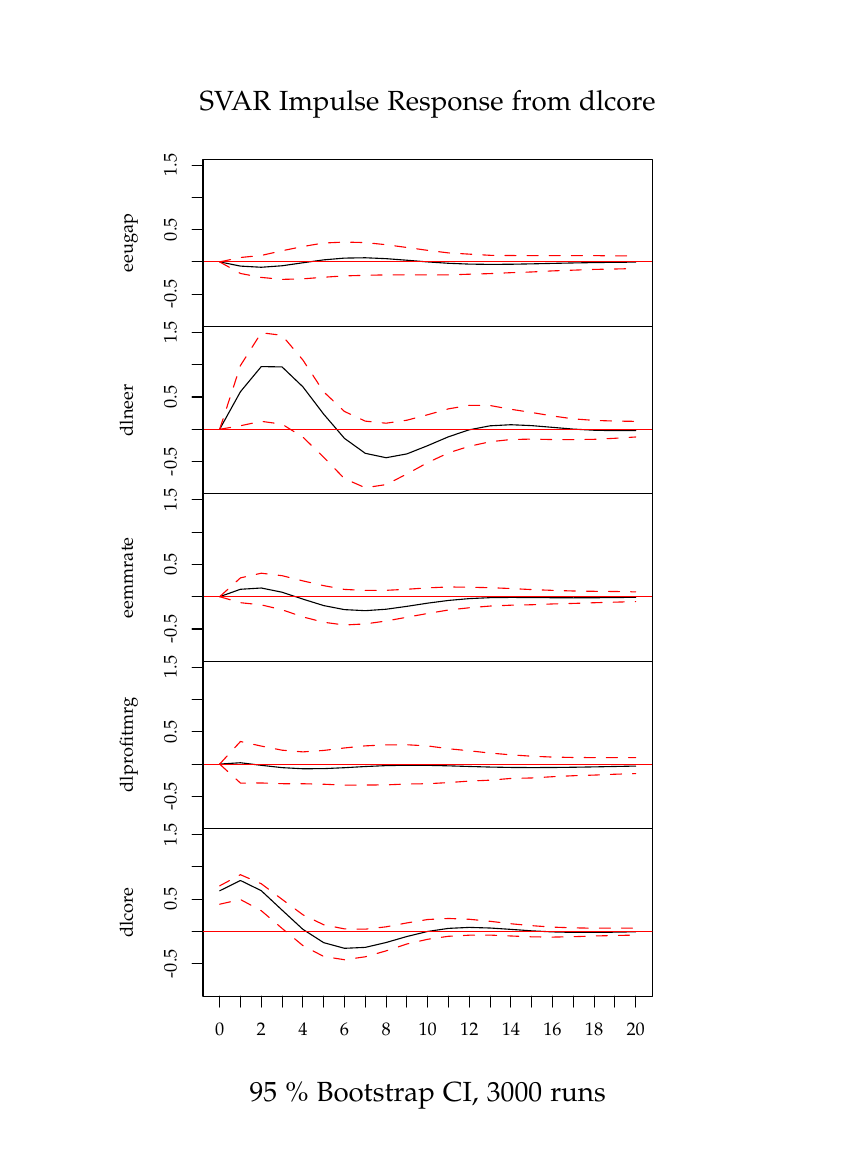
\begin{tikzpicture}[x=1pt,y=1pt]
\definecolor{fillColor}{RGB}{255,255,255}
\path[use as bounding box,fill=fillColor,fill opacity=0.00] (0,0) rectangle (289.08,397.48);
\begin{scope}
\path[clip] ( 63.36,289.48) rectangle (225.72,349.96);
\definecolor{drawColor}{RGB}{0,0,0}

\path[draw=drawColor,line width= 0.4pt,line join=round,line cap=round] ( 69.37,312.84) --
	( 76.89,311.32) --
	( 84.41,310.90) --
	( 91.92,311.44) --
	( 99.44,312.52) --
	(106.96,313.57) --
	(114.47,314.21) --
	(121.99,314.33) --
	(129.51,314.01) --
	(137.02,313.44) --
	(144.54,312.83) --
	(152.06,312.34) --
	(159.57,312.04) --
	(167.09,311.94) --
	(174.61,311.99) --
	(182.12,312.13) --
	(189.64,312.30) --
	(197.16,312.46) --
	(204.67,312.59) --
	(212.19,312.69) --
	(219.71,312.76);
\end{scope}
\begin{scope}
\path[clip] ( 31.68,289.48) rectangle (257.40,349.96);
\definecolor{drawColor}{RGB}{0,0,0}

\node[text=drawColor,anchor=base,inner sep=0pt, outer sep=0pt, scale=  0.66] at (144.54,259.38) {xy{\$}x};

\node[text=drawColor,rotate= 90.00,anchor=base,inner sep=0pt, outer sep=0pt, scale=  0.66] at ( 38.02,319.72) {eeugap};
\end{scope}
\begin{scope}
\path[clip] (  0.00,  0.00) rectangle (289.08,397.48);
\definecolor{drawColor}{RGB}{0,0,0}

\path[draw=drawColor,line width= 0.4pt,line join=round,line cap=round] ( 63.36,301.18) -- ( 63.36,347.82);

\path[draw=drawColor,line width= 0.4pt,line join=round,line cap=round] ( 63.36,301.18) -- ( 59.40,301.18);

\path[draw=drawColor,line width= 0.4pt,line join=round,line cap=round] ( 63.36,312.84) -- ( 59.40,312.84);

\path[draw=drawColor,line width= 0.4pt,line join=round,line cap=round] ( 63.36,324.50) -- ( 59.40,324.50);

\path[draw=drawColor,line width= 0.4pt,line join=round,line cap=round] ( 63.36,336.16) -- ( 59.40,336.16);

\path[draw=drawColor,line width= 0.4pt,line join=round,line cap=round] ( 63.36,347.82) -- ( 59.40,347.82);

\node[text=drawColor,rotate= 90.00,anchor=base,inner sep=0pt, outer sep=0pt, scale=  0.66] at ( 53.86,301.18) {-0.5};

\node[text=drawColor,rotate= 90.00,anchor=base,inner sep=0pt, outer sep=0pt, scale=  0.66] at ( 53.86,324.50) {0.5};

\node[text=drawColor,rotate= 90.00,anchor=base,inner sep=0pt, outer sep=0pt, scale=  0.66] at ( 53.86,347.82) {1.5};
\end{scope}
\begin{scope}
\path[clip] ( 63.36,289.48) rectangle (225.72,349.96);
\definecolor{drawColor}{RGB}{255,0,0}

\path[draw=drawColor,line width= 0.4pt,line join=round,line cap=round] ( 63.36,312.84) -- (225.72,312.84);

\path[draw=drawColor,line width= 0.4pt,dash pattern=on 4pt off 4pt ,line join=round,line cap=round] ( 69.37,312.84) --
	( 76.89,314.43) --
	( 84.41,315.17) --
	( 91.92,316.86) --
	( 99.44,318.40) --
	(106.96,319.66) --
	(114.47,320.00) --
	(121.99,319.82) --
	(129.51,319.05) --
	(137.02,318.05) --
	(144.54,317.01) --
	(152.06,316.09) --
	(159.57,315.64) --
	(167.09,315.22) --
	(174.61,315.14) --
	(182.12,315.09) --
	(189.64,315.10) --
	(197.16,315.13) --
	(204.67,315.11) --
	(212.19,315.01) --
	(219.71,314.98);

\path[draw=drawColor,line width= 0.4pt,dash pattern=on 4pt off 4pt ,line join=round,line cap=round] ( 69.37,312.84) --
	( 76.89,308.65) --
	( 84.41,307.23) --
	( 91.92,306.52) --
	( 99.44,306.71) --
	(106.96,307.30) --
	(114.47,307.78) --
	(121.99,307.99) --
	(129.51,308.15) --
	(137.02,308.14) --
	(144.54,308.14) --
	(152.06,308.14) --
	(159.57,308.39) --
	(167.09,308.61) --
	(174.61,308.94) --
	(182.12,309.20) --
	(189.64,309.59) --
	(197.16,309.85) --
	(204.67,310.12) --
	(212.19,310.27) --
	(219.71,310.44);
\end{scope}
\begin{scope}
\path[clip] (  0.00,  0.00) rectangle (289.08,397.48);
\definecolor{drawColor}{RGB}{0,0,0}

\path[draw=drawColor,line width= 0.4pt,line join=round,line cap=round] ( 63.36,289.48) --
	(225.72,289.48) --
	(225.72,349.96) --
	( 63.36,349.96) --
	( 63.36,289.48);
\end{scope}
\begin{scope}
\path[clip] ( 63.36,228.99) rectangle (225.72,289.48);
\definecolor{drawColor}{RGB}{0,0,0}

\path[draw=drawColor,line width= 0.4pt,line join=round,line cap=round] ( 69.37,252.35) --
	( 76.89,265.94) --
	( 84.41,275.01) --
	( 91.92,274.89) --
	( 99.44,267.71) --
	(106.96,257.82) --
	(114.47,249.07) --
	(121.99,243.67) --
	(129.51,242.08) --
	(137.02,243.46) --
	(144.54,246.44) --
	(152.06,249.65) --
	(159.57,252.17) --
	(167.09,253.61) --
	(174.61,254.00) --
	(182.12,253.68) --
	(189.64,253.05) --
	(197.16,252.42) --
	(204.67,252.01) --
	(212.19,251.85) --
	(219.71,251.91);
\end{scope}
\begin{scope}
\path[clip] ( 31.68,228.99) rectangle (257.40,289.48);
\definecolor{drawColor}{RGB}{0,0,0}

\node[text=drawColor,anchor=base,inner sep=0pt, outer sep=0pt, scale=  0.66] at (144.54,198.89) {xy{\$}x};

\node[text=drawColor,rotate= 90.00,anchor=base,inner sep=0pt, outer sep=0pt, scale=  0.66] at ( 38.02,259.23) {dlneer};
\end{scope}
\begin{scope}
\path[clip] (  0.00,  0.00) rectangle (289.08,397.48);
\definecolor{drawColor}{RGB}{0,0,0}

\path[draw=drawColor,line width= 0.4pt,line join=round,line cap=round] ( 63.36,240.69) -- ( 63.36,287.33);

\path[draw=drawColor,line width= 0.4pt,line join=round,line cap=round] ( 63.36,240.69) -- ( 59.40,240.69);

\path[draw=drawColor,line width= 0.4pt,line join=round,line cap=round] ( 63.36,252.35) -- ( 59.40,252.35);

\path[draw=drawColor,line width= 0.4pt,line join=round,line cap=round] ( 63.36,264.01) -- ( 59.40,264.01);

\path[draw=drawColor,line width= 0.4pt,line join=round,line cap=round] ( 63.36,275.67) -- ( 59.40,275.67);

\path[draw=drawColor,line width= 0.4pt,line join=round,line cap=round] ( 63.36,287.33) -- ( 59.40,287.33);

\node[text=drawColor,rotate= 90.00,anchor=base,inner sep=0pt, outer sep=0pt, scale=  0.66] at ( 53.86,240.69) {-0.5};

\node[text=drawColor,rotate= 90.00,anchor=base,inner sep=0pt, outer sep=0pt, scale=  0.66] at ( 53.86,264.01) {0.5};

\node[text=drawColor,rotate= 90.00,anchor=base,inner sep=0pt, outer sep=0pt, scale=  0.66] at ( 53.86,287.33) {1.5};
\end{scope}
\begin{scope}
\path[clip] ( 63.36,228.99) rectangle (225.72,289.48);
\definecolor{drawColor}{RGB}{255,0,0}

\path[draw=drawColor,line width= 0.4pt,line join=round,line cap=round] ( 63.36,252.35) -- (225.72,252.35);

\path[draw=drawColor,line width= 0.4pt,dash pattern=on 4pt off 4pt ,line join=round,line cap=round] ( 69.37,252.35) --
	( 76.89,275.40) --
	( 84.41,287.24) --
	( 91.92,286.30) --
	( 99.44,277.39) --
	(106.96,265.89) --
	(114.47,258.79) --
	(121.99,255.30) --
	(129.51,254.55) --
	(137.02,255.63) --
	(144.54,257.61) --
	(152.06,259.74) --
	(159.57,261.02) --
	(167.09,260.94) --
	(174.61,259.58) --
	(182.12,258.43) --
	(189.64,257.17) --
	(197.16,256.12) --
	(204.67,255.57) --
	(212.19,255.32) --
	(219.71,255.22);

\path[draw=drawColor,line width= 0.4pt,dash pattern=on 4pt off 4pt ,line join=round,line cap=round] ( 69.37,252.35) --
	( 76.89,253.63) --
	( 84.41,255.23) --
	( 91.92,254.20) --
	( 99.44,249.53) --
	(106.96,242.25) --
	(114.47,234.52) --
	(121.99,231.23) --
	(129.51,232.37) --
	(137.02,236.20) --
	(144.54,240.31) --
	(152.06,243.84) --
	(159.57,246.21) --
	(167.09,247.85) --
	(174.61,248.65) --
	(182.12,248.81) --
	(189.64,248.64) --
	(197.16,248.62) --
	(204.67,248.73) --
	(212.19,249.10) --
	(219.71,249.57);
\end{scope}
\begin{scope}
\path[clip] (  0.00,  0.00) rectangle (289.08,397.48);
\definecolor{drawColor}{RGB}{0,0,0}

\path[draw=drawColor,line width= 0.4pt,line join=round,line cap=round] ( 63.36,228.99) --
	(225.72,228.99) --
	(225.72,289.48) --
	( 63.36,289.48) --
	( 63.36,228.99);
\end{scope}
\begin{scope}
\path[clip] ( 63.36,168.50) rectangle (225.72,228.99);
\definecolor{drawColor}{RGB}{0,0,0}

\path[draw=drawColor,line width= 0.4pt,line join=round,line cap=round] ( 69.37,191.86) --
	( 76.89,194.54) --
	( 84.41,195.00) --
	( 91.92,193.48) --
	( 99.44,190.99) --
	(106.96,188.65) --
	(114.47,187.19) --
	(121.99,186.81) --
	(129.51,187.33) --
	(137.02,188.37) --
	(144.54,189.53) --
	(152.06,190.51) --
	(159.57,191.17) --
	(167.09,191.51) --
	(174.61,191.60) --
	(182.12,191.56) --
	(189.64,191.49) --
	(197.16,191.46) --
	(204.67,191.48) --
	(212.19,191.55) --
	(219.71,191.64);
\end{scope}
\begin{scope}
\path[clip] ( 31.68,168.50) rectangle (257.40,228.99);
\definecolor{drawColor}{RGB}{0,0,0}

\node[text=drawColor,anchor=base,inner sep=0pt, outer sep=0pt, scale=  0.66] at (144.54,138.40) {xy{\$}x};

\node[text=drawColor,rotate= 90.00,anchor=base,inner sep=0pt, outer sep=0pt, scale=  0.66] at ( 38.02,198.74) {eemmrate};
\end{scope}
\begin{scope}
\path[clip] (  0.00,  0.00) rectangle (289.08,397.48);
\definecolor{drawColor}{RGB}{0,0,0}

\path[draw=drawColor,line width= 0.4pt,line join=round,line cap=round] ( 63.36,180.20) -- ( 63.36,226.84);

\path[draw=drawColor,line width= 0.4pt,line join=round,line cap=round] ( 63.36,180.20) -- ( 59.40,180.20);

\path[draw=drawColor,line width= 0.4pt,line join=round,line cap=round] ( 63.36,191.86) -- ( 59.40,191.86);

\path[draw=drawColor,line width= 0.4pt,line join=round,line cap=round] ( 63.36,203.52) -- ( 59.40,203.52);

\path[draw=drawColor,line width= 0.4pt,line join=round,line cap=round] ( 63.36,215.18) -- ( 59.40,215.18);

\path[draw=drawColor,line width= 0.4pt,line join=round,line cap=round] ( 63.36,226.84) -- ( 59.40,226.84);

\node[text=drawColor,rotate= 90.00,anchor=base,inner sep=0pt, outer sep=0pt, scale=  0.66] at ( 53.86,180.20) {-0.5};

\node[text=drawColor,rotate= 90.00,anchor=base,inner sep=0pt, outer sep=0pt, scale=  0.66] at ( 53.86,203.52) {0.5};

\node[text=drawColor,rotate= 90.00,anchor=base,inner sep=0pt, outer sep=0pt, scale=  0.66] at ( 53.86,226.84) {1.5};
\end{scope}
\begin{scope}
\path[clip] ( 63.36,168.50) rectangle (225.72,228.99);
\definecolor{drawColor}{RGB}{255,0,0}

\path[draw=drawColor,line width= 0.4pt,line join=round,line cap=round] ( 63.36,191.86) -- (225.72,191.86);

\path[draw=drawColor,line width= 0.4pt,dash pattern=on 4pt off 4pt ,line join=round,line cap=round] ( 69.37,191.86) --
	( 76.89,198.66) --
	( 84.41,200.35) --
	( 91.92,199.45) --
	( 99.44,197.58) --
	(106.96,195.85) --
	(114.47,194.49) --
	(121.99,194.13) --
	(129.51,194.16) --
	(137.02,194.55) --
	(144.54,195.05) --
	(152.06,195.38) --
	(159.57,195.27) --
	(167.09,195.12) --
	(174.61,194.81) --
	(182.12,194.43) --
	(189.64,194.15) --
	(197.16,193.92) --
	(204.67,193.81) --
	(212.19,193.74) --
	(219.71,193.60);

\path[draw=drawColor,line width= 0.4pt,dash pattern=on 4pt off 4pt ,line join=round,line cap=round] ( 69.37,191.86) --
	( 76.89,189.69) --
	( 84.41,188.91) --
	( 91.92,187.14) --
	( 99.44,184.56) --
	(106.96,182.63) --
	(114.47,181.63) --
	(121.99,182.03) --
	(129.51,183.07) --
	(137.02,184.44) --
	(144.54,185.80) --
	(152.06,187.05) --
	(159.57,187.86) --
	(167.09,188.48) --
	(174.61,188.79) --
	(182.12,188.95) --
	(189.64,189.24) --
	(197.16,189.43) --
	(204.67,189.68) --
	(212.19,189.89) --
	(219.71,190.08);
\end{scope}
\begin{scope}
\path[clip] (  0.00,  0.00) rectangle (289.08,397.48);
\definecolor{drawColor}{RGB}{0,0,0}

\path[draw=drawColor,line width= 0.4pt,line join=round,line cap=round] ( 63.36,168.50) --
	(225.72,168.50) --
	(225.72,228.99) --
	( 63.36,228.99) --
	( 63.36,168.50);
\end{scope}
\begin{scope}
\path[clip] ( 63.36,108.01) rectangle (225.72,168.50);
\definecolor{drawColor}{RGB}{0,0,0}

\path[draw=drawColor,line width= 0.4pt,line join=round,line cap=round] ( 69.37,131.38) --
	( 76.89,131.86) --
	( 84.41,130.93) --
	( 91.92,130.09) --
	( 99.44,129.69) --
	(106.96,129.73) --
	(114.47,130.07) --
	(121.99,130.49) --
	(129.51,130.82) --
	(137.02,130.96) --
	(144.54,130.92) --
	(152.06,130.74) --
	(159.57,130.51) --
	(167.09,130.30) --
	(174.61,130.16) --
	(182.12,130.11) --
	(189.64,130.14) --
	(197.16,130.23) --
	(204.67,130.36) --
	(212.19,130.51) --
	(219.71,130.66);
\end{scope}
\begin{scope}
\path[clip] ( 31.68,108.01) rectangle (257.40,168.50);
\definecolor{drawColor}{RGB}{0,0,0}

\node[text=drawColor,anchor=base,inner sep=0pt, outer sep=0pt, scale=  0.66] at (144.54, 77.91) {xy{\$}x};

\node[text=drawColor,rotate= 90.00,anchor=base,inner sep=0pt, outer sep=0pt, scale=  0.66] at ( 38.02,138.25) {dlprofitmrg};
\end{scope}
\begin{scope}
\path[clip] (  0.00,  0.00) rectangle (289.08,397.48);
\definecolor{drawColor}{RGB}{0,0,0}

\path[draw=drawColor,line width= 0.4pt,line join=round,line cap=round] ( 63.36,119.72) -- ( 63.36,166.36);

\path[draw=drawColor,line width= 0.4pt,line join=round,line cap=round] ( 63.36,119.72) -- ( 59.40,119.72);

\path[draw=drawColor,line width= 0.4pt,line join=round,line cap=round] ( 63.36,131.38) -- ( 59.40,131.38);

\path[draw=drawColor,line width= 0.4pt,line join=round,line cap=round] ( 63.36,143.04) -- ( 59.40,143.04);

\path[draw=drawColor,line width= 0.4pt,line join=round,line cap=round] ( 63.36,154.70) -- ( 59.40,154.70);

\path[draw=drawColor,line width= 0.4pt,line join=round,line cap=round] ( 63.36,166.36) -- ( 59.40,166.36);

\node[text=drawColor,rotate= 90.00,anchor=base,inner sep=0pt, outer sep=0pt, scale=  0.66] at ( 53.86,119.72) {-0.5};

\node[text=drawColor,rotate= 90.00,anchor=base,inner sep=0pt, outer sep=0pt, scale=  0.66] at ( 53.86,143.04) {0.5};

\node[text=drawColor,rotate= 90.00,anchor=base,inner sep=0pt, outer sep=0pt, scale=  0.66] at ( 53.86,166.36) {1.5};
\end{scope}
\begin{scope}
\path[clip] ( 63.36,108.01) rectangle (225.72,168.50);
\definecolor{drawColor}{RGB}{255,0,0}

\path[draw=drawColor,line width= 0.4pt,line join=round,line cap=round] ( 63.36,131.38) -- (225.72,131.38);

\path[draw=drawColor,line width= 0.4pt,dash pattern=on 4pt off 4pt ,line join=round,line cap=round] ( 69.37,131.38) --
	( 76.89,139.54) --
	( 84.41,137.88) --
	( 91.92,136.40) --
	( 99.44,135.78) --
	(106.96,136.31) --
	(114.47,137.20) --
	(121.99,137.96) --
	(129.51,138.32) --
	(137.02,138.36) --
	(144.54,137.94) --
	(152.06,136.92) --
	(159.57,136.18) --
	(167.09,135.36) --
	(174.61,134.72) --
	(182.12,134.22) --
	(189.64,133.91) --
	(197.16,133.76) --
	(204.67,133.72) --
	(212.19,133.72) --
	(219.71,133.73);

\path[draw=drawColor,line width= 0.4pt,dash pattern=on 4pt off 4pt ,line join=round,line cap=round] ( 69.37,131.38) --
	( 76.89,124.51) --
	( 84.41,124.55) --
	( 91.92,124.29) --
	( 99.44,124.27) --
	(106.96,124.10) --
	(114.47,123.75) --
	(121.99,123.81) --
	(129.51,123.86) --
	(137.02,124.18) --
	(144.54,124.28) --
	(152.06,124.69) --
	(159.57,125.23) --
	(167.09,125.56) --
	(174.61,126.19) --
	(182.12,126.36) --
	(189.64,126.81) --
	(197.16,127.17) --
	(204.67,127.40) --
	(212.19,127.71) --
	(219.71,127.93);
\end{scope}
\begin{scope}
\path[clip] (  0.00,  0.00) rectangle (289.08,397.48);
\definecolor{drawColor}{RGB}{0,0,0}

\path[draw=drawColor,line width= 0.4pt,line join=round,line cap=round] ( 63.36,108.01) --
	(225.72,108.01) --
	(225.72,168.50) --
	( 63.36,168.50) --
	( 63.36,108.01);
\end{scope}
\begin{scope}
\path[clip] ( 63.36, 47.52) rectangle (225.72,108.01);
\definecolor{drawColor}{RGB}{0,0,0}

\path[draw=drawColor,line width= 0.4pt,line join=round,line cap=round] ( 69.37, 85.59) --
	( 76.89, 89.31) --
	( 84.41, 85.63) --
	( 91.92, 78.62) --
	( 99.44, 71.67) --
	(106.96, 66.85) --
	(114.47, 64.81) --
	(121.99, 65.14) --
	(129.51, 66.90) --
	(137.02, 69.07) --
	(144.54, 70.90) --
	(152.06, 72.01) --
	(159.57, 72.36) --
	(167.09, 72.14) --
	(174.61, 71.65) --
	(182.12, 71.12) --
	(189.64, 70.74) --
	(197.16, 70.55) --
	(204.67, 70.54) --
	(212.19, 70.64) --
	(219.71, 70.78);
\end{scope}
\begin{scope}
\path[clip] ( 31.68, 47.52) rectangle (257.40,108.01);
\definecolor{drawColor}{RGB}{0,0,0}

\node[text=drawColor,anchor=base,inner sep=0pt, outer sep=0pt, scale=  0.66] at (144.54, 17.42) {xy{\$}x};

\node[text=drawColor,rotate= 90.00,anchor=base,inner sep=0pt, outer sep=0pt, scale=  0.66] at ( 38.02, 77.76) {dlcore};
\end{scope}
\begin{scope}
\path[clip] (  0.00,  0.00) rectangle (289.08,397.48);
\definecolor{drawColor}{RGB}{0,0,0}

\path[draw=drawColor,line width= 0.4pt,line join=round,line cap=round] ( 63.36, 59.23) -- ( 63.36,105.87);

\path[draw=drawColor,line width= 0.4pt,line join=round,line cap=round] ( 63.36, 59.23) -- ( 59.40, 59.23);

\path[draw=drawColor,line width= 0.4pt,line join=round,line cap=round] ( 63.36, 70.89) -- ( 59.40, 70.89);

\path[draw=drawColor,line width= 0.4pt,line join=round,line cap=round] ( 63.36, 82.55) -- ( 59.40, 82.55);

\path[draw=drawColor,line width= 0.4pt,line join=round,line cap=round] ( 63.36, 94.21) -- ( 59.40, 94.21);

\path[draw=drawColor,line width= 0.4pt,line join=round,line cap=round] ( 63.36,105.87) -- ( 59.40,105.87);

\node[text=drawColor,rotate= 90.00,anchor=base,inner sep=0pt, outer sep=0pt, scale=  0.66] at ( 53.86, 59.23) {-0.5};

\node[text=drawColor,rotate= 90.00,anchor=base,inner sep=0pt, outer sep=0pt, scale=  0.66] at ( 53.86, 82.55) {0.5};

\node[text=drawColor,rotate= 90.00,anchor=base,inner sep=0pt, outer sep=0pt, scale=  0.66] at ( 53.86,105.87) {1.5};

\path[draw=drawColor,line width= 0.4pt,line join=round,line cap=round] ( 69.37, 47.52) -- (219.71, 47.52);

\path[draw=drawColor,line width= 0.4pt,line join=round,line cap=round] ( 69.37, 47.52) -- ( 69.37, 43.56);

\path[draw=drawColor,line width= 0.4pt,line join=round,line cap=round] ( 76.89, 47.52) -- ( 76.89, 43.56);

\path[draw=drawColor,line width= 0.4pt,line join=round,line cap=round] ( 84.41, 47.52) -- ( 84.41, 43.56);

\path[draw=drawColor,line width= 0.4pt,line join=round,line cap=round] ( 91.92, 47.52) -- ( 91.92, 43.56);

\path[draw=drawColor,line width= 0.4pt,line join=round,line cap=round] ( 99.44, 47.52) -- ( 99.44, 43.56);

\path[draw=drawColor,line width= 0.4pt,line join=round,line cap=round] (106.96, 47.52) -- (106.96, 43.56);

\path[draw=drawColor,line width= 0.4pt,line join=round,line cap=round] (114.47, 47.52) -- (114.47, 43.56);

\path[draw=drawColor,line width= 0.4pt,line join=round,line cap=round] (121.99, 47.52) -- (121.99, 43.56);

\path[draw=drawColor,line width= 0.4pt,line join=round,line cap=round] (129.51, 47.52) -- (129.51, 43.56);

\path[draw=drawColor,line width= 0.4pt,line join=round,line cap=round] (137.02, 47.52) -- (137.02, 43.56);

\path[draw=drawColor,line width= 0.4pt,line join=round,line cap=round] (144.54, 47.52) -- (144.54, 43.56);

\path[draw=drawColor,line width= 0.4pt,line join=round,line cap=round] (152.06, 47.52) -- (152.06, 43.56);

\path[draw=drawColor,line width= 0.4pt,line join=round,line cap=round] (159.57, 47.52) -- (159.57, 43.56);

\path[draw=drawColor,line width= 0.4pt,line join=round,line cap=round] (167.09, 47.52) -- (167.09, 43.56);

\path[draw=drawColor,line width= 0.4pt,line join=round,line cap=round] (174.61, 47.52) -- (174.61, 43.56);

\path[draw=drawColor,line width= 0.4pt,line join=round,line cap=round] (182.12, 47.52) -- (182.12, 43.56);

\path[draw=drawColor,line width= 0.4pt,line join=round,line cap=round] (189.64, 47.52) -- (189.64, 43.56);

\path[draw=drawColor,line width= 0.4pt,line join=round,line cap=round] (197.16, 47.52) -- (197.16, 43.56);

\path[draw=drawColor,line width= 0.4pt,line join=round,line cap=round] (204.67, 47.52) -- (204.67, 43.56);

\path[draw=drawColor,line width= 0.4pt,line join=round,line cap=round] (212.19, 47.52) -- (212.19, 43.56);

\path[draw=drawColor,line width= 0.4pt,line join=round,line cap=round] (219.71, 47.52) -- (219.71, 43.56);

\node[text=drawColor,anchor=base,inner sep=0pt, outer sep=0pt, scale=  0.66] at ( 69.37, 33.26) {0};

\node[text=drawColor,anchor=base,inner sep=0pt, outer sep=0pt, scale=  0.66] at ( 84.41, 33.26) {2};

\node[text=drawColor,anchor=base,inner sep=0pt, outer sep=0pt, scale=  0.66] at ( 99.44, 33.26) {4};

\node[text=drawColor,anchor=base,inner sep=0pt, outer sep=0pt, scale=  0.66] at (114.47, 33.26) {6};

\node[text=drawColor,anchor=base,inner sep=0pt, outer sep=0pt, scale=  0.66] at (129.51, 33.26) {8};

\node[text=drawColor,anchor=base,inner sep=0pt, outer sep=0pt, scale=  0.66] at (144.54, 33.26) {10};

\node[text=drawColor,anchor=base,inner sep=0pt, outer sep=0pt, scale=  0.66] at (159.57, 33.26) {12};

\node[text=drawColor,anchor=base,inner sep=0pt, outer sep=0pt, scale=  0.66] at (174.61, 33.26) {14};

\node[text=drawColor,anchor=base,inner sep=0pt, outer sep=0pt, scale=  0.66] at (189.64, 33.26) {16};

\node[text=drawColor,anchor=base,inner sep=0pt, outer sep=0pt, scale=  0.66] at (204.67, 33.26) {18};

\node[text=drawColor,anchor=base,inner sep=0pt, outer sep=0pt, scale=  0.66] at (219.71, 33.26) {20};

\path[draw=drawColor,line width= 0.4pt,line join=round,line cap=round] ( 63.36, 47.52) --
	(225.72, 47.52) --
	(225.72,108.01) --
	( 63.36,108.01) --
	( 63.36, 47.52);
\end{scope}
\begin{scope}
\path[clip] ( 63.36, 47.52) rectangle (225.72,108.01);
\definecolor{drawColor}{RGB}{255,0,0}

\path[draw=drawColor,line width= 0.4pt,line join=round,line cap=round] ( 63.36, 70.89) -- (225.72, 70.89);

\path[draw=drawColor,line width= 0.4pt,dash pattern=on 4pt off 4pt ,line join=round,line cap=round] ( 69.37, 87.38) --
	( 76.89, 91.40) --
	( 84.41, 88.14) --
	( 91.92, 82.50) --
	( 99.44, 76.94) --
	(106.96, 73.32) --
	(114.47, 71.83) --
	(121.99, 71.72) --
	(129.51, 72.57) --
	(137.02, 73.98) --
	(144.54, 75.21) --
	(152.06, 75.59) --
	(159.57, 75.30) --
	(167.09, 74.57) --
	(174.61, 73.68) --
	(182.12, 72.99) --
	(189.64, 72.46) --
	(197.16, 72.20) --
	(204.67, 72.07) --
	(212.19, 72.13) --
	(219.71, 72.11);

\path[draw=drawColor,line width= 0.4pt,dash pattern=on 4pt off 4pt ,line join=round,line cap=round] ( 69.37, 80.74) --
	( 76.89, 82.43) --
	( 84.41, 78.40) --
	( 91.92, 72.00) --
	( 99.44, 65.80) --
	(106.96, 61.86) --
	(114.47, 60.68) --
	(121.99, 61.74) --
	(129.51, 63.88) --
	(137.02, 66.37) --
	(144.54, 68.07) --
	(152.06, 69.15) --
	(159.57, 69.55) --
	(167.09, 69.58) --
	(174.61, 69.26) --
	(182.12, 68.95) --
	(189.64, 68.86) --
	(197.16, 69.00) --
	(204.67, 69.26) --
	(212.19, 69.43) --
	(219.71, 69.59);
\end{scope}
\begin{scope}
\path[clip] (  0.00,  0.00) rectangle (289.08,397.48);
\definecolor{drawColor}{RGB}{0,0,0}

\node[text=drawColor,anchor=base,inner sep=0pt, outer sep=0pt, scale=  1.00] at (144.54,367.39) {SVAR Impulse Response from dlcore};

\node[text=drawColor,anchor=base,inner sep=0pt, outer sep=0pt, scale=  1.00] at (144.54,  9.50) {95 {\%} Bootstrap CI,  3000 runs};
\end{scope}
\end{tikzpicture}
}
\vspace*{-10mm}
\caption{Impulse response to unemployment gap shock in VAR}\label{fig:IRS_dlcore}
% \vspace*{-4mm} %get rid of the nas
% \caption*{Source: EUROSTAT  (namq\_10\_gdp, namq\_10\_lp\_ulc)}
\end{figure}
 

\newpage


Again, the core inflation rate moves according to theoretical predictions in a statistically significant manner when we consider that the core inflation rate reacts with a certain time lag. An increase in the nominal exchange rate should reduce the effects of imported inflation and the rebound to the zero level of the nominal exchange rate is followed by a rebound from the negative area to the zero level of the core inflation rate. 


Turing to the short-term interest rate (see Figure \ref{fig:IRS_eemmrate}) which should not have an impact on the structural component of the unemployment gap and in my model the nominal exchange rate (as Estonia has not had an independent monetary policy) it can be seen that a positive shock to the interest rate leads to an immediate response of the profit margin indicator. The profit margin indicator change then increases and becomes slightly signficant after 5 quarters.

 The result is more difficult to explain as most theoretical models and empirical studies do not address the issue how changes in the money market rate should impact the profit margin indicator. In addition, although the money market rate is considered to be endogenous in my model, it is in fact exogenously determined in Frankfurt. 

The response depicted in the last block of Figure \ref{fig:IRS_eemmrate} indicates that a tightening of monetary policy has immediate significant but only slight effect of the core inflation rate in the direction that we would expect. 


Finally, turning to Figure \ref{fig:IRS_dlprofitmrg} it can be seen that when a profit margin shock hits the economy, the core inflation increases by about 0.5\%. The increase is statistically significant. The core inflation rate then returns to the zero growth path. This seems consistent with theoretical predictions and is also in line with the findings of \citet{Neiss2001Markup}. 

%------------------------------------------------


\section{Conclusions}
\label{Conclusions}

This paper provides a primer in the analysis of the Estonian markup and its behaviour over the business cycle. The empirical analysis of the observations of the profit margin indicator as a proxy of the ``true'' markup shows that it moves approximately pro-cyclical over the business cycle. 

The econometric tests point to the evidence for the non-stationarity of the profit margin indicator. Those results are in line with empirical findings for OECD countries \citep{Neiss2001Markup} but contradictory to theoretical models. 

In the next step I construct a SVAR model with standard identifying restrictions. The analysis shows that the movements of the unemployment gap are especially important for understanding the behaviour of the markup. However, the lack of detailed theoretical understanding what causes the unemployment gap to change over time leaves room for interpretation. One possible explanation is that during periods with a higher cyclical unemployment firms have more power to lower wages whereas at the same time keep prices up, resulting in an increase of the markup. This argument is partially supported by the results from Section \ref{Measuring} which show that the gross operating surplus is strongly related to the development of employee compensation. 

Nominal exchange and short-term interest rate shocks cause only small and insignificant responses to the profit margin indicator. Nevertheless, further investigations into open and closed sector markup dynamics and their macroeconomic implications might provide important insights that enhance our understanding of the behaviour of markups. 

Finally, profits margin indicator shocks influence the core inflation rate. This finding has important implications for inflation dynamics. It shows that rising markups contribute positively to the core inflation rate. Thus, further investigations into the possibility of using markups as variables in inflation forecasting models seem to be a fruitful research area.    

  
%----------------------------------------------------------------------------------------
%	REFERENCE LIST
%----------------------------------------------------------------------------------------
\clearpage

\renewcommand*{\bibfont}{\scriptsize}
\printbibliography




\clearpage




% \begin{table}[H]
% \centering
% \begin{tabular}{rrrrr}
%   \hline
%             & Estimate & Std. Error & t value & Pr($>$$|$t$|$) \\
%   \hline
% (Intercept) & 0.012    & 0.007      & 1.740   & 0.086 \\
% z.lag.1     & -0.078   & 0.041      & -1.876  & 0.065 \\
% z.diff.lag1 & -0.110   & 0.119      & -0.923  & 0.359 \\
% z.diff.lag2 & 0.286    & 0.118      & 2.416   & 0.018 \\
% z.diff.lag3 & 0.203    & 0.121      & 1.676   & 0.098 \\
% z.diff.lag4 & 0.033    & 0.117      & 0.282   & 0.779 \\
%    \hline
% \end{tabular}
% \caption{Profit Margin Estonia} 
% \label{PROFITMRG}
% \end{table}
%----------------------------------------------------------------------------------------

\end{multicols}

\end{document}
